\section{Supplementary Information} 
\setcounter{table}{0}
\setcounter{figure}{0}
\pagenumbering{arabic}
\renewcommand*{\thepage}{\arabic{page}}
\renewcommand{\thetable}{S\arabic{table}}
\renewcommand{\thefigure}{S\arabic{figure}}

In the article "Preregistration is important, but not enough", we examine the consequences of two different cases of the data structure; where both the variable of interest $x$ and covariates $z$ have the same distribution i.e., both binary or both normally distributed. However, there are also the cases where one is binary and the other is normally distributed. The result for these cases can be found in this \textit{Supplementary Information} in the section "\nameref{result}". The first figure, \ref{fig:appfigure1}, contains the baseline model. This is the figure that all the other figures are compared to to see the increase of the false-positive probability (FPP) or false-positive ratio (FPR) for any of the flexibilities investigated. For this figure, the sample size is set to 200, the correlation between the dependent variable and covariates is $\textit{r}=0.2$, two covariates are used, and no outlier criteria are used. For each of the figures in this section, one of these flexibilities is changed. Figure \ref{fig:appfigure2} illustrates the consequences of an increase in the correlation between the dependent variable and covariates, Figure \ref{fig:appfigure3} illustrates what happens when using an additional dependent variable and the average between these two, Figure \ref{fig:appfigure4} illustrates the consequences of using several outlier criteria, Figure \ref{fig:appfigure5} illustrates the increase in the FPP and FPR when using three instead of two covariates and finally Figure \ref{fig:appfigure6} shows what happens to the FPP and FPR when increasing the sample size.  \\

In the second part of this \textit{Supplementary Information}, in the section "\nameref{resultBC}", is the same set of figures, but in this case the critical value has been corrected using Bonferroni correction. The figures follow the same order as the first section; presented first is a baseline model with Bonferroni correction in Figure \ref{fig:appfigure7} and afterwards the effect of changing one of the flexibilities in Figure \ref{fig:appfigure8} to Figure \ref{fig:appfigure12}. \\
In the final part of the \textit{Supplementary Information}, in the section "\nameref{overviewtable}", full tables of all the results from the simulation can be found. Here are  results both with and without Bonferroni correction.\\
\newpage

\subsection{Results without correcting p-values}
The following supporting figures ($S1 - S6$) show additional conditions that influence the FPP and FPR when p-values are not corrected.

\label{result}
\begin{figure}[ht!]
%\figuretitle{Baseline model with all the different data structures}
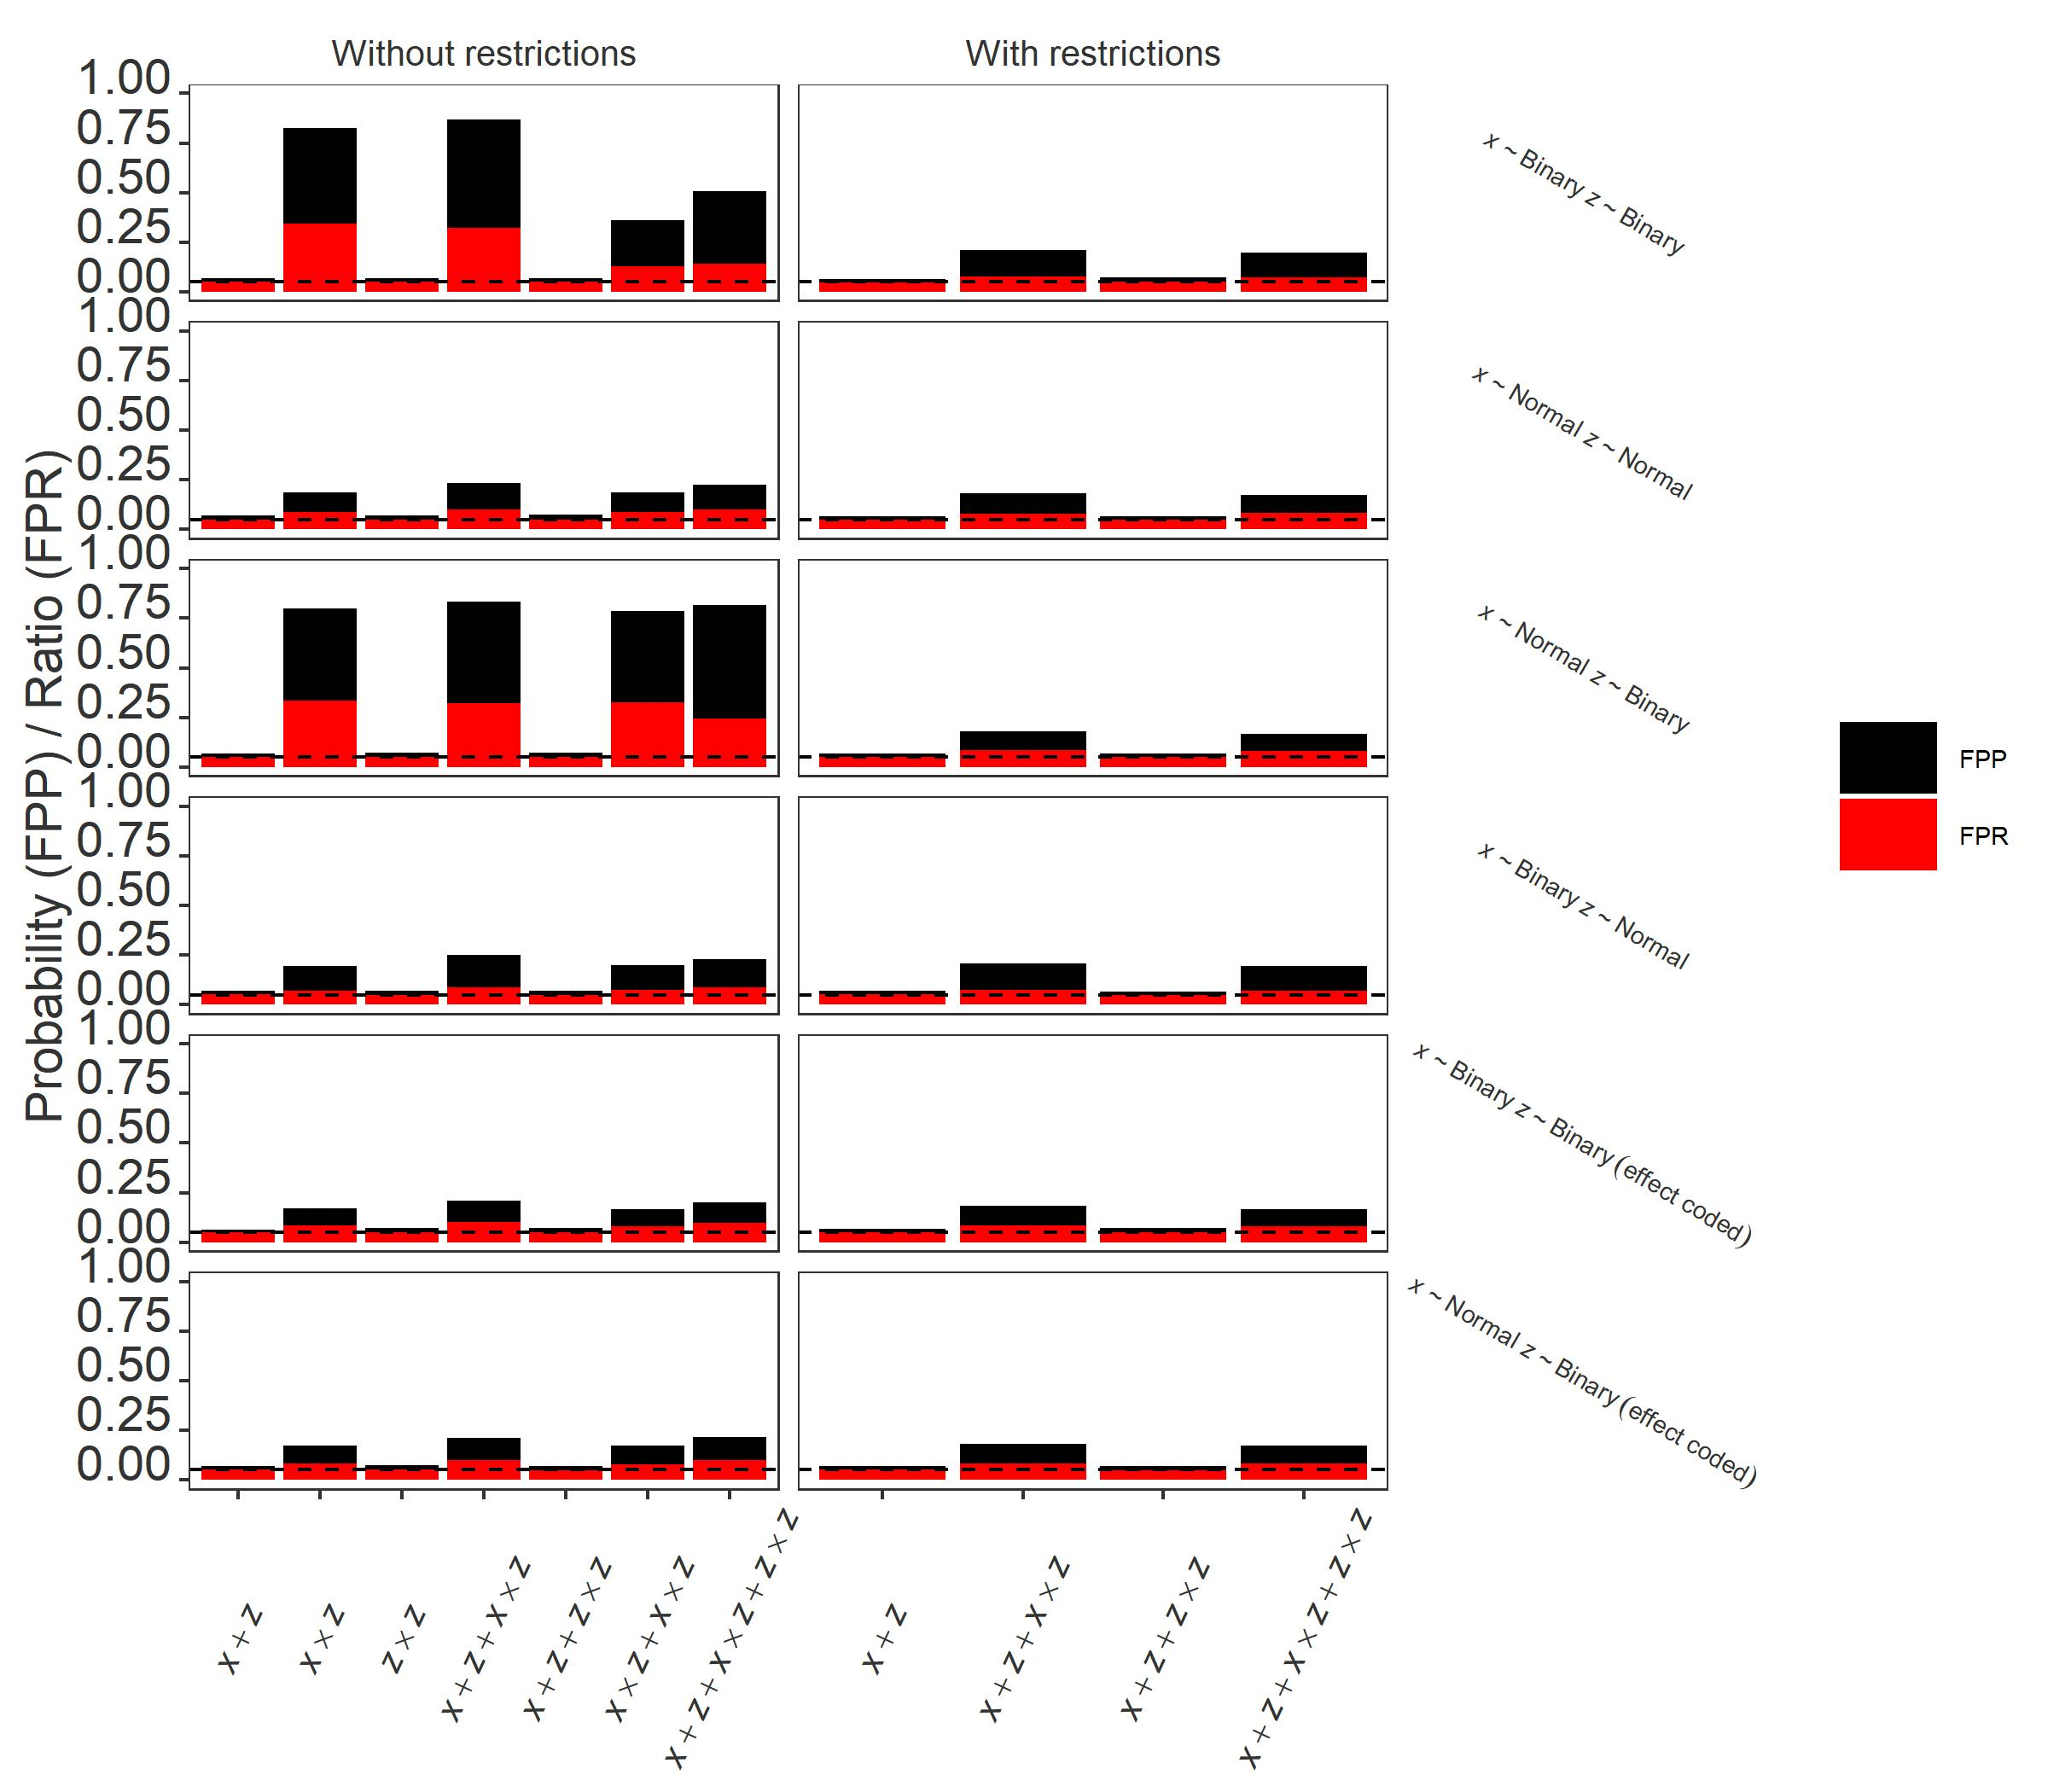
\includegraphics[width=1\textwidth]{R/Analysis/Result/Figures/Figure1ASI.jpeg}
\centering
\caption{The false-positive probability and false-positive ratio given different model sets, the presence of main effects when having interactions (i.e., Without restrictions or With restrictions) and different distributions of the variable of interest and covariates. The figure includes the two other cases compared to the main article i.e., when the variable of interest is binary and the covariates are continuous and the other way around. Sample size is set to 200, a correlation between the dependent variable and covariates is $\textit{r}=0.2$, no outlier criteria is used, and there are two covariates. The false-positive probability is shown in black and the false-positive ratio in red. Dashed blacked line shows the critical value, here set at 0.05. This figure adds the two other cases not shown in Figure \ref{fig:mainfigure1}.}
\label{fig:appfigure1}
\end{figure}

\begin{landscape}
\begin{figure}[ht!]
%\figuretitle{Effect of increasing the correlation between the dependent variable and the covariates}
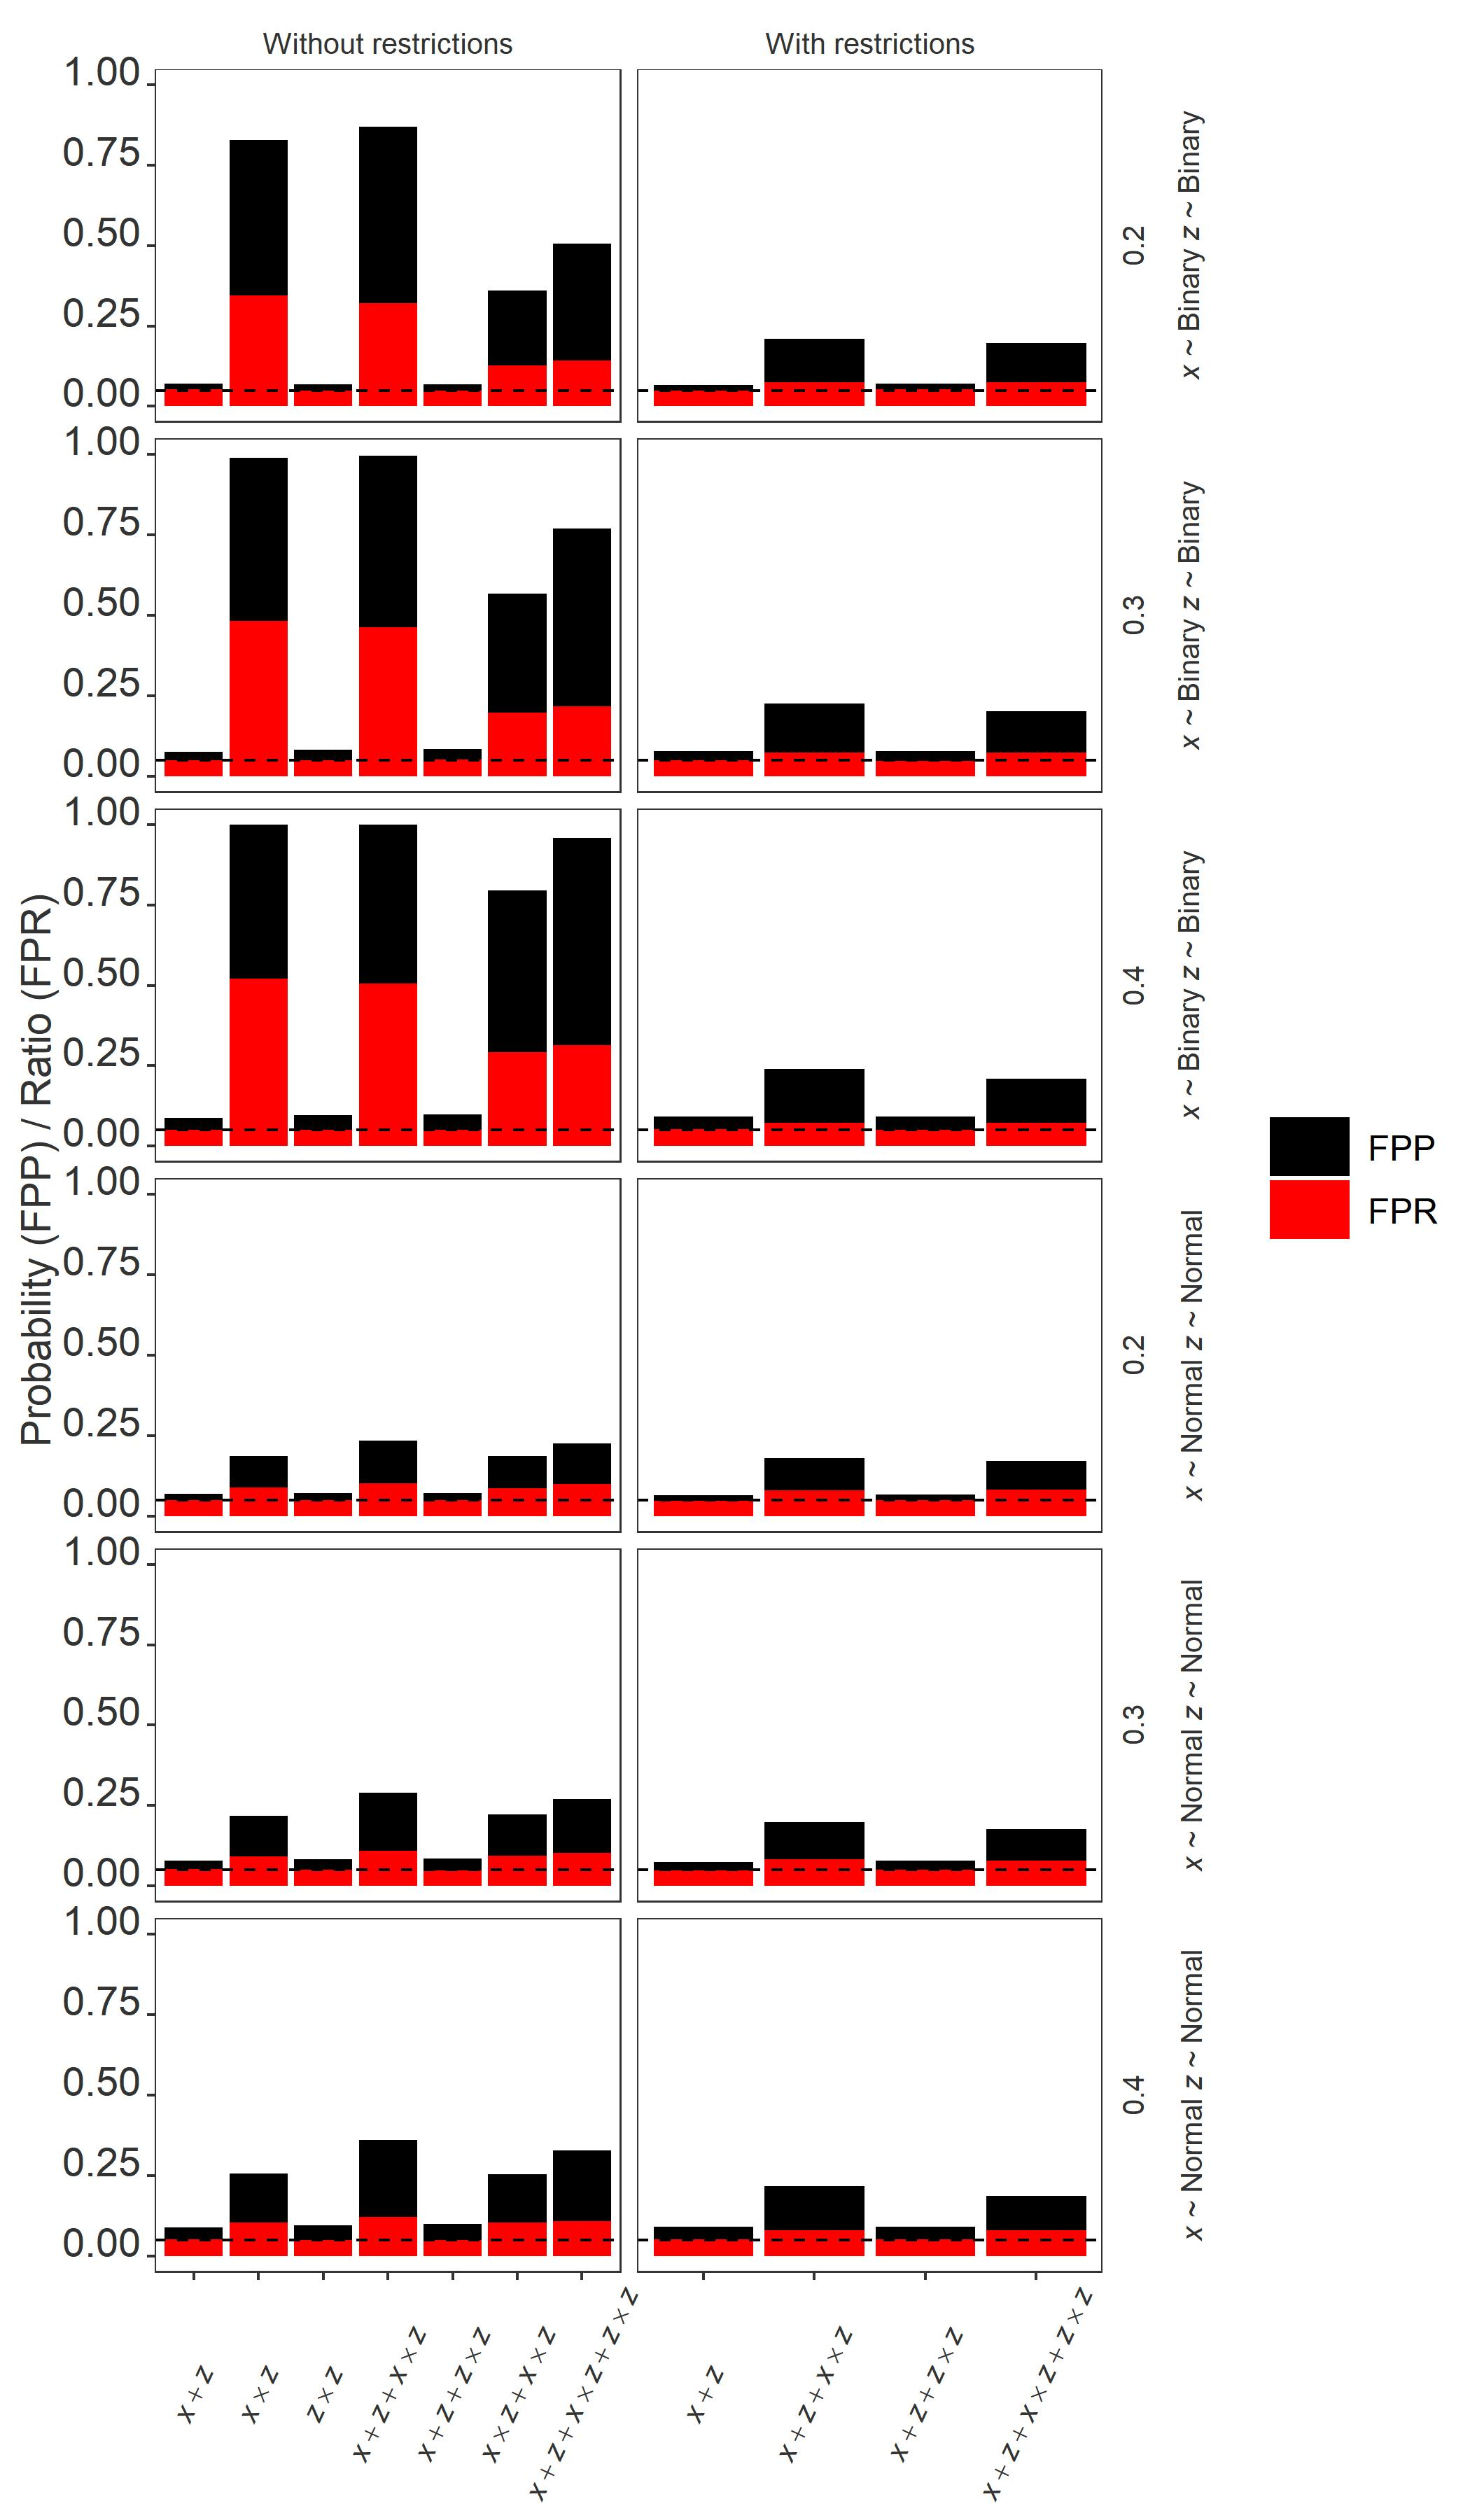
\includegraphics[scale=0.65]{R/Analysis/Result/Figures/Figure2SI.jpeg}
\centering
\caption{False-positive probability and false-positive ratio for different levels of correlation between the dependent variable and covariates ranging from  $\textit{r}=0.2$ to  $\textit{r}=0.4$. Black denotes the false-positive probability and red denotes the false-positive ratio. Dashed blacked line shows the critical value, here set at 0.05. The description of the figure is otherwise the same as for Figure \ref{fig:appfigure1}.}
\label{fig:appfigure2}
\end{figure}
\end{landscape}


\begin{figure}[ht!]
%\figuretitle{Effect of using several dependent variables}
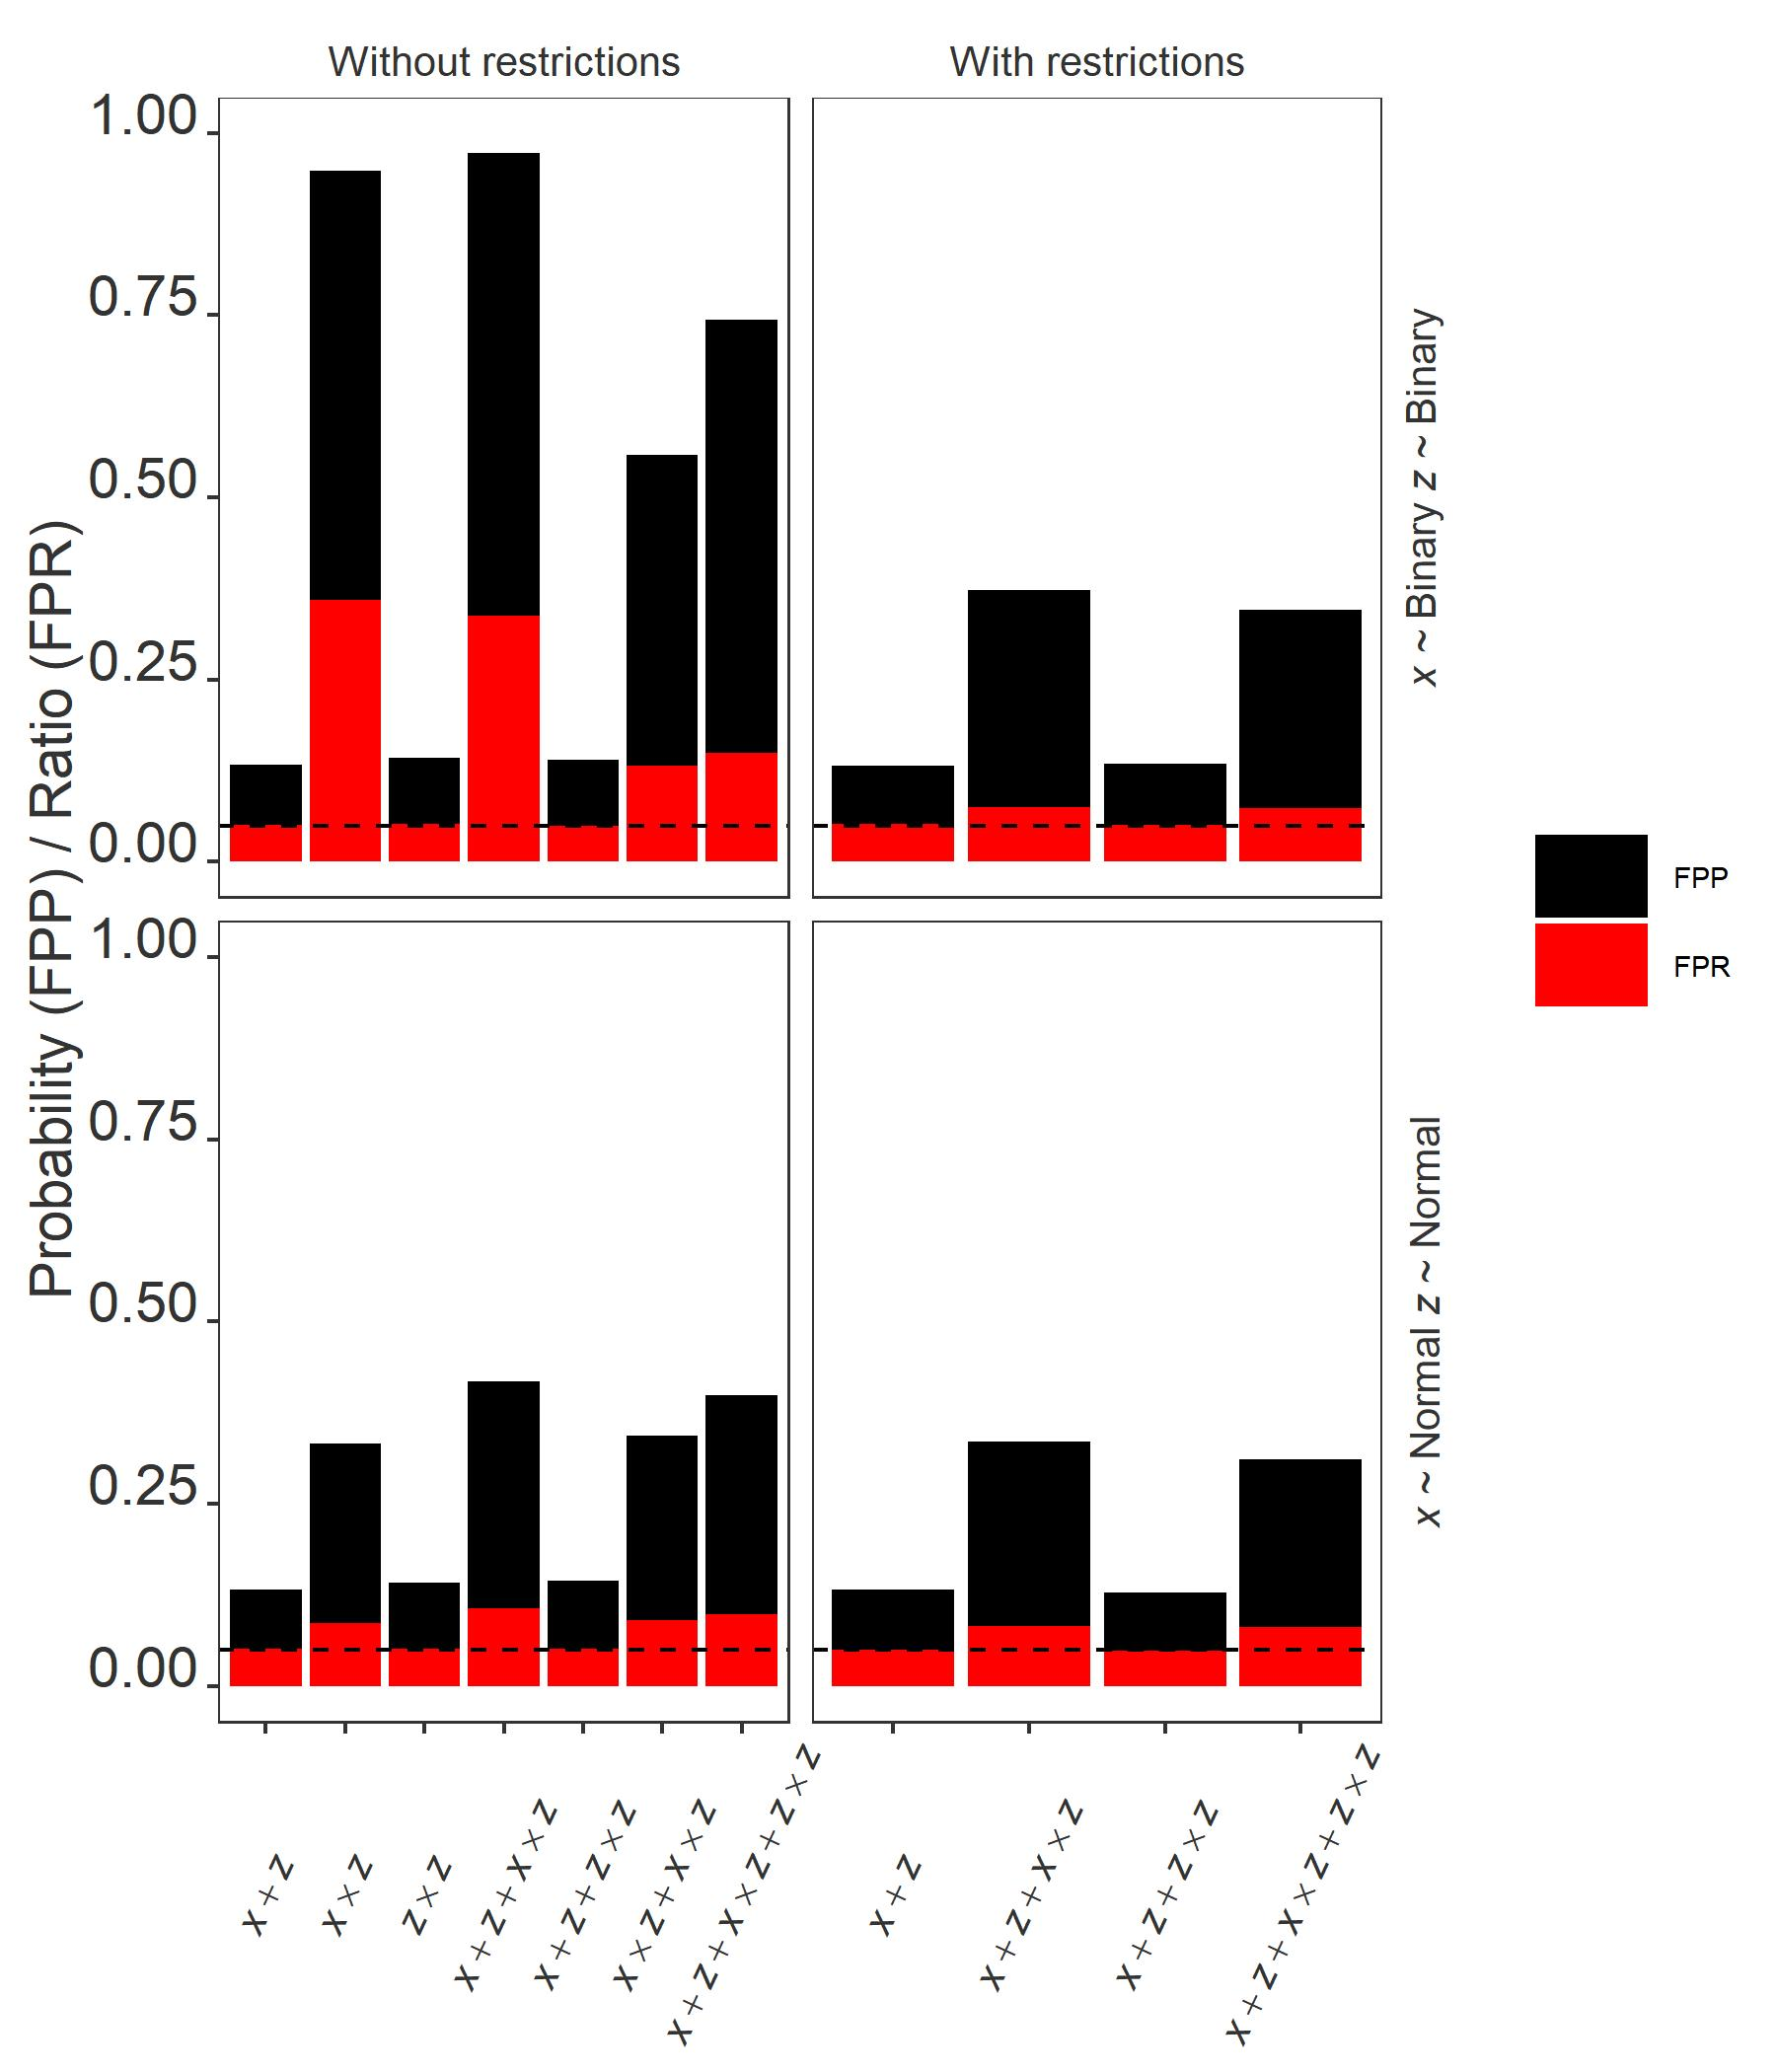
\includegraphics[width=0.8\textwidth]{R/Analysis/Result/Figures/Figure3SI.jpeg}
\centering
\caption{False-positive probability and false-positive ratio when using two dependent variables and the average of the two (three dependent variables in total). The correlation between the dependent variables is set to  $\textit{r}=0.5$ with the correlation between the dependent variables and covariates still at  $\textit{r}=0.2$. Black denotes the false-positive probability and red denotes the false-positive ratio. Dashed blacked line shows the critical value, here set at 0.05. The description of the figure is otherwise the same as for Figure \ref{fig:appfigure1}.}
\label{fig:appfigure3}
\end{figure}


\begin{figure}[ht!]
%\figuretitle{Effect of using multiple outlier criteria}
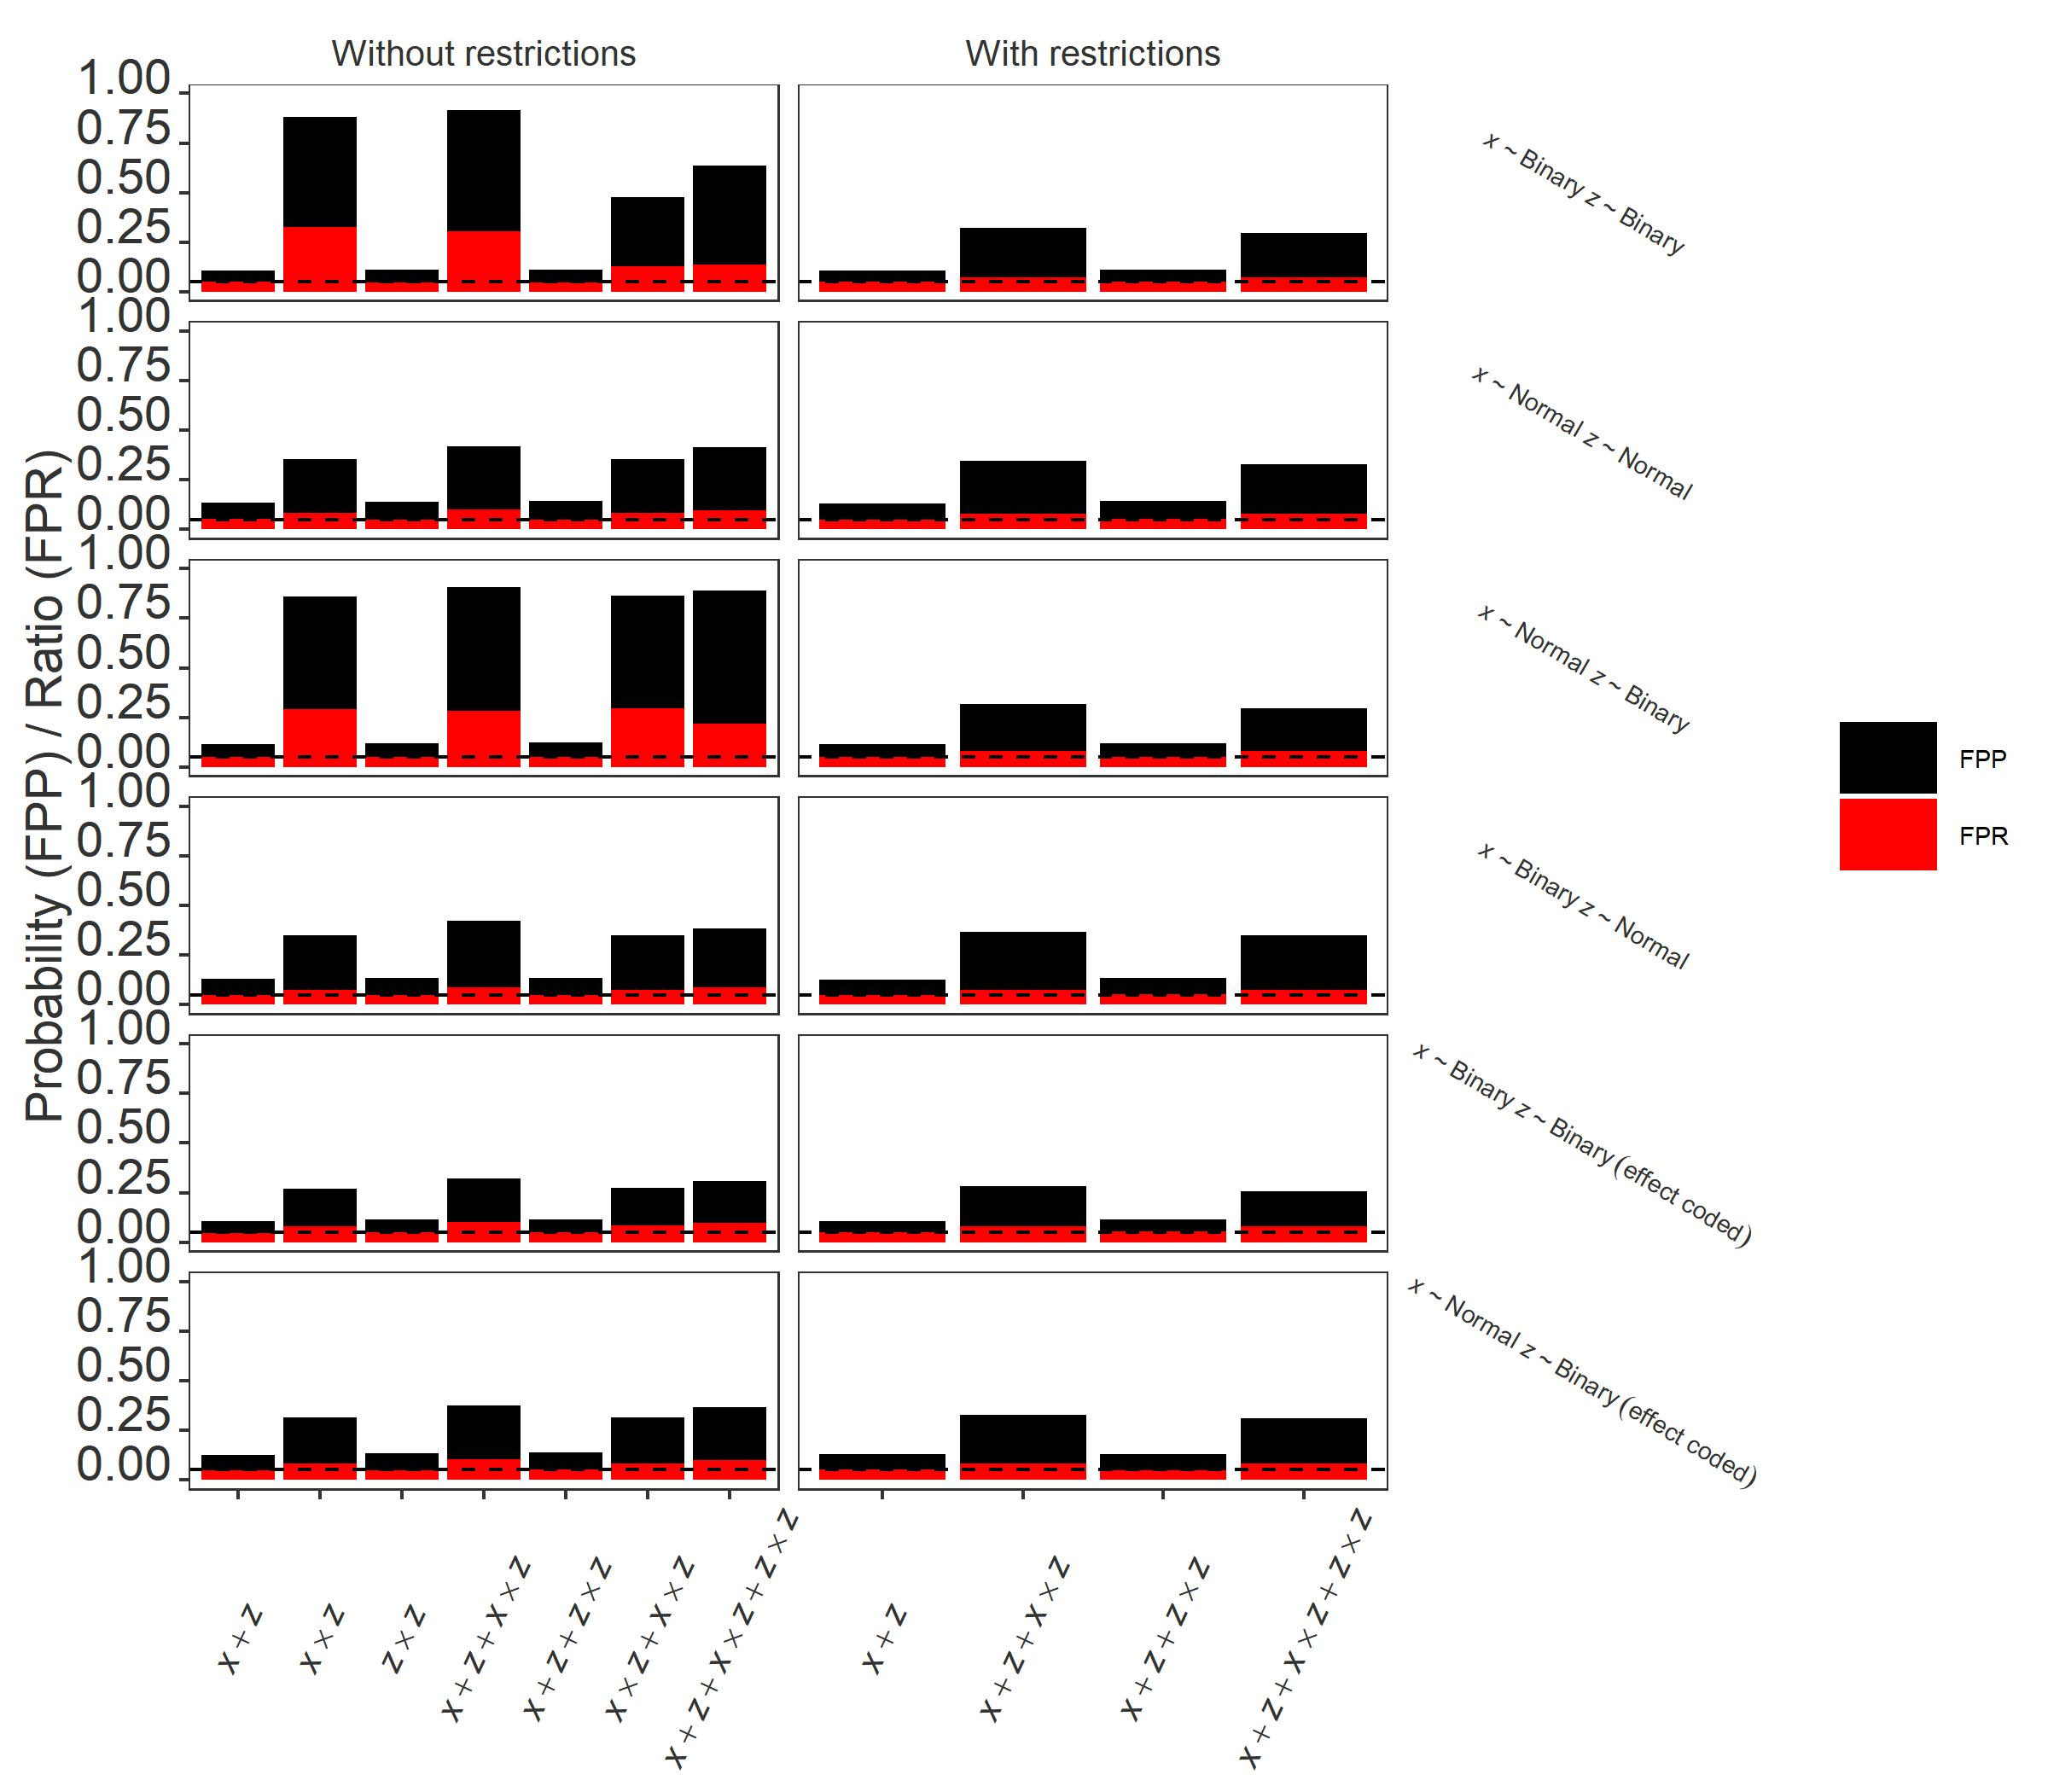
\includegraphics[width=1\textwidth]{R/Analysis/Result/Figures/Figure1BSI.jpeg}
\centering
\caption{False-positive probability and false-positive ratio when using multiple outlier criteria. Black denotes the false-positive probability and red denotes the false-positive ratio. Dashed blacked line shows the critical value, here set at 0.05. This figure adds the two other cases not shown in Figure \ref{fig:mainfigure3}. Otherwise, the description of the figure is the same as for Figure \ref{fig:appfigure1}.
}
\label{fig:appfigure4}
\end{figure}

\begin{figure}[ht!]
%\figuretitle{Effect of using three covariates}
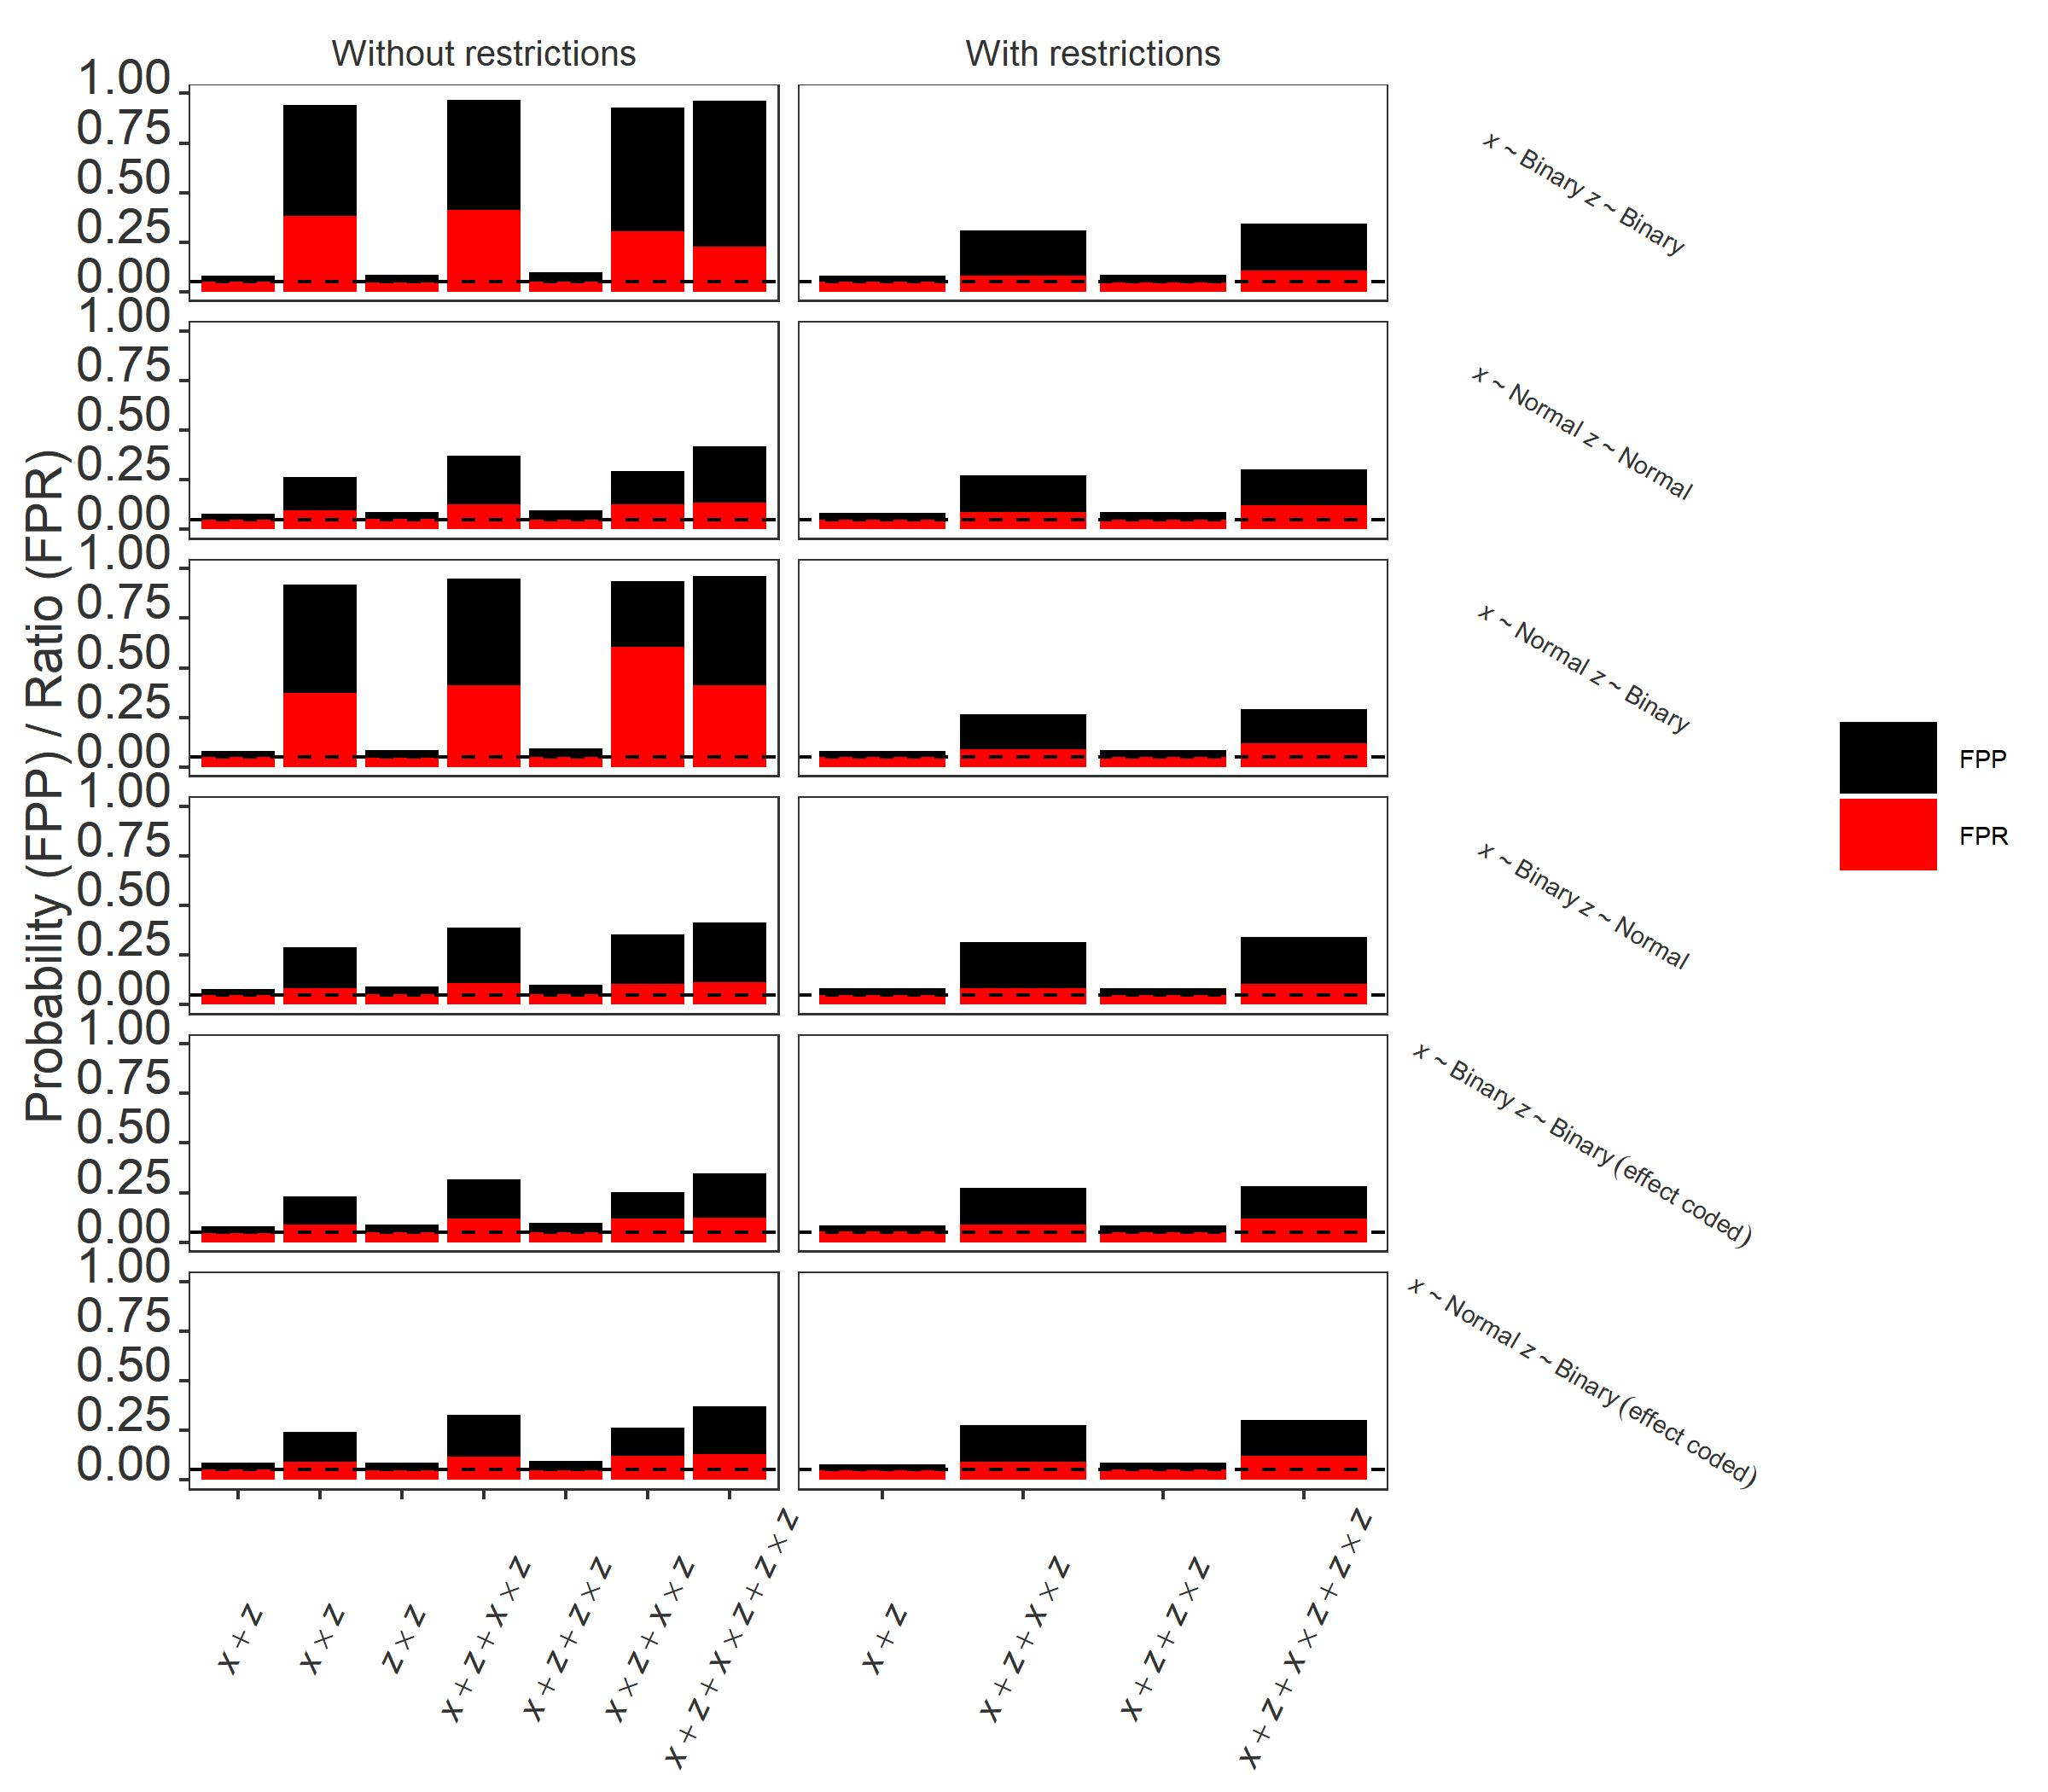
\includegraphics[width=1\textwidth]{R/Analysis/Result/Figures/Figure1CSI.jpeg}
\centering
\caption{False-positive probability and false-positive ratio when using three covariates instead of two as in the base line model. Black denotes the false-positive probability and red denotes the false-positive ratio. Dashed blacked line shows the critical value, here set at 0.05. This figure adds the two other cases not shown in Figure \ref{fig:mainfigure2}. Otherwise, the description of the figure is the same as for Figure \ref{fig:appfigure1}.
}
\label{fig:appfigure5}
\end{figure}

\begin{landscape}
\begin{figure}[ht!]
%\figuretitle{Effect of increasing the sample size}
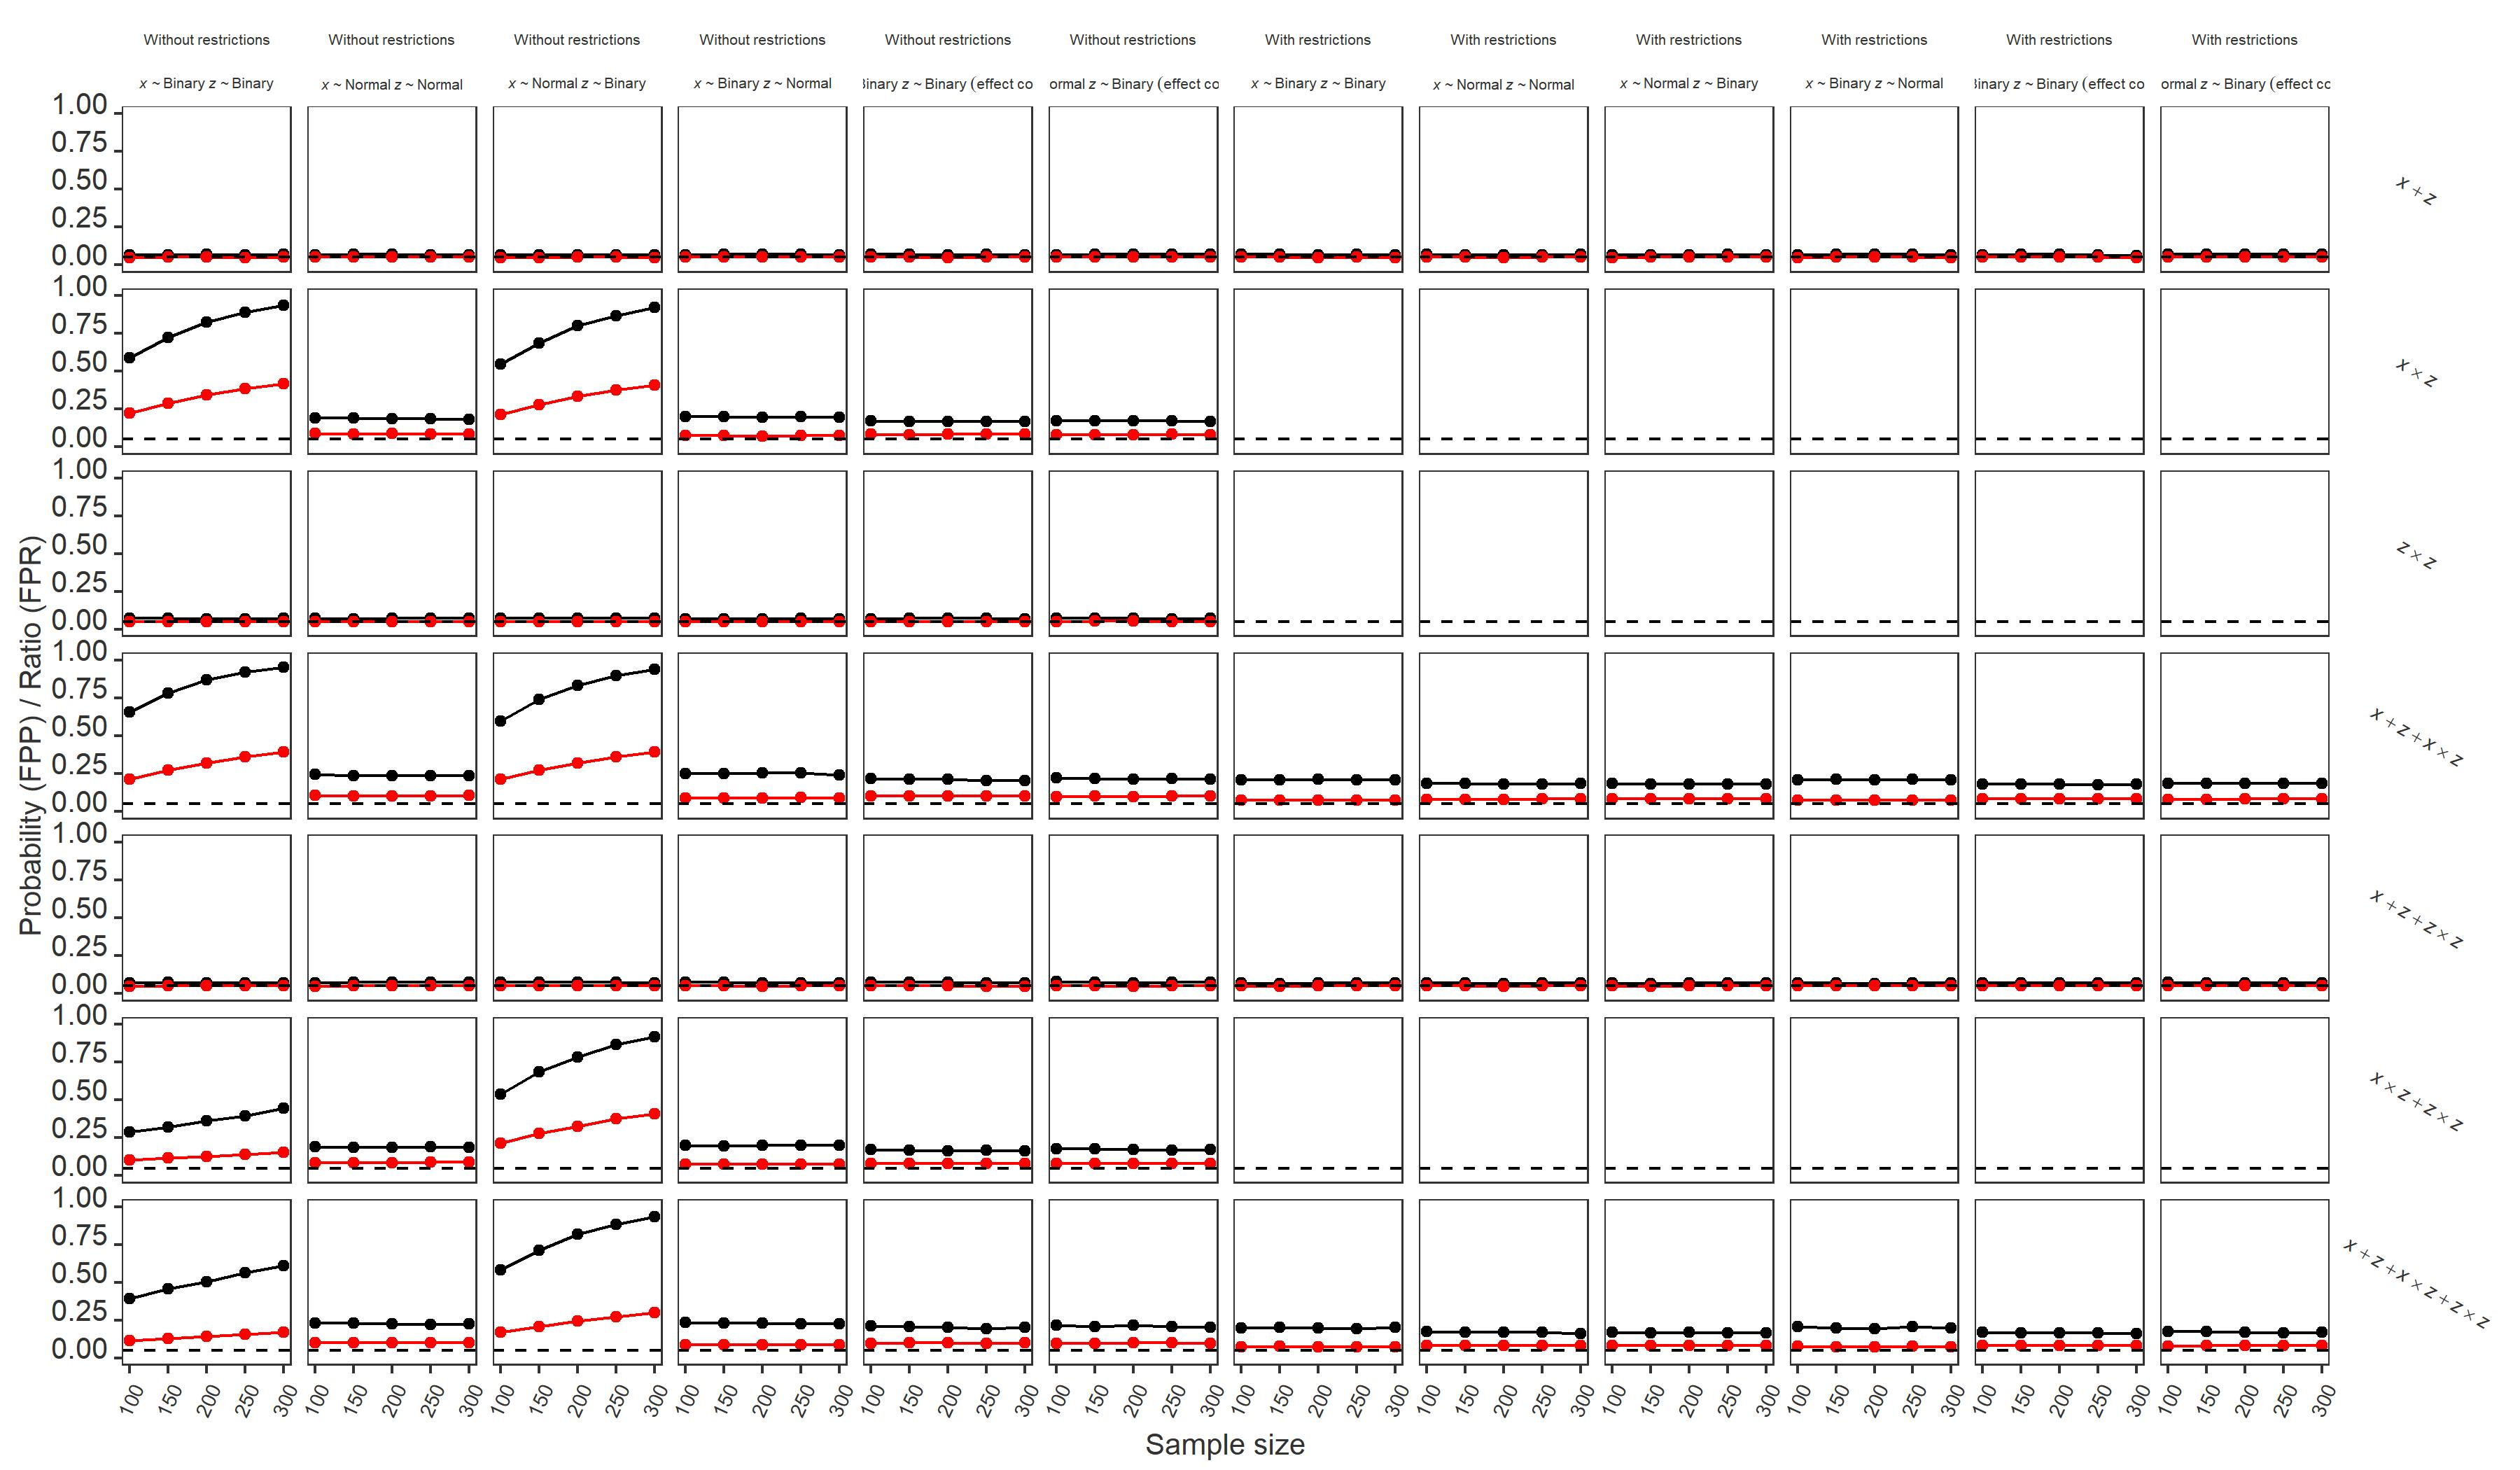
\includegraphics[scale=0.75]{R/Analysis/Result/Figures/Figure1DSI.jpeg}
\centering
\caption{Effect of increasing sample size for each model set and all combinations of data distributions (i.e., binary and normal). Black denotes the false-positive probability and red denotes the false-positive ratio. Dashed blacked line shows the critical value, here set at 0.05. This figure adds the two other cases not shown in Figure \ref{fig:mainfigure4}. Otherwise, the description of the figure is the same as for Figure \ref{fig:appfigure1}. 
}
\label{fig:appfigure6}
\end{figure}
\end{landscape}

\clearpage
\subsection{Results when using Bonferroni correction of p-values}
\label{resultBC}

In this section, we present the same analyses, but with Bonferroni correction of p-values. This means that the critical value ($\alpha$) now has a correction such that $\alpha = 0.05 / #Number~of~tests~in~each~model$. So the critical value will only be 0.05 in the case where there are no interactions between the variable of interest and covariates. The critical value is corrected for each test such that it can differ within each model set depending on how many interactions there are per model. 

\begin{figure}[ht!]
%\figuretitle{Baseline model with all the different data structures when using Bonferroni correction}
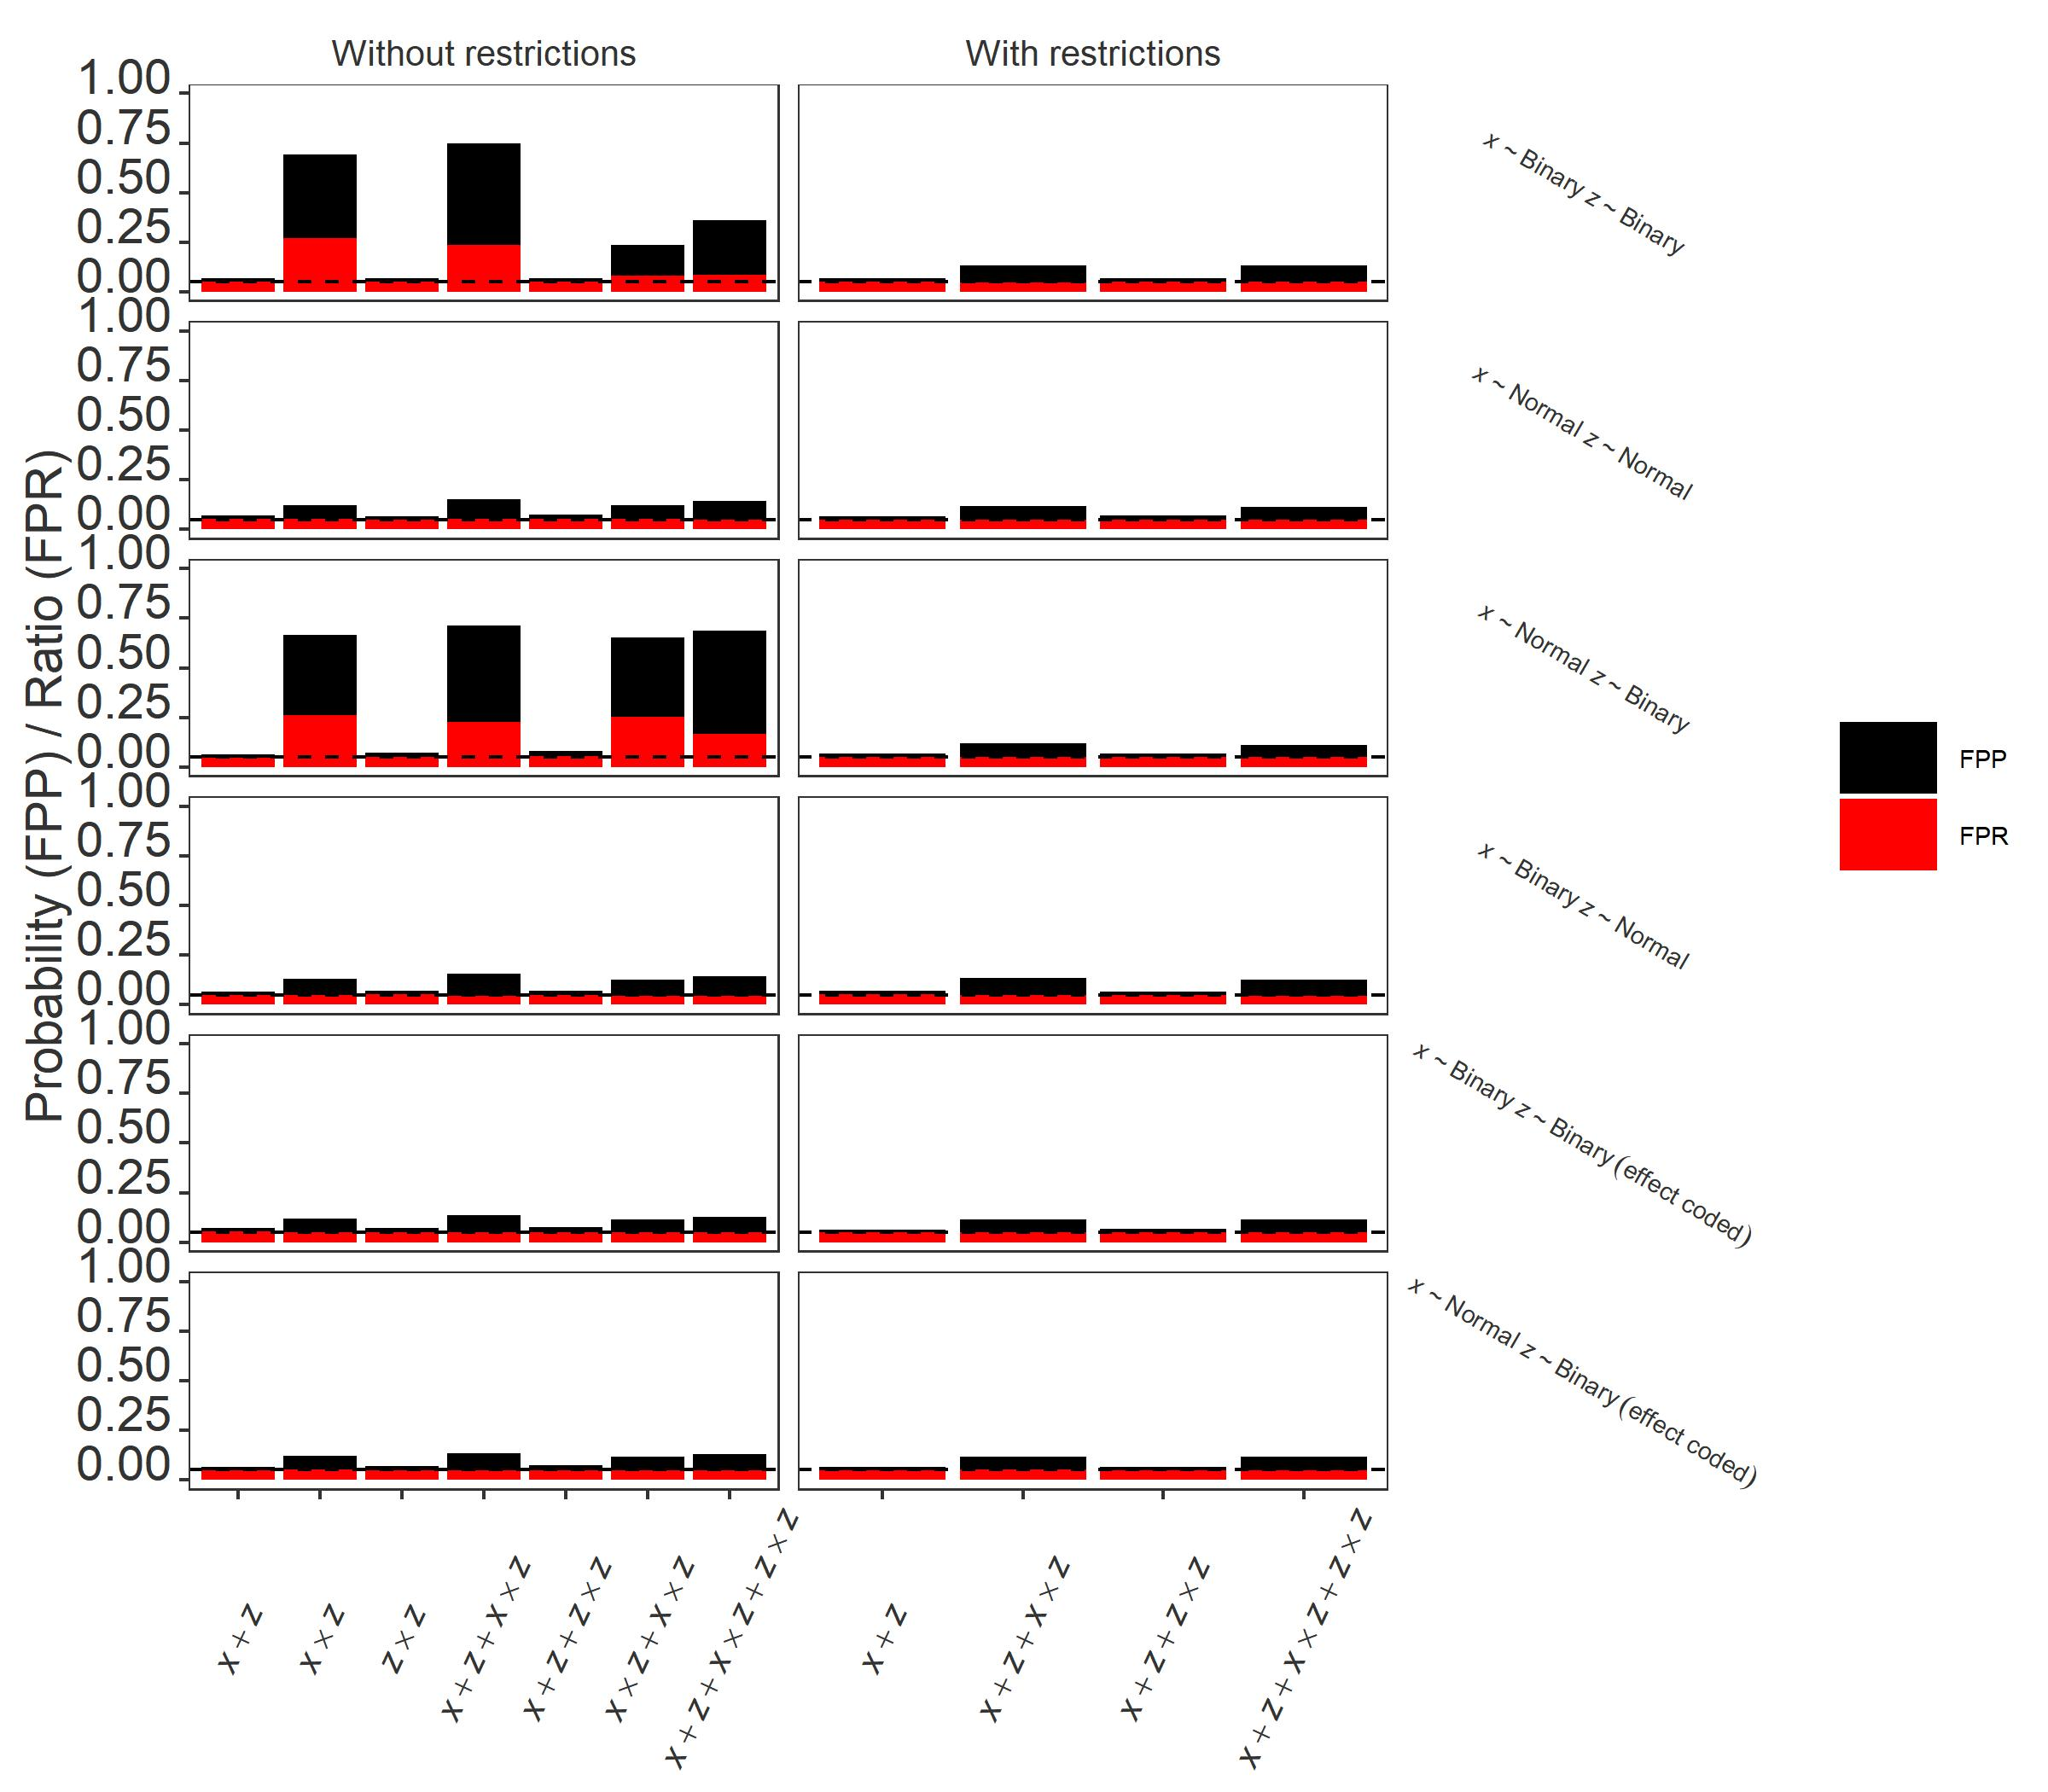
\includegraphics[width=1\textwidth]{R/Analysis/Result/Figures/Figure1ASIBon.jpeg}
\centering
\caption{The description of this figure is the same as for Figure \ref{fig:appfigure1} with the only difference being that we applied Bonferroni correction. This figure therefore shows the false-positive probability and false-positive ratio given different model sets, the presence of main effects when having interactions (i.e., Without restrictions or With restrictions), and different distributions of the variable of interest and covariates. Sample size is set to 200, a correlation between the dependent variable and covariates is $\textit{r}=0.2$, no outlier criteria is used, and there are two covariates. The false-positive probability is shown in black and false-positive ratio in red. Dashed blacked line shows the critical value, here set at 0.05. }
\label{fig:appfigure7}
\end{figure}

\begin{landscape}
\begin{figure}[ht!]
%\figuretitle{Effect of increasing the correlation between the dependent variable and the covariates when using Bonferroni correction}
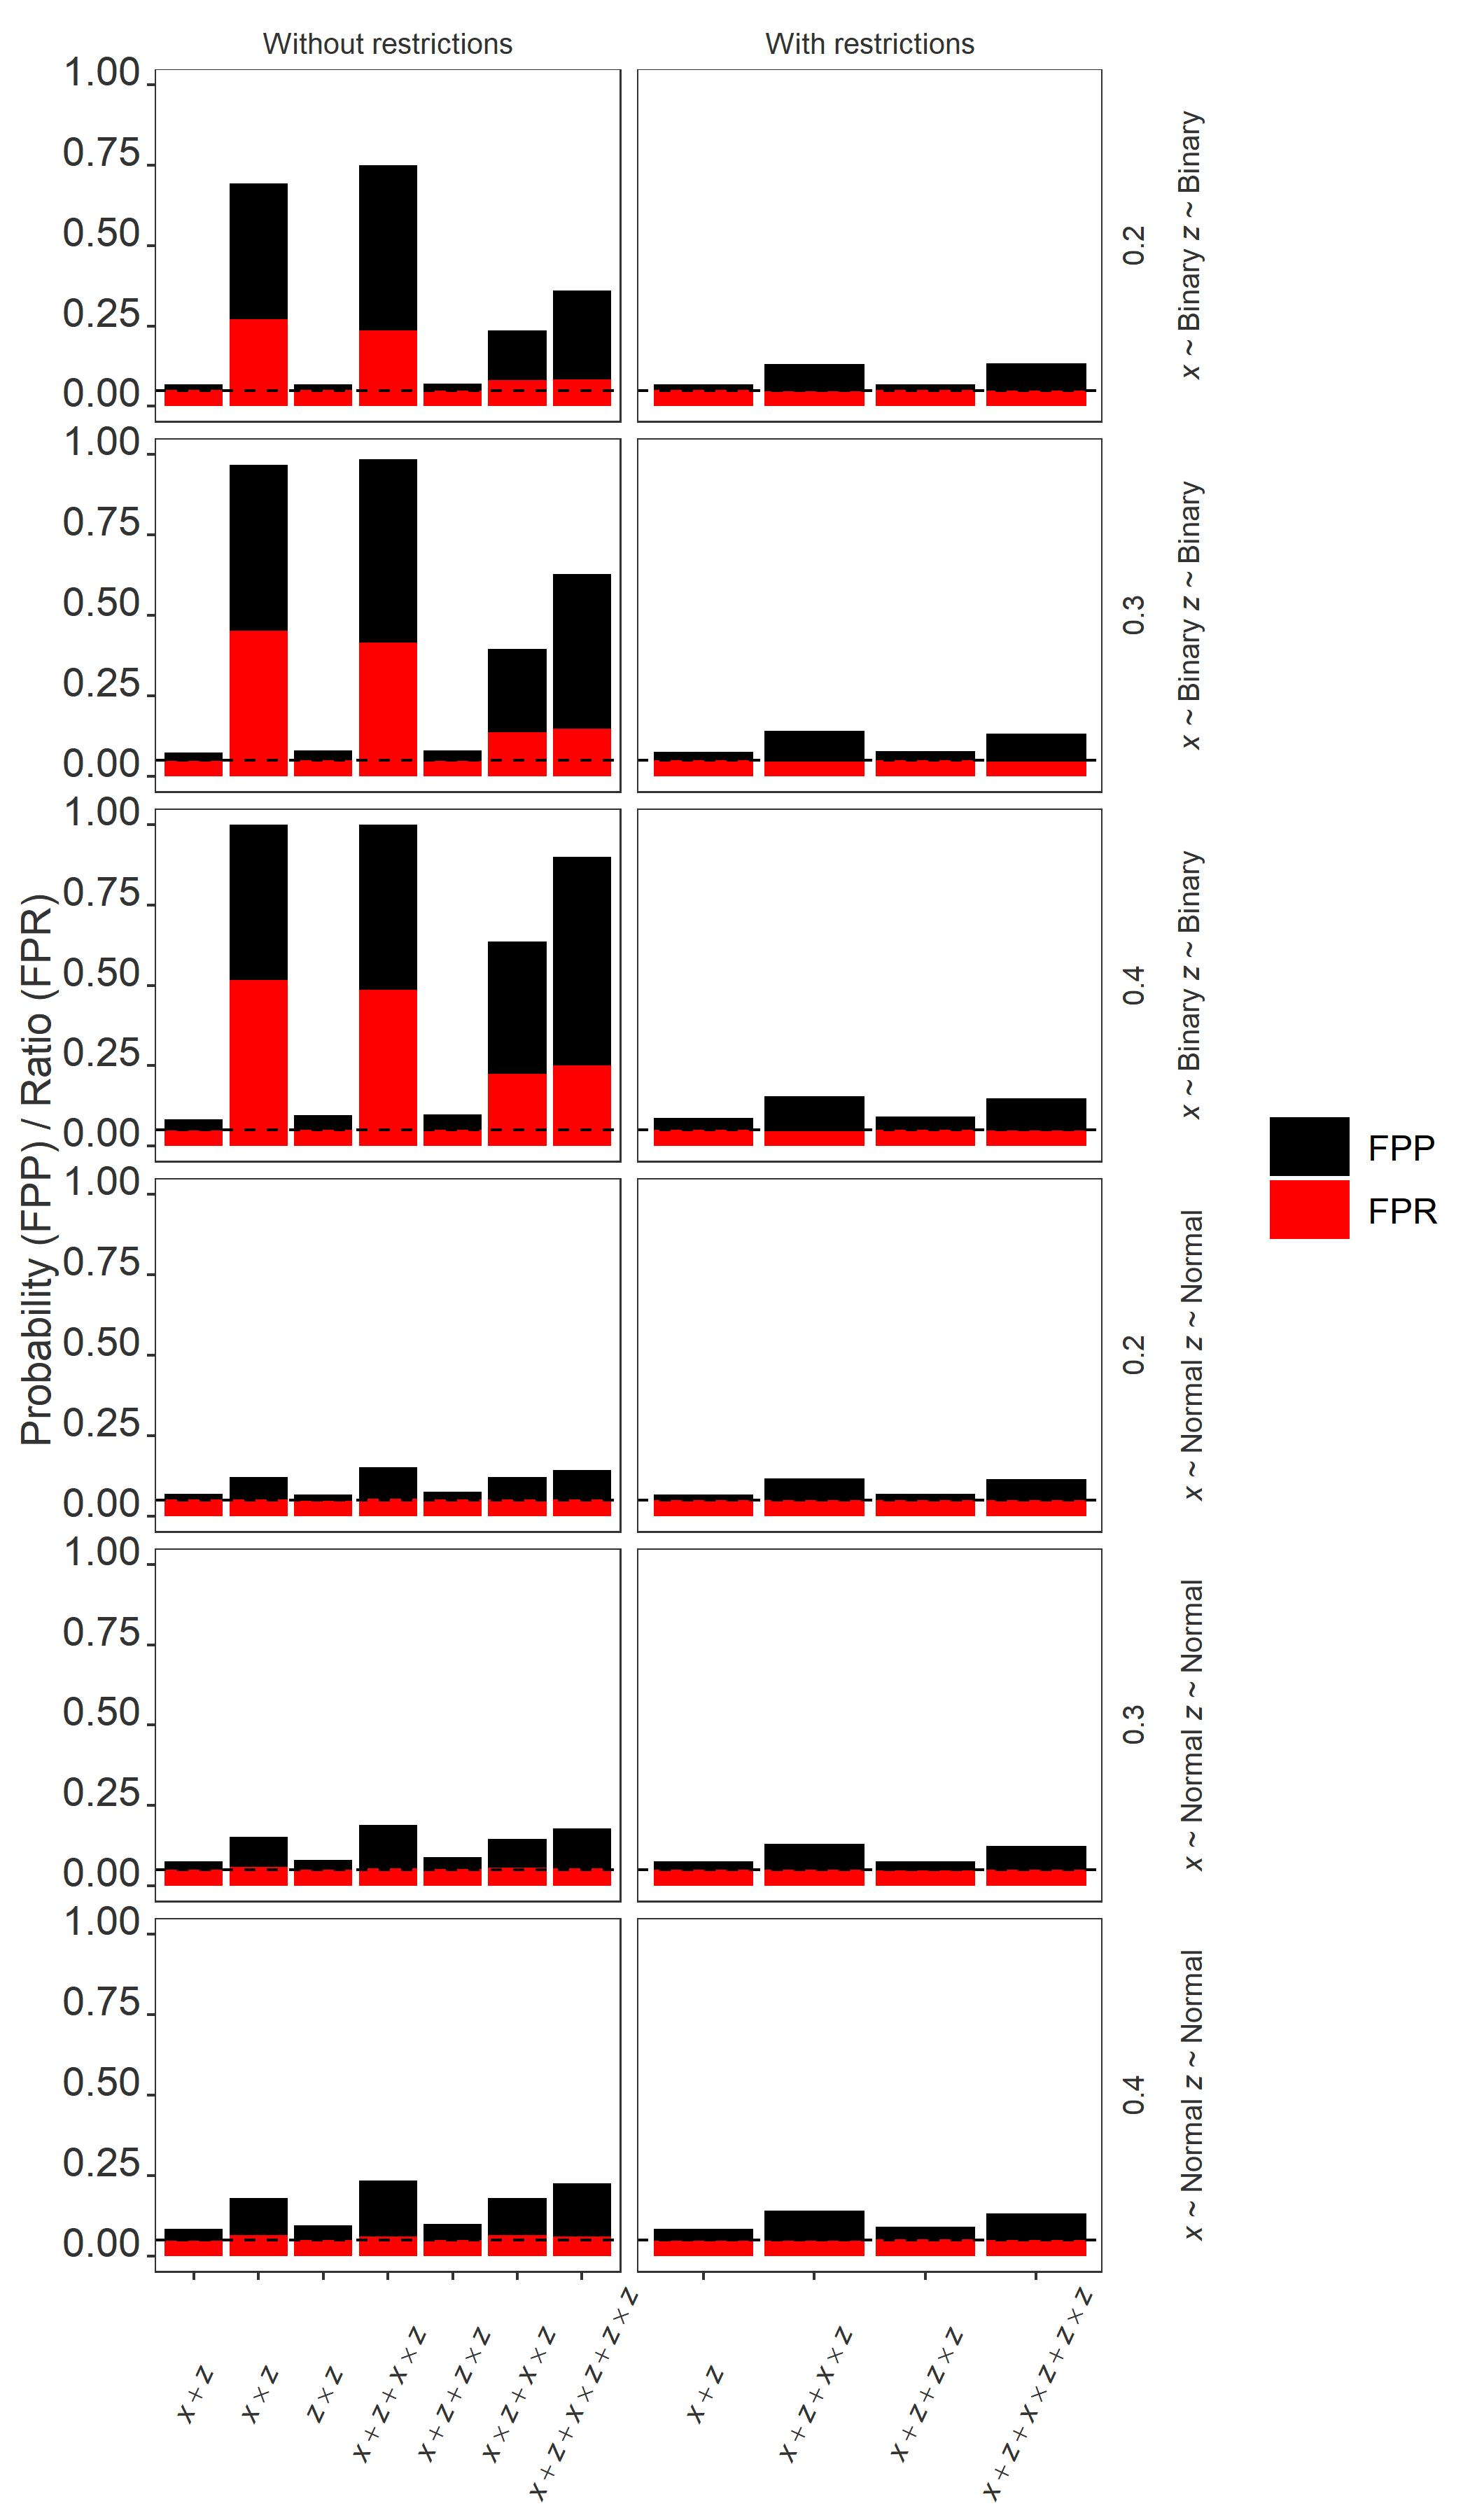
\includegraphics[scale=0.65]{R/Analysis/Result/Figures/Figure2SIBon.jpeg}
\centering
\caption{False-positive probability and false-positive ratio for different levels of correlation between the dependent variable and covariates ranging from  $\textit{r}=0.2$ to  $\textit{r}=0.4$ when using Bonferroni correction. Black denotes the false-positive probability and red denotes the false-positive ratio. Dashed blacked line shows the critical value, here set at 0.05. The description of the figure is otherwise the same as for Figure \ref{fig:appfigure7}.}
\label{fig:appfigure8}
\end{figure}
\end{landscape}



\begin{figure}[ht!]
%\figuretitle{Effect of using several dependent variables when using Bonferroni correction}
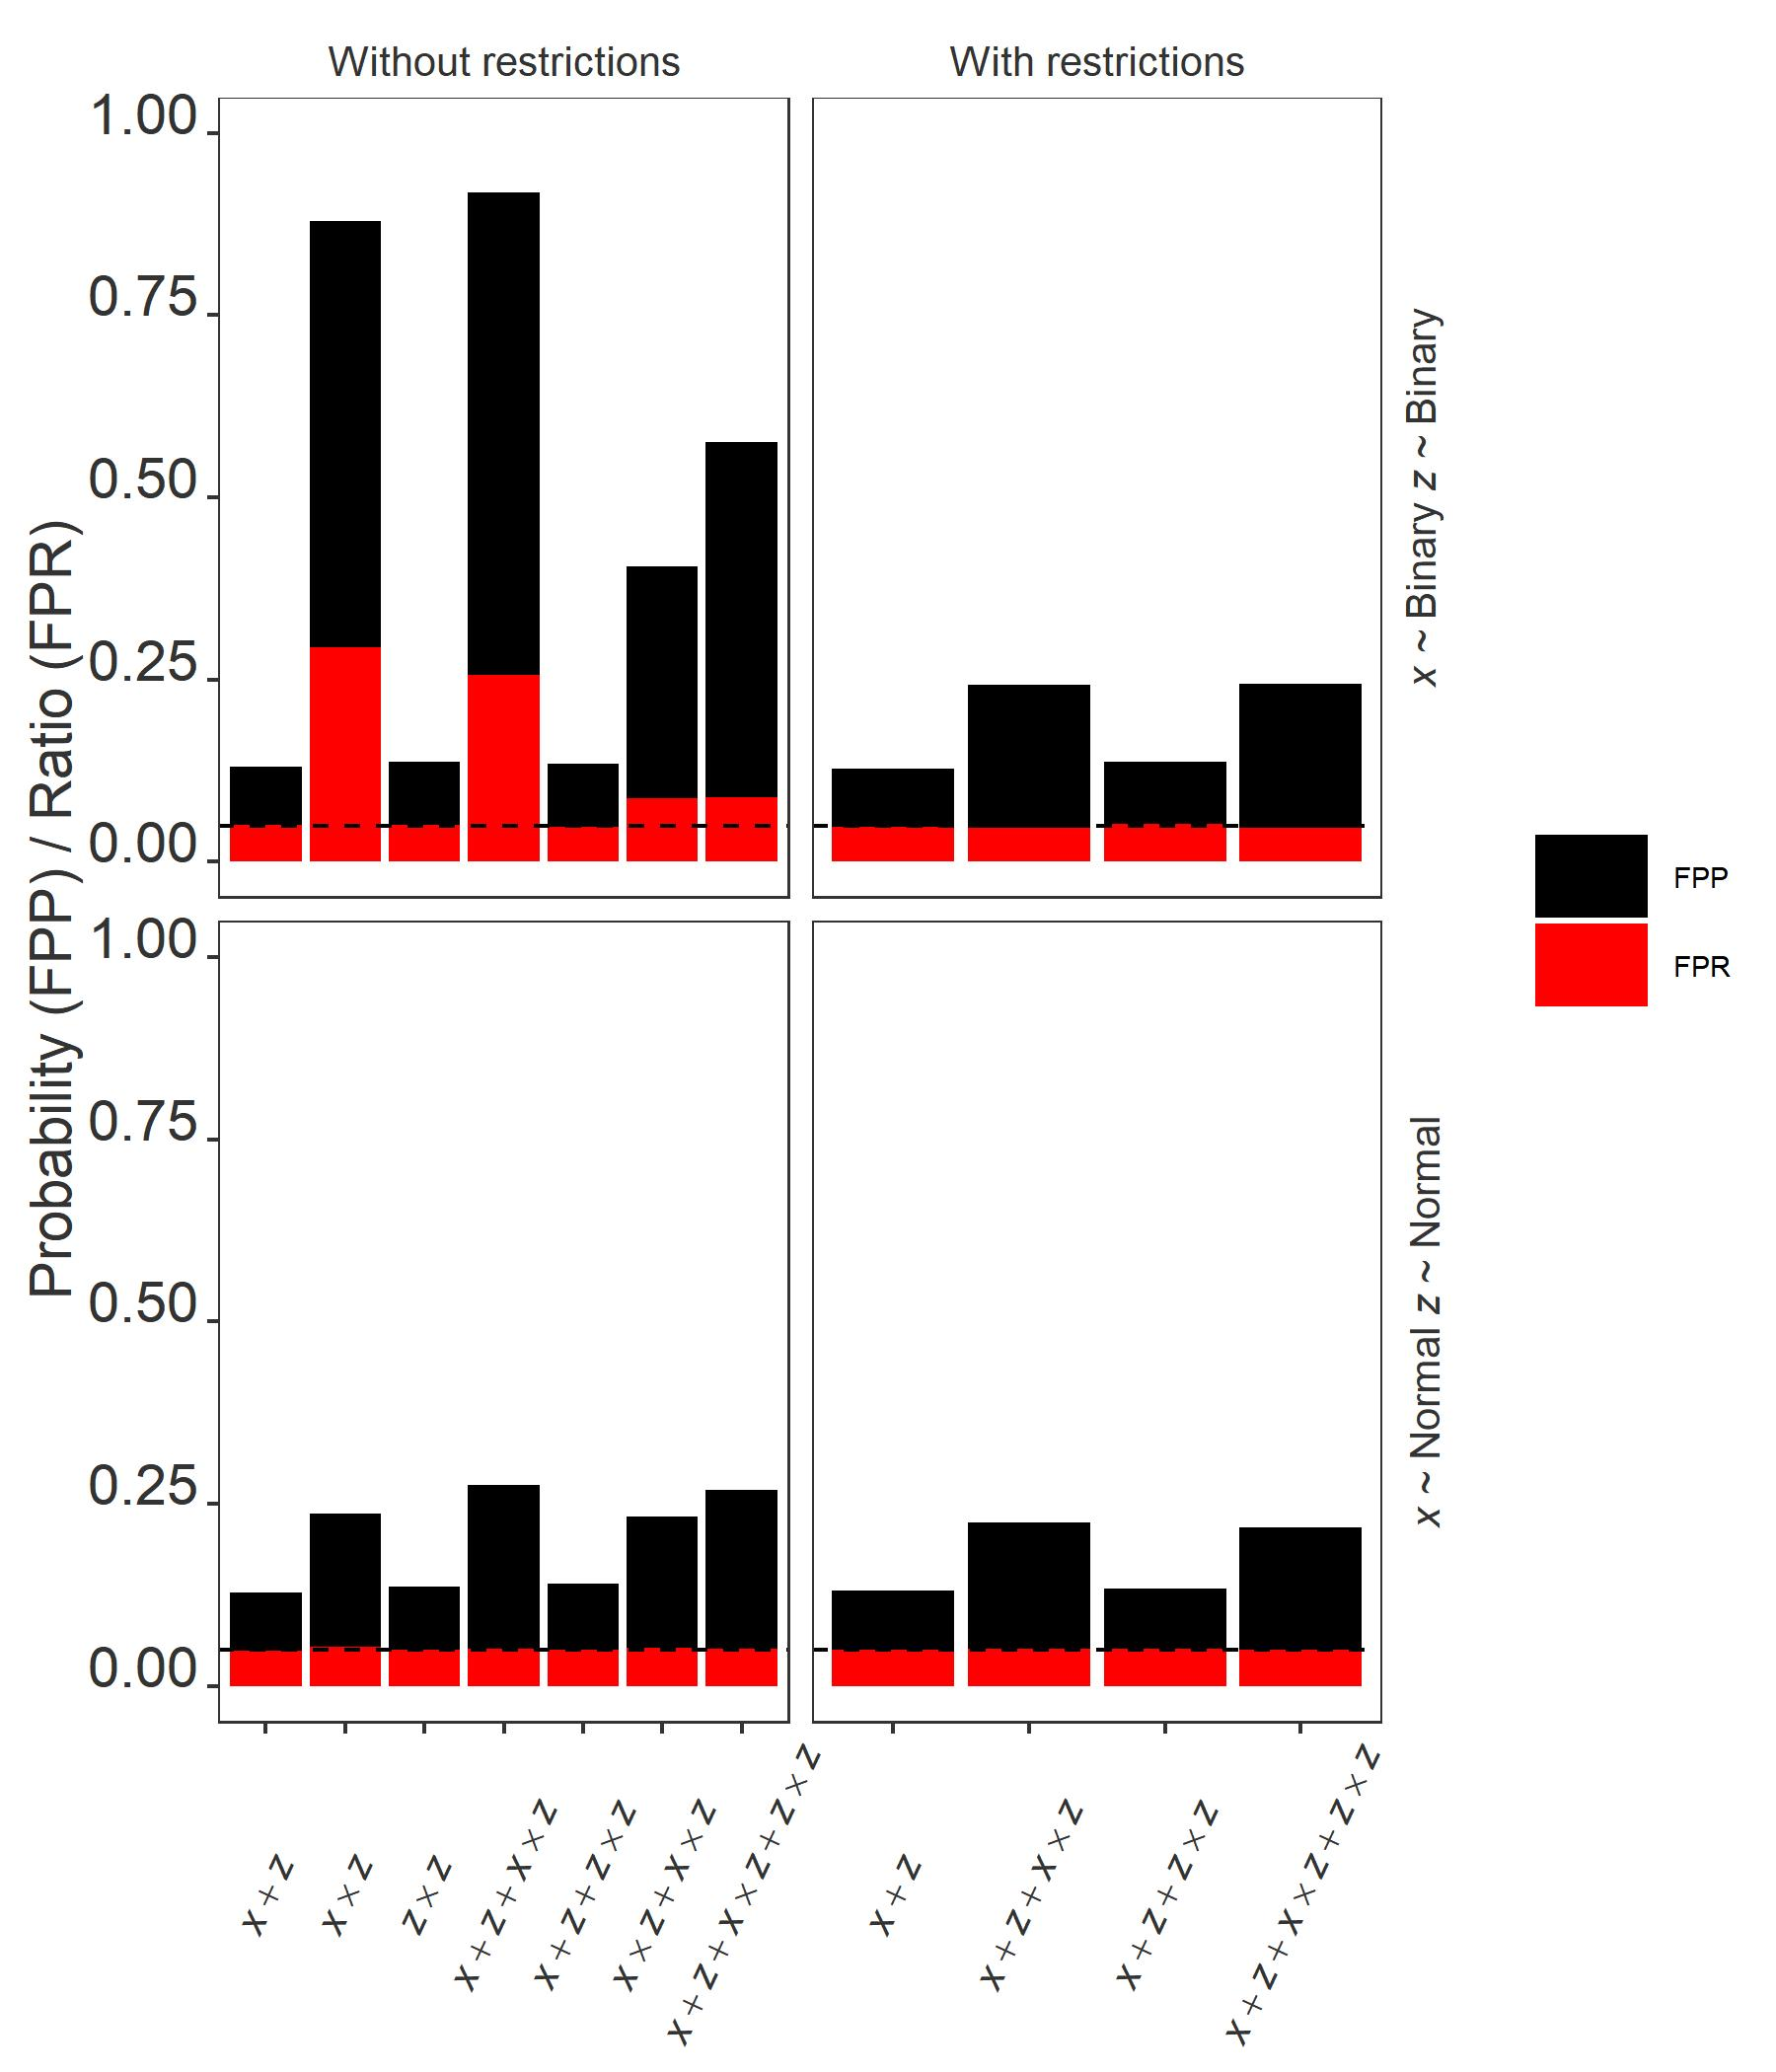
\includegraphics[width=0.8\textwidth]{R/Analysis/Result/Figures/Figure3SIBon.jpeg}
\centering
\caption{False-positive probability and false-positive ratio when using two dependent variables and the average of the two (three dependent variables in total) when using Bonferroni correction. The correlation between the dependent variables is set to  $\textit{r}=0.5$ with the correlation between the dependent variables and covariates still at  $\textit{r}=0.2$. Black denotes the false-positive probability and red denotes the false-positive ratio. Dashed blacked line shows the critical value, here set at 0.05. The description of the figure is otherwise the same as for Figure \ref{fig:appfigure7}.}
\label{fig:appfigure9}
\end{figure}


\begin{figure}[ht!]
%\figuretitle{Effect of using multiple outlier criteria when using Bonferroni correction}
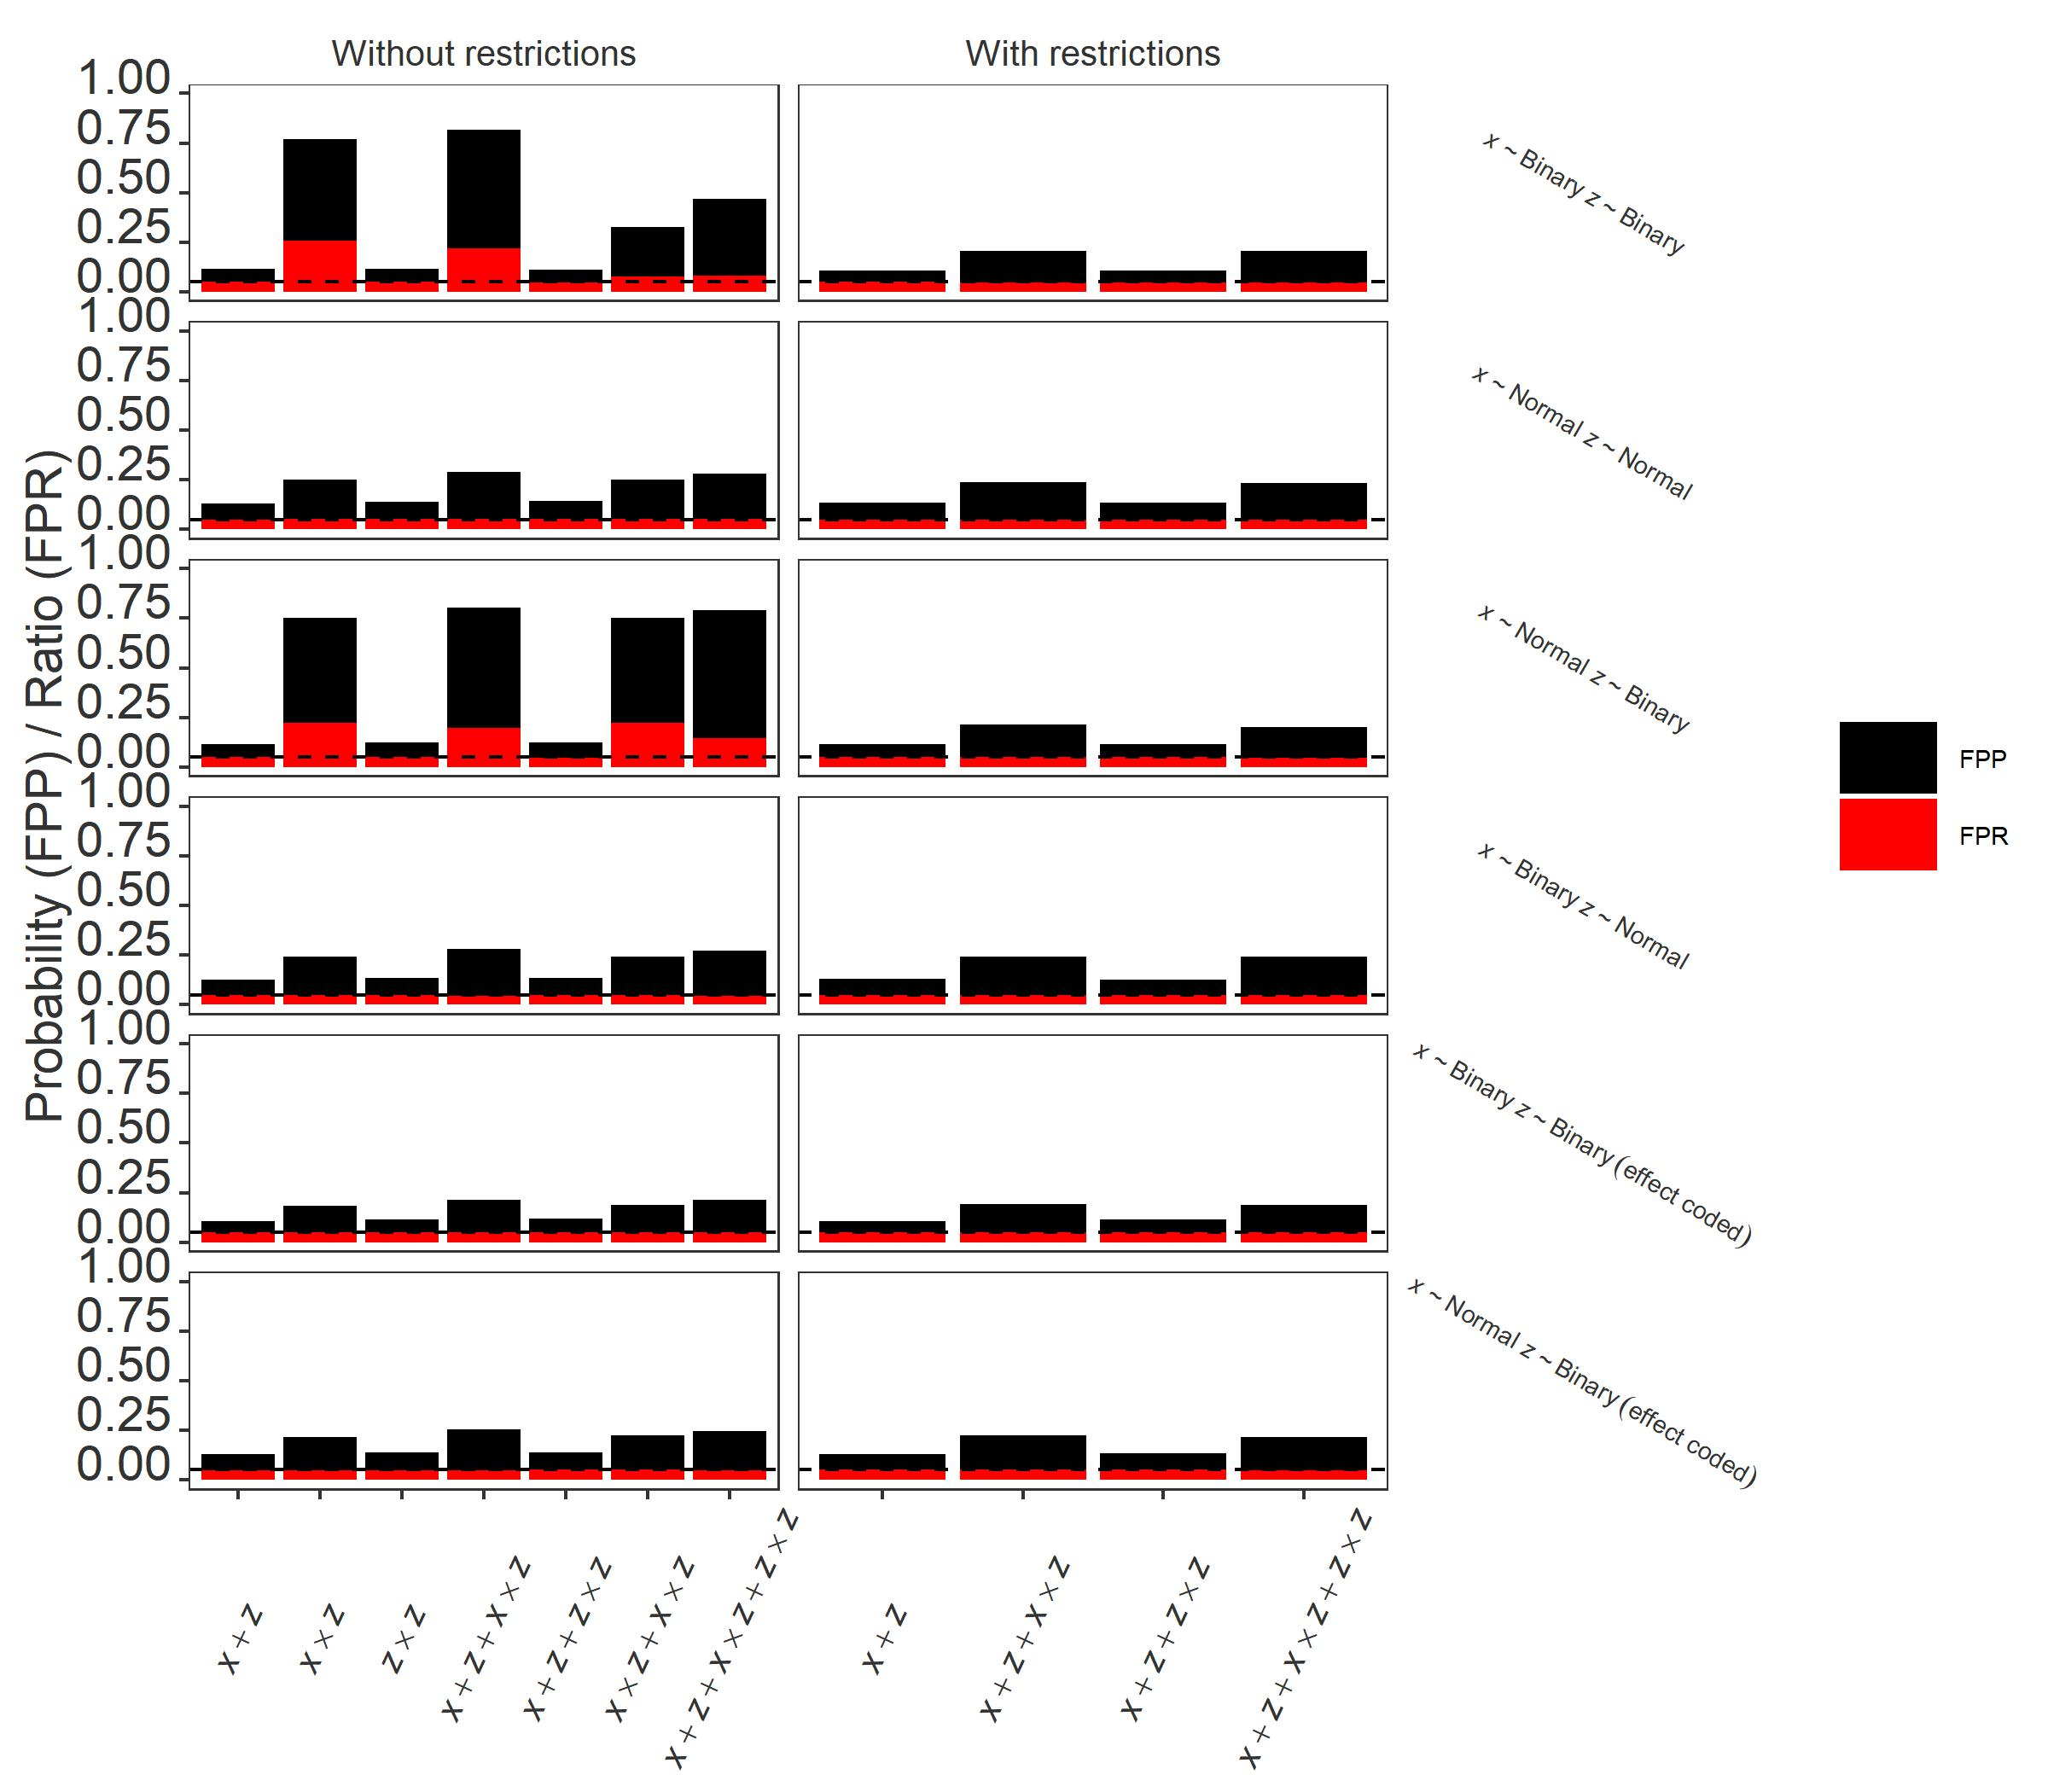
\includegraphics[width=1\textwidth]{R/Analysis/Result/Figures/Figure1BSIBon.jpeg}
\centering
\caption{False-positive probability and false-positive ratio when using multiple outlier criteria and Bonferroni correction. Black denotes the false-positive probability and red denotes the false-positive ratio. Dashed blacked line shows the critical value, here set at 0.05. The description of the figure is otherwise the same as for Figure \ref{fig:appfigure7}.
}
\label{fig:appfigure10}
\end{figure}


\begin{figure}[ht!]
%\figuretitle{Effect of using three covariates when using Bonferroni correction}
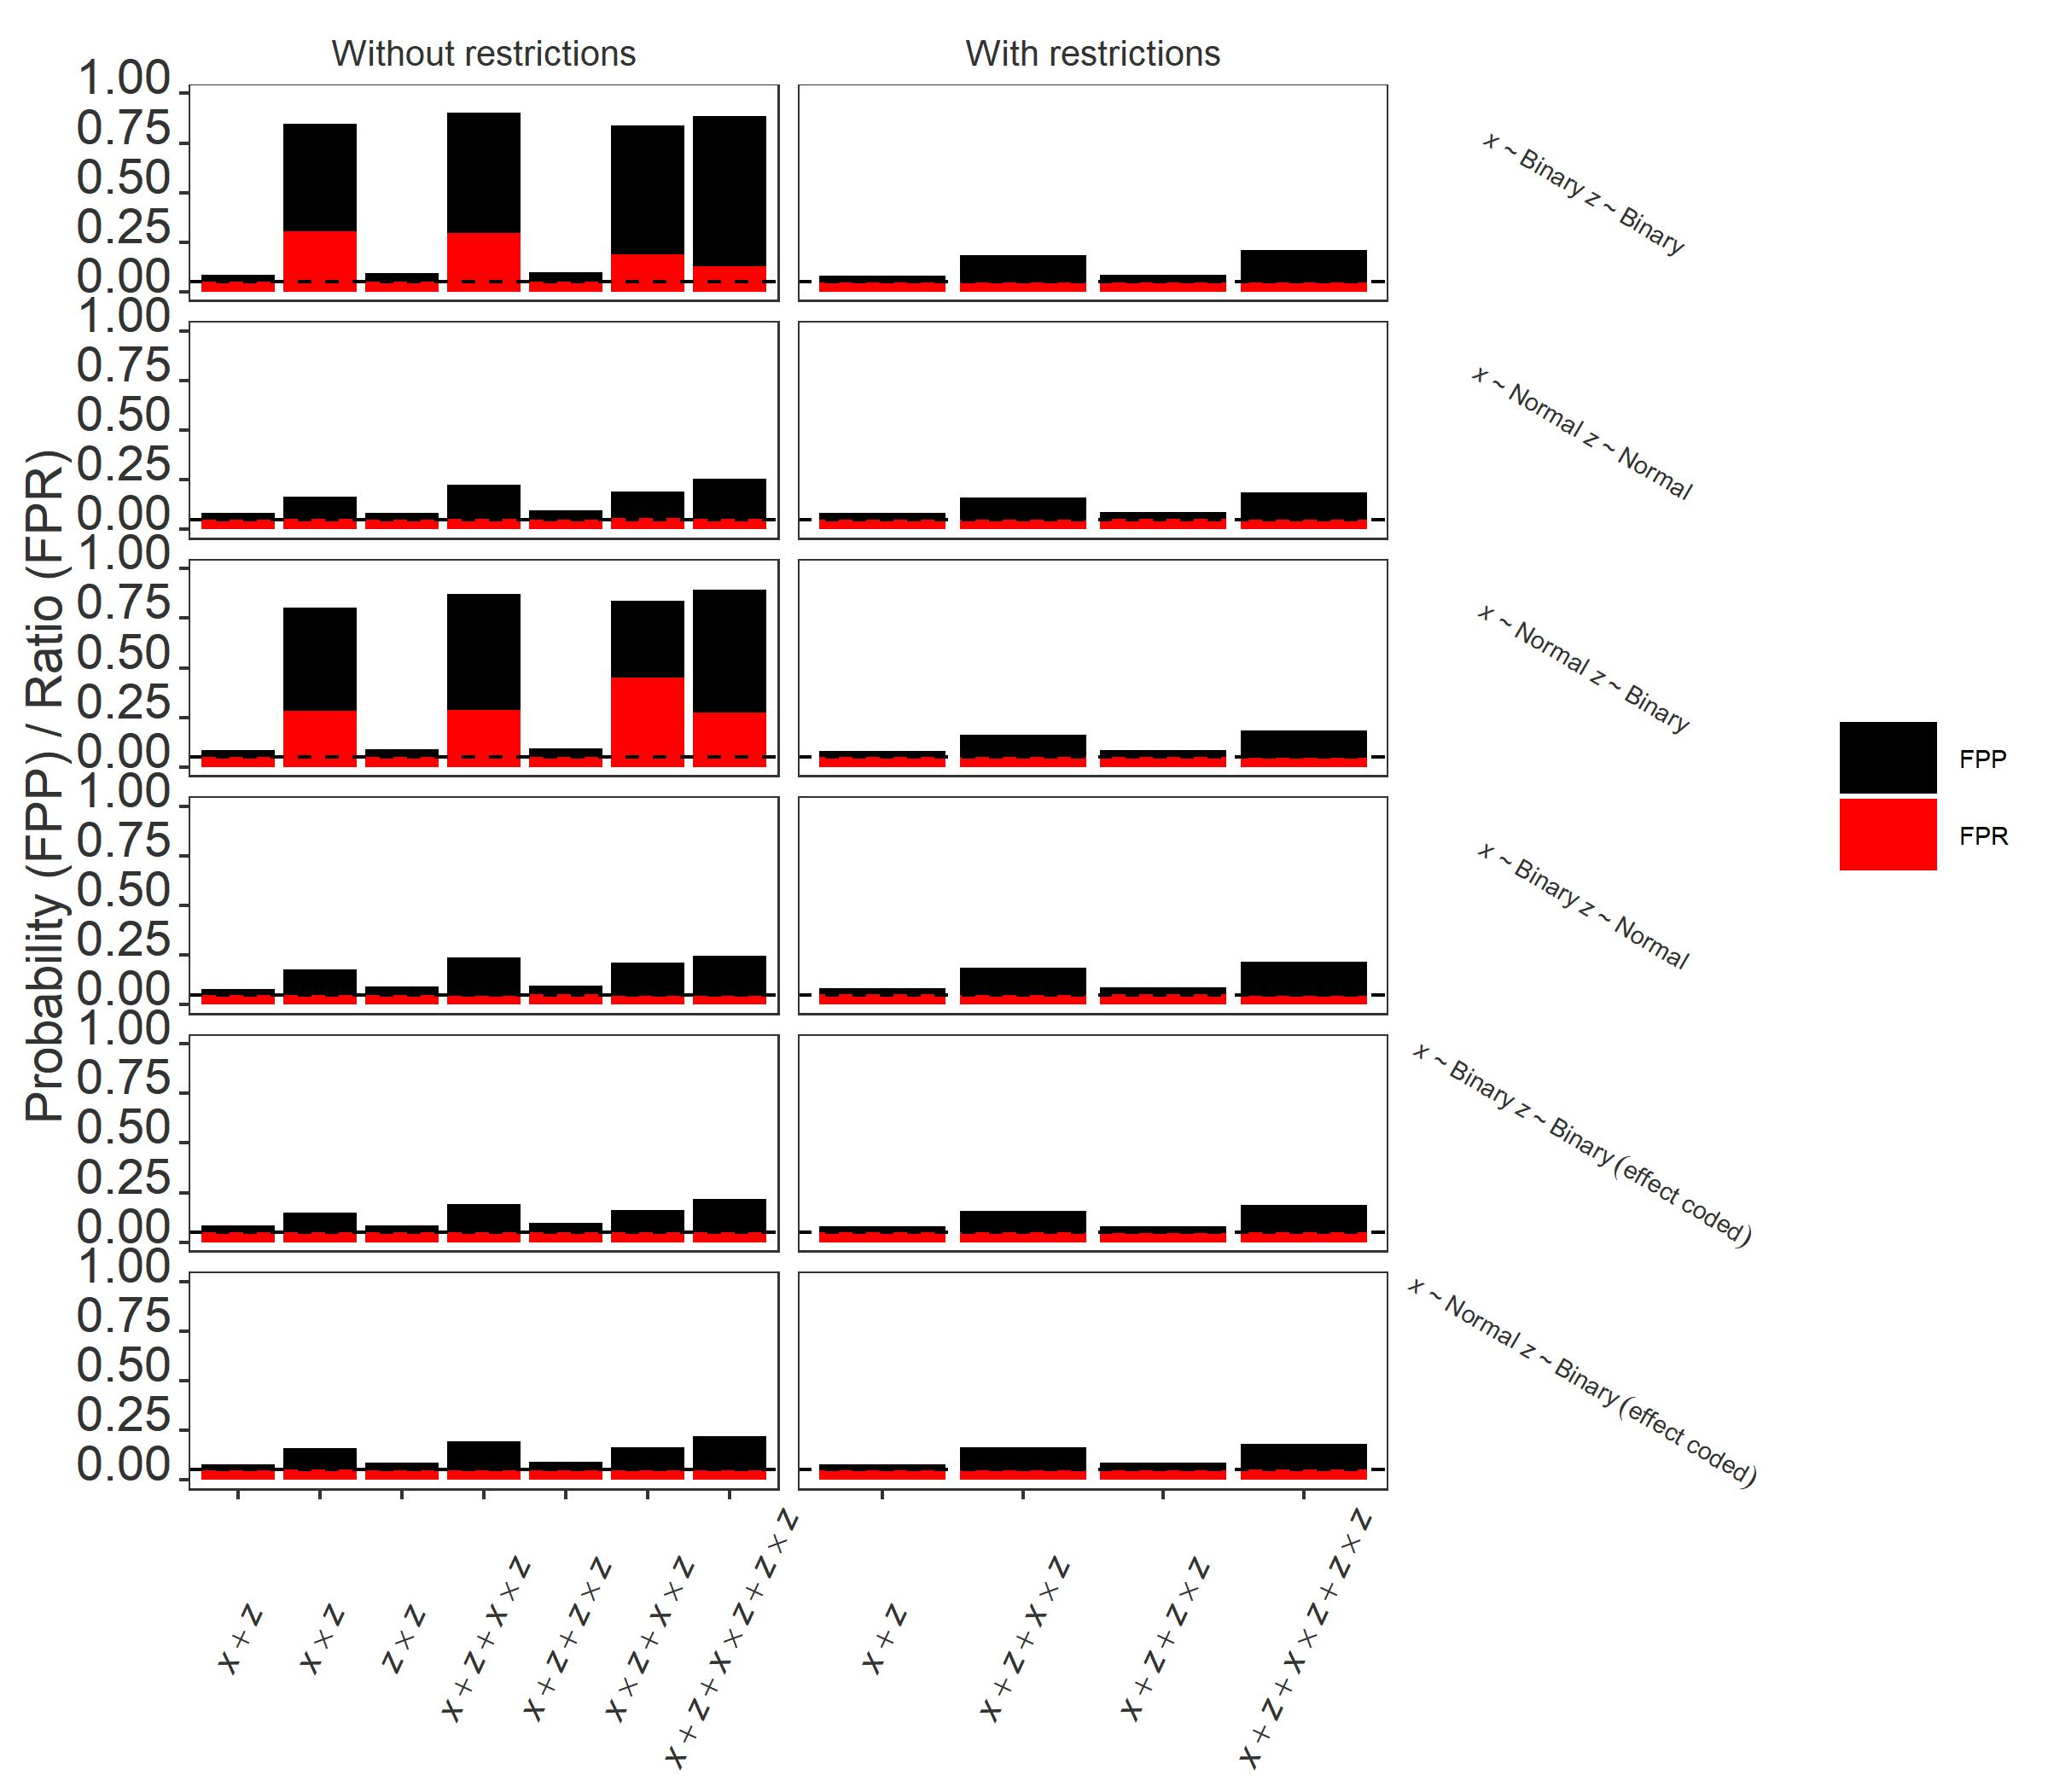
\includegraphics[width=1\textwidth]{R/Analysis/Result/Figures/Figure1CSIBon.jpeg}
\centering
\caption{False-positive probability and false-positive ratio when using three covariates instead of two as in the baseline model and when using Bonferroni correction. Black denotes the the false-positive probability and red denotes the false-positive ratio. Dashed blacked line shows the critical value, here set at 0.05. The description of the figure is otherwise the same as for Figure \ref{fig:appfigure7}.
}
\label{fig:appfigure11}
\end{figure}


\begin{landscape}
\begin{figure}[ht!]
%\figuretitle{Effect of increasing the sample size when using Bonferroni correction}
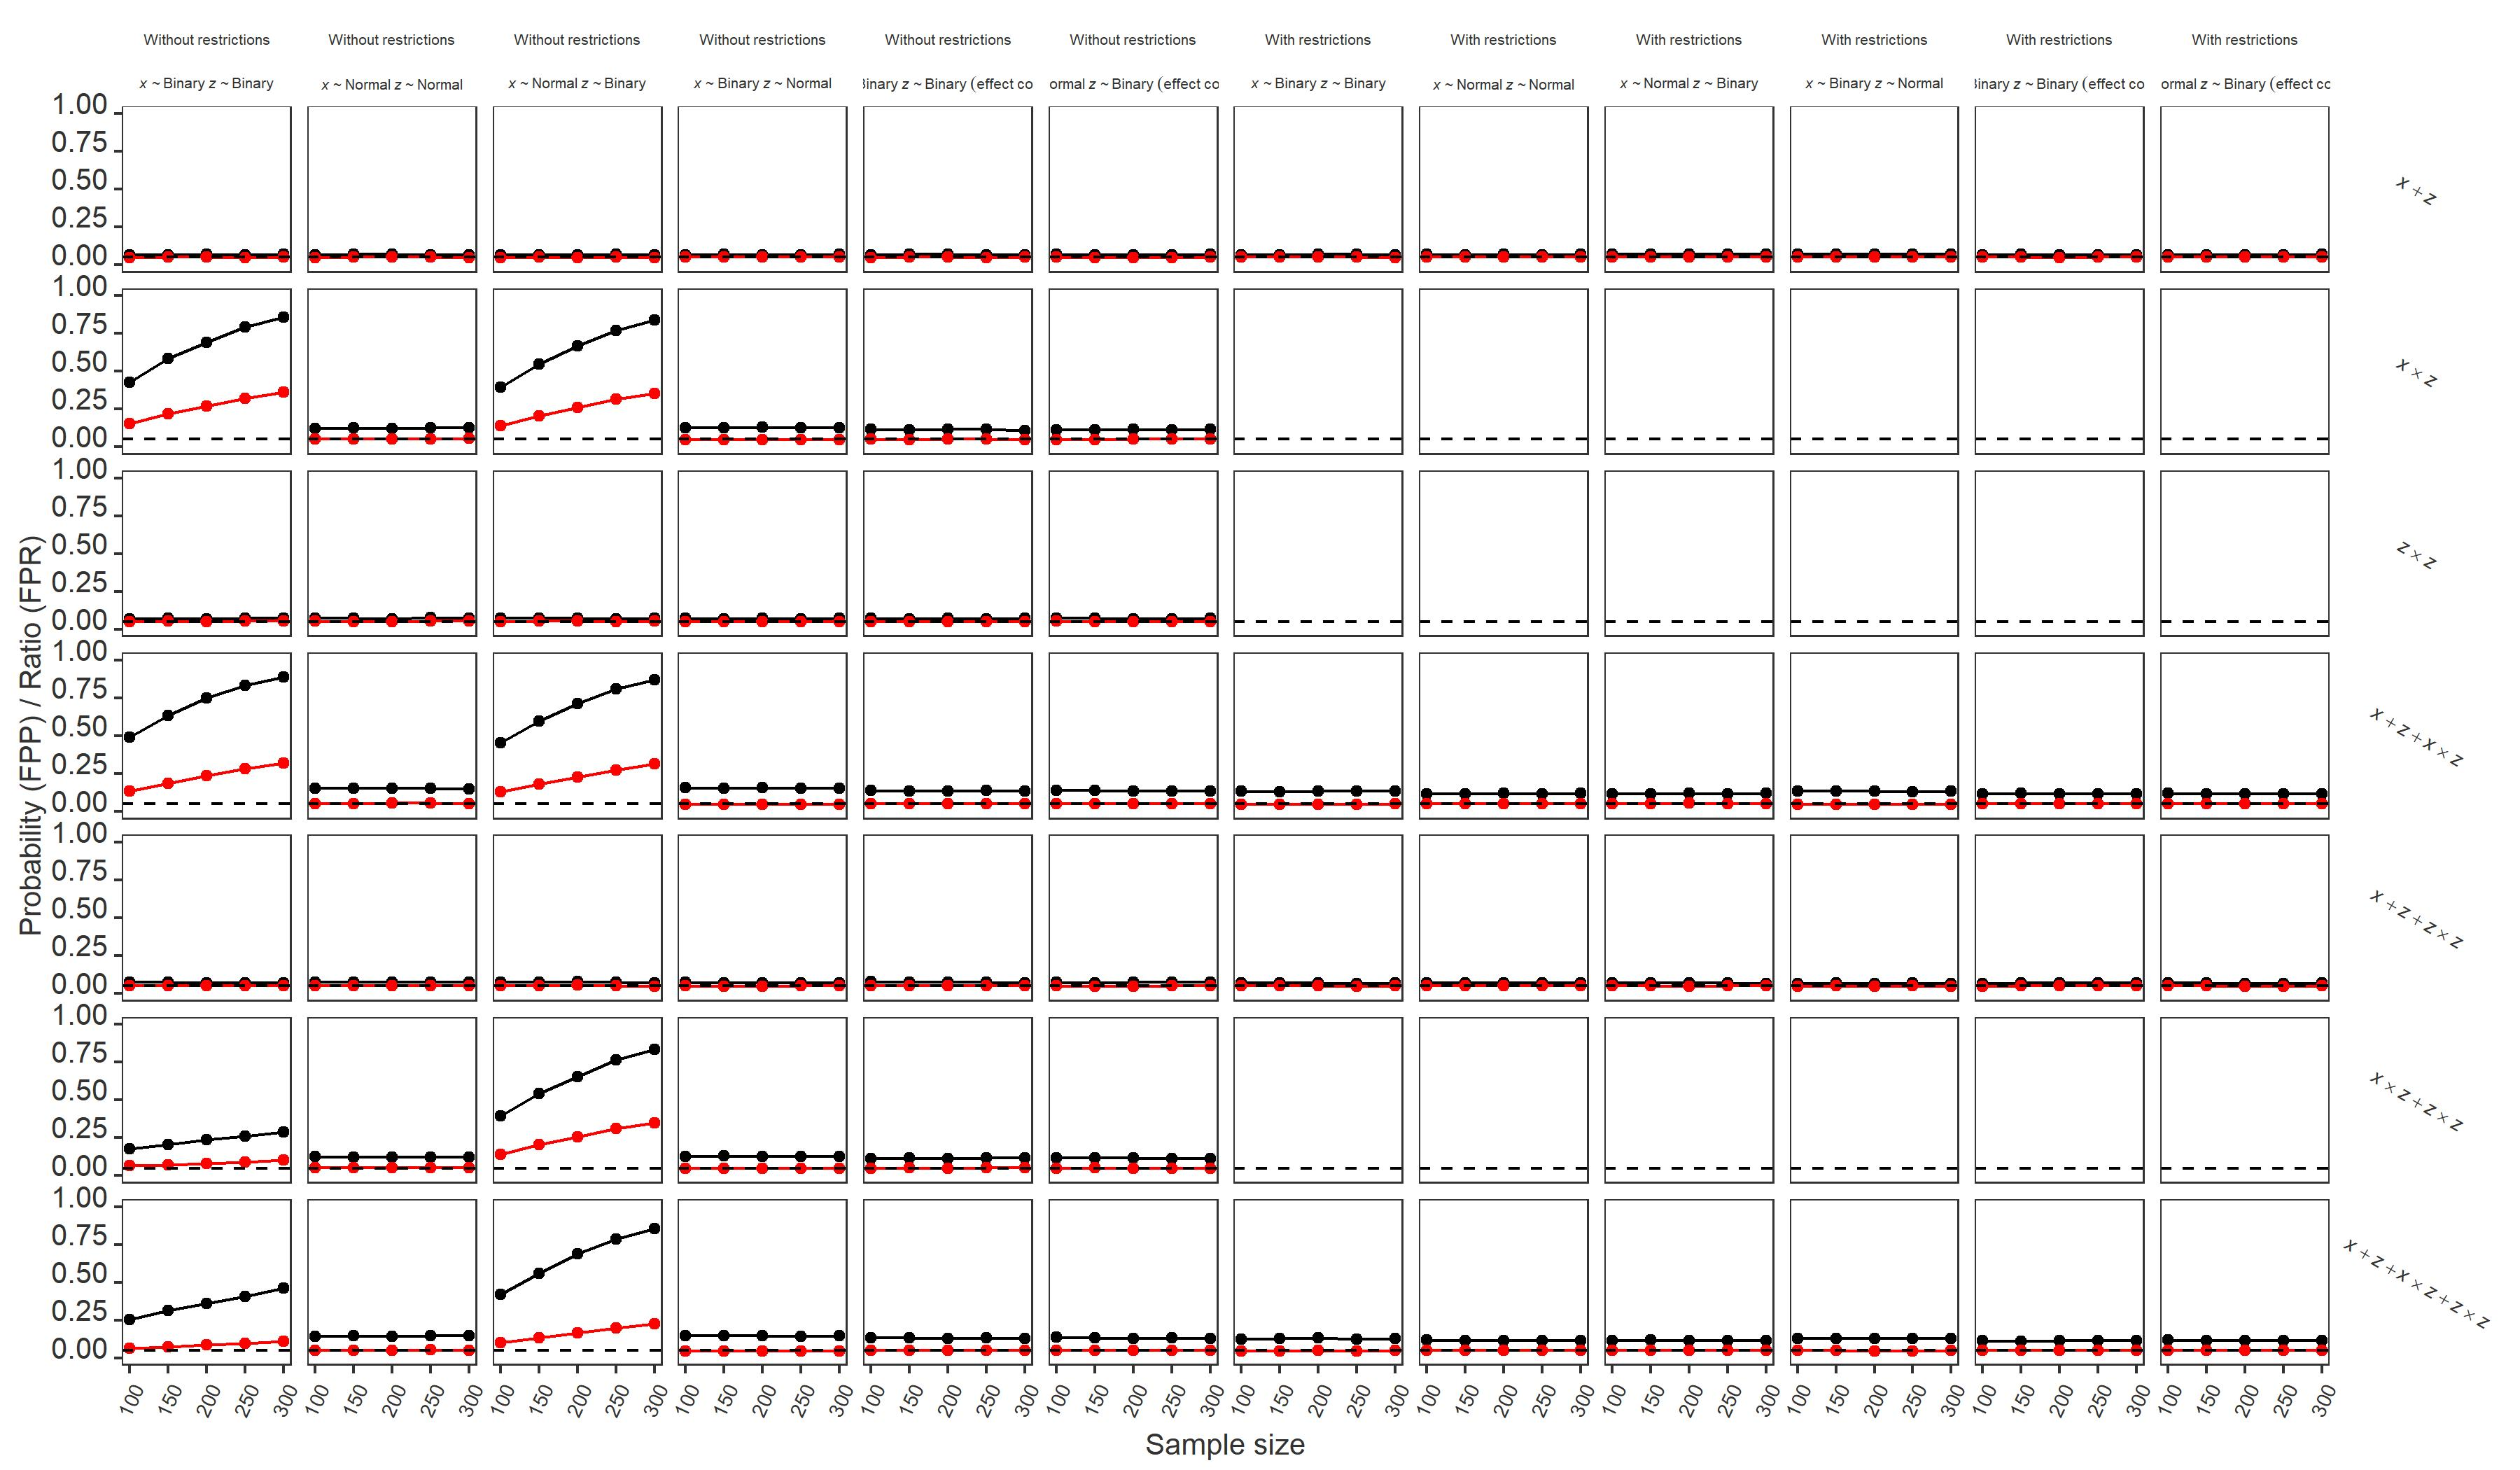
\includegraphics[scale=0.75]{R/Analysis/Result/Figures/Figure1DSIBon.jpeg}
\centering
\caption{Effect of increasing sample size for each model set and all combinations of data distributions (i.e., binary and normal) when using Bonferroni correction. Black denotes the false-positive probability and red denotes the false-positive ratio. Dashed blacked line shows the critical value, here set at 0.05. The description of the figure is otherwise the same as for Figure \ref{fig:appfigure1}.}
\label{fig:appfigure12}
\end{figure}
\end{landscape}

\subsection{Overview tables}
\label{overviewtable}
Readers interested in examining specific results from the simulation can consult the following overview tables. Table \ref{tab:apptabFull} and Table \ref{tab:apptabFullBC} contain the results for the full simulation of the different sets. Table \ref{tab:apptabFull} contains all the results when there is no correction of the p-value and \ref{tab:apptabFullBC} contains the results when Bonferroni correction is used. For each set, the result of the false-positive probability (FPP) and false-positive ratio (FPR) is shown with and without the restriction that main effects should always follow an interaction and for the different flexibilities used in the article i.e., increasing the number of covariates, increasing the number of dependent variables, and using several outlier criteria. This is shown using different data structures for the variable of interest and covariates. 
\begin{landscape}
\scriptsize
% latex table generated in R 4.0.5 by xtable 1.8-4 package
% Wed Aug 11 12:38:33 2021
\begin{longtable}{lccccccccc}
\caption{False-positive probability (FPP) and False-positive ratio (FPR) for the different model sets} \\ 
  \hline
Restrictions & Set & Type & Sample Size & Outlier exclusion & Correlation & Covariates & Dependent variables & FPP & FPR \\ 
  \hline
$Without$ & $\textit{x} + \textit{z}$ & $\textit{x} \sim Normal , \textit{z} \sim Normal$ & 200 & FALSE & 0.20 & 2.00 & 1.00 & 0.07 & 0.05 \\ 
  $Without$ & $\textit{x} + \textit{z}$ & $\textit{x} \sim Normal , \textit{z} \sim Normal$ & 200 & FALSE & 0.20 & 3.00 & 1.00 & 0.08 & 0.05 \\ 
  $Without$ & $\textit{x} + \textit{z}$ & $\textit{x} \sim Binary, \textit{z} \sim Binary$ & 200 & FALSE & 0.20 & 2.00 & 1.00 & 0.07 & 0.05 \\ 
  $Without$ & $\textit{x} + \textit{z}$ & $\textit{x} \sim Binary, \textit{z} \sim Binary$ & 200 & FALSE & 0.20 & 3.00 & 1.00 & 0.08 & 0.05 \\ 
  $Without$ & $\textit{x} + \textit{z}$ & $\textit{x} \sim Normal, \textit{z} \sim Binary$ & 200 & FALSE & 0.20 & 2.00 & 1.00 & 0.07 & 0.05 \\ 
  $Without$ & $\textit{x} + \textit{z}$ & $\textit{x} \sim Normal, \textit{z} \sim Binary$ & 200 & FALSE & 0.20 & 3.00 & 1.00 & 0.08 & 0.05 \\ 
  $Without$ & $\textit{x} + \textit{z}$ & $\textit{x} \sim Binary, \textit{z} \sim Normal$ & 200 & FALSE & 0.20 & 2.00 & 1.00 & 0.07 & 0.05 \\ 
  $Without$ & $\textit{x} + \textit{z}$ & $\textit{x} \sim Binary, \textit{z} \sim Normal$ & 200 & FALSE & 0.20 & 3.00 & 1.00 & 0.08 & 0.05 \\ 
  $Without$ & $\textit{x} + \textit{z}$ & $\textit{x} \sim Normal , \textit{z} \sim Normal$ &  50 & FALSE & 0.20 & 2.00 & 1.00 & 0.07 & 0.05 \\ 
  $Without$ & $\textit{x} + \textit{z}$ & $\textit{x} \sim Binary, \textit{z} \sim Binary$ &  50 & FALSE & 0.20 & 2.00 & 1.00 & 0.07 & 0.05 \\ 
  $Without$ & $\textit{x} + \textit{z}$ & $\textit{x} \sim Normal, \textit{z} \sim Binary$ &  50 & FALSE & 0.20 & 2.00 & 1.00 & 0.07 & 0.05 \\ 
  $Without$ & $\textit{x} + \textit{z}$ & $\textit{x} \sim Binary, \textit{z} \sim Normal$ &  50 & FALSE & 0.20 & 2.00 & 1.00 & 0.07 & 0.05 \\ 
  $Without$ & $\textit{x} + \textit{z}$ & $\textit{x} \sim Normal , \textit{z} \sim Normal$ & 100 & FALSE & 0.20 & 2.00 & 1.00 & 0.07 & 0.05 \\ 
  $Without$ & $\textit{x} + \textit{z}$ & $\textit{x} \sim Binary, \textit{z} \sim Binary$ & 100 & FALSE & 0.20 & 2.00 & 1.00 & 0.07 & 0.05 \\ 
  $Without$ & $\textit{x} + \textit{z}$ & $\textit{x} \sim Normal, \textit{z} \sim Binary$ & 100 & FALSE & 0.20 & 2.00 & 1.00 & 0.07 & 0.05 \\ 
  $Without$ & $\textit{x} + \textit{z}$ & $\textit{x} \sim Binary, \textit{z} \sim Normal$ & 100 & FALSE & 0.20 & 2.00 & 1.00 & 0.07 & 0.05 \\ 
  $Without$ & $\textit{x} + \textit{z}$ & $\textit{x} \sim Normal , \textit{z} \sim Normal$ & 150 & FALSE & 0.20 & 2.00 & 1.00 & 0.07 & 0.05 \\ 
  $Without$ & $\textit{x} + \textit{z}$ & $\textit{x} \sim Binary, \textit{z} \sim Binary$ & 150 & FALSE & 0.20 & 2.00 & 1.00 & 0.07 & 0.05 \\ 
  $Without$ & $\textit{x} + \textit{z}$ & $\textit{x} \sim Normal, \textit{z} \sim Binary$ & 150 & FALSE & 0.20 & 2.00 & 1.00 & 0.07 & 0.05 \\ 
  $Without$ & $\textit{x} + \textit{z}$ & $\textit{x} \sim Binary, \textit{z} \sim Normal$ & 150 & FALSE & 0.20 & 2.00 & 1.00 & 0.07 & 0.05 \\ 
  $Without$ & $\textit{x} + \textit{z}$ & $\textit{x} \sim Normal , \textit{z} \sim Normal$ & 250 & FALSE & 0.20 & 2.00 & 1.00 & 0.07 & 0.05 \\ 
  $Without$ & $\textit{x} + \textit{z}$ & $\textit{x} \sim Binary, \textit{z} \sim Binary$ & 250 & FALSE & 0.20 & 2.00 & 1.00 & 0.06 & 0.05 \\ 
  $Without$ & $\textit{x} + \textit{z}$ & $\textit{x} \sim Normal, \textit{z} \sim Binary$ & 250 & FALSE & 0.20 & 2.00 & 1.00 & 0.07 & 0.05 \\ 
  $Without$ & $\textit{x} + \textit{z}$ & $\textit{x} \sim Binary, \textit{z} \sim Normal$ & 250 & FALSE & 0.20 & 2.00 & 1.00 & 0.07 & 0.05 \\ 
  $Without$ & $\textit{x} + \textit{z}$ & $\textit{x} \sim Normal , \textit{z} \sim Normal$ & 300 & FALSE & 0.20 & 2.00 & 1.00 & 0.07 & 0.05 \\ 
  $Without$ & $\textit{x} + \textit{z}$ & $\textit{x} \sim Binary, \textit{z} \sim Binary$ & 300 & FALSE & 0.20 & 2.00 & 1.00 & 0.07 & 0.05 \\ 
  $Without$ & $\textit{x} + \textit{z}$ & $\textit{x} \sim Normal, \textit{z} \sim Binary$ & 300 & FALSE & 0.20 & 2.00 & 1.00 & 0.07 & 0.05 \\ 
  $Without$ & $\textit{x} + \textit{z}$ & $\textit{x} \sim Binary, \textit{z} \sim Normal$ & 300 & FALSE & 0.20 & 2.00 & 1.00 & 0.06 & 0.05 \\ 
  $Without$ & $\textit{x} + \textit{z}$ & $\textit{x} \sim Normal , \textit{z} \sim Normal$ & 200 & FALSE & 0.30 & 2.00 & 1.00 & 0.07 & 0.05 \\ 
  $Without$ & $\textit{x} + \textit{z}$ & $\textit{x} \sim Binary, \textit{z} \sim Binary$ & 200 & FALSE & 0.30 & 2.00 & 1.00 & 0.07 & 0.05 \\ 
  $Without$ & $\textit{x} + \textit{z}$ & $\textit{x} \sim Normal, \textit{z} \sim Binary$ & 200 & FALSE & 0.30 & 2.00 & 1.00 & 0.07 & 0.05 \\ 
  $Without$ & $\textit{x} + \textit{z}$ & $\textit{x} \sim Binary, \textit{z} \sim Normal$ & 200 & FALSE & 0.30 & 2.00 & 1.00 & 0.08 & 0.05 \\ 
  $Without$ & $\textit{x} + \textit{z}$ & $\textit{x} \sim Normal , \textit{z} \sim Normal$ & 200 & FALSE & 0.40 & 2.00 & 1.00 & 0.09 & 0.05 \\ 
  $Without$ & $\textit{x} + \textit{z}$ & $\textit{x} \sim Binary, \textit{z} \sim Binary$ & 200 & FALSE & 0.40 & 2.00 & 1.00 & 0.09 & 0.05 \\ 
  $Without$ & $\textit{x} + \textit{z}$ & $\textit{x} \sim Normal, \textit{z} \sim Binary$ & 200 & FALSE & 0.40 & 2.00 & 1.00 & 0.09 & 0.05 \\ 
  $Without$ & $\textit{x} + \textit{z}$ & $\textit{x} \sim Binary, \textit{z} \sim Normal$ & 200 & FALSE & 0.40 & 2.00 & 1.00 & 0.09 & 0.05 \\ 
  $Without$ & $\textit{x} + \textit{z}$ & $\textit{x} \sim Normal , \textit{z} \sim Normal$ & 200 & TRUE & 0.20 & 2.00 & 1.00 & 0.13 & 0.05 \\ 
  $Without$ & $\textit{x} + \textit{z}$ & $\textit{x} \sim Binary, \textit{z} \sim Binary$ & 200 & TRUE & 0.20 & 2.00 & 1.00 & 0.11 & 0.05 \\ 
  $Without$ & $\textit{x} + \textit{z}$ & $\textit{x} \sim Normal, \textit{z} \sim Binary$ & 200 & TRUE & 0.20 & 2.00 & 1.00 & 0.12 & 0.05 \\ 
  $Without$ & $\textit{x} + \textit{z}$ & $\textit{x} \sim Binary, \textit{z} \sim Normal$ & 200 & TRUE & 0.20 & 2.00 & 1.00 & 0.12 & 0.05 \\ 
  $Without$ & $\textit{x} + \textit{z}$ & $\textit{x} \sim Normal , \textit{z} \sim Normal$ & 200 & FALSE & 0.20 & 2.00 & 3.00 & 0.06 & 0.05 \\ 
  $Without$ & $\textit{x} + \textit{z}$ & $\textit{x} \sim Normal , \textit{z} \sim Normal$ & 200 & FALSE & 0.20 & 3.00 & 3.00 & 0.08 & 0.05 \\ 
  $Without$ & $\textit{x} + \textit{z}$ & $\textit{x} \sim Binary, \textit{z} \sim Binary$ & 200 & FALSE & 0.20 & 2.00 & 3.00 & 0.07 & 0.05 \\ 
  $Without$ & $\textit{x} + \textit{z}$ & $\textit{x} \sim Binary, \textit{z} \sim Binary$ & 200 & FALSE & 0.20 & 3.00 & 3.00 & 0.08 & 0.05 \\ 
  $Without$ & $\textit{x} + \textit{z}$ & $\textit{x} \sim Normal, \textit{z} \sim Binary$ & 200 & FALSE & 0.20 & 2.00 & 3.00 & 0.07 & 0.05 \\ 
  $Without$ & $\textit{x} + \textit{z}$ & $\textit{x} \sim Normal, \textit{z} \sim Binary$ & 200 & FALSE & 0.20 & 3.00 & 3.00 & 0.08 & 0.05 \\ 
  $Without$ & $\textit{x} + \textit{z}$ & $\textit{x} \sim Binary, \textit{z} \sim Normal$ & 200 & FALSE & 0.20 & 2.00 & 3.00 & 0.07 & 0.05 \\ 
  $Without$ & $\textit{x} + \textit{z}$ & $\textit{x} \sim Binary, \textit{z} \sim Normal$ & 200 & FALSE & 0.20 & 3.00 & 3.00 & 0.08 & 0.05 \\ 
  $Without$ & $\textit{x} \times \textit{z}$ & $\textit{x} \sim Normal , \textit{z} \sim Normal$ & 200 & FALSE & 0.20 & 2.00 & 1.00 & 0.17 & 0.12 \\ 
  $Without$ & $\textit{x} \times \textit{z}$ & $\textit{x} \sim Normal , \textit{z} \sim Normal$ & 200 & FALSE & 0.20 & 3.00 & 1.00 & 0.24 & 0.14 \\ 
  $Without$ & $\textit{x} \times \textit{z}$ & $\textit{x} \sim Binary, \textit{z} \sim Binary$ & 200 & FALSE & 0.20 & 2.00 & 1.00 & 0.82 & 0.64 \\ 
  $Without$ & $\textit{x} \times \textit{z}$ & $\textit{x} \sim Binary, \textit{z} \sim Binary$ & 200 & FALSE & 0.20 & 3.00 & 1.00 & 0.94 & 0.72 \\ 
  $Without$ & $\textit{x} \times \textit{z}$ & $\textit{x} \sim Normal, \textit{z} \sim Binary$ & 200 & FALSE & 0.20 & 2.00 & 1.00 & 0.79 & 0.62 \\ 
  $Without$ & $\textit{x} \times \textit{z}$ & $\textit{x} \sim Normal, \textit{z} \sim Binary$ & 200 & FALSE & 0.20 & 3.00 & 1.00 & 0.91 & 0.69 \\ 
  $Without$ & $\textit{x} \times \textit{z}$ & $\textit{x} \sim Binary, \textit{z} \sim Normal$ & 200 & FALSE & 0.20 & 2.00 & 1.00 & 0.17 & 0.10 \\ 
  $Without$ & $\textit{x} \times \textit{z}$ & $\textit{x} \sim Binary, \textit{z} \sim Normal$ & 200 & FALSE & 0.20 & 3.00 & 1.00 & 0.25 & 0.12 \\ 
  $Without$ & $\textit{x} \times \textit{z}$ & $\textit{x} \sim Normal , \textit{z} \sim Normal$ &  50 & FALSE & 0.20 & 2.00 & 1.00 & 0.18 & 0.12 \\ 
  $Without$ & $\textit{x} \times \textit{z}$ & $\textit{x} \sim Binary, \textit{z} \sim Binary$ &  50 & FALSE & 0.20 & 2.00 & 1.00 & 0.38 & 0.25 \\ 
  $Without$ & $\textit{x} \times \textit{z}$ & $\textit{x} \sim Normal, \textit{z} \sim Binary$ &  50 & FALSE & 0.20 & 2.00 & 1.00 & 0.35 & 0.24 \\ 
  $Without$ & $\textit{x} \times \textit{z}$ & $\textit{x} \sim Binary, \textit{z} \sim Normal$ &  50 & FALSE & 0.20 & 2.00 & 1.00 & 0.17 & 0.09 \\ 
  $Without$ & $\textit{x} \times \textit{z}$ & $\textit{x} \sim Normal , \textit{z} \sim Normal$ & 100 & FALSE & 0.20 & 2.00 & 1.00 & 0.17 & 0.12 \\ 
  $Without$ & $\textit{x} \times \textit{z}$ & $\textit{x} \sim Binary, \textit{z} \sim Binary$ & 100 & FALSE & 0.20 & 2.00 & 1.00 & 0.58 & 0.40 \\ 
  $Without$ & $\textit{x} \times \textit{z}$ & $\textit{x} \sim Normal, \textit{z} \sim Binary$ & 100 & FALSE & 0.20 & 2.00 & 1.00 & 0.54 & 0.38 \\ 
  $Without$ & $\textit{x} \times \textit{z}$ & $\textit{x} \sim Binary, \textit{z} \sim Normal$ & 100 & FALSE & 0.20 & 2.00 & 1.00 & 0.17 & 0.10 \\ 
  $Without$ & $\textit{x} \times \textit{z}$ & $\textit{x} \sim Normal , \textit{z} \sim Normal$ & 150 & FALSE & 0.20 & 2.00 & 1.00 & 0.18 & 0.13 \\ 
  $Without$ & $\textit{x} \times \textit{z}$ & $\textit{x} \sim Binary, \textit{z} \sim Binary$ & 150 & FALSE & 0.20 & 2.00 & 1.00 & 0.71 & 0.53 \\ 
  $Without$ & $\textit{x} \times \textit{z}$ & $\textit{x} \sim Normal, \textit{z} \sim Binary$ & 150 & FALSE & 0.20 & 2.00 & 1.00 & 0.69 & 0.51 \\ 
  $Without$ & $\textit{x} \times \textit{z}$ & $\textit{x} \sim Binary, \textit{z} \sim Normal$ & 150 & FALSE & 0.20 & 2.00 & 1.00 & 0.17 & 0.10 \\ 
  $Without$ & $\textit{x} \times \textit{z}$ & $\textit{x} \sim Normal , \textit{z} \sim Normal$ & 250 & FALSE & 0.20 & 2.00 & 1.00 & 0.17 & 0.12 \\ 
  $Without$ & $\textit{x} \times \textit{z}$ & $\textit{x} \sim Binary, \textit{z} \sim Binary$ & 250 & FALSE & 0.20 & 2.00 & 1.00 & 0.89 & 0.72 \\ 
  $Without$ & $\textit{x} \times \textit{z}$ & $\textit{x} \sim Normal, \textit{z} \sim Binary$ & 250 & FALSE & 0.20 & 2.00 & 1.00 & 0.87 & 0.70 \\ 
  $Without$ & $\textit{x} \times \textit{z}$ & $\textit{x} \sim Binary, \textit{z} \sim Normal$ & 250 & FALSE & 0.20 & 2.00 & 1.00 & 0.17 & 0.10 \\ 
  $Without$ & $\textit{x} \times \textit{z}$ & $\textit{x} \sim Normal , \textit{z} \sim Normal$ & 300 & FALSE & 0.20 & 2.00 & 1.00 & 0.17 & 0.12 \\ 
  $Without$ & $\textit{x} \times \textit{z}$ & $\textit{x} \sim Binary, \textit{z} \sim Binary$ & 300 & FALSE & 0.20 & 2.00 & 1.00 & 0.93 & 0.79 \\ 
  $Without$ & $\textit{x} \times \textit{z}$ & $\textit{x} \sim Normal, \textit{z} \sim Binary$ & 300 & FALSE & 0.20 & 2.00 & 1.00 & 0.92 & 0.77 \\ 
  $Without$ & $\textit{x} \times \textit{z}$ & $\textit{x} \sim Binary, \textit{z} \sim Normal$ & 300 & FALSE & 0.20 & 2.00 & 1.00 & 0.17 & 0.10 \\ 
  $Without$ & $\textit{x} \times \textit{z}$ & $\textit{x} \sim Normal , \textit{z} \sim Normal$ & 200 & FALSE & 0.30 & 2.00 & 1.00 & 0.19 & 0.14 \\ 
  $Without$ & $\textit{x} \times \textit{z}$ & $\textit{x} \sim Binary, \textit{z} \sim Binary$ & 200 & FALSE & 0.30 & 2.00 & 1.00 & 0.99 & 0.91 \\ 
  $Without$ & $\textit{x} \times \textit{z}$ & $\textit{x} \sim Normal, \textit{z} \sim Binary$ & 200 & FALSE & 0.30 & 2.00 & 1.00 & 0.98 & 0.90 \\ 
  $Without$ & $\textit{x} \times \textit{z}$ & $\textit{x} \sim Binary, \textit{z} \sim Normal$ & 200 & FALSE & 0.30 & 2.00 & 1.00 & 0.17 & 0.10 \\ 
  $Without$ & $\textit{x} \times \textit{z}$ & $\textit{x} \sim Normal , \textit{z} \sim Normal$ & 200 & FALSE & 0.40 & 2.00 & 1.00 & 0.22 & 0.15 \\ 
  $Without$ & $\textit{x} \times \textit{z}$ & $\textit{x} \sim Binary, \textit{z} \sim Binary$ & 200 & FALSE & 0.40 & 2.00 & 1.00 & 1.00 & 0.99 \\ 
  $Without$ & $\textit{x} \times \textit{z}$ & $\textit{x} \sim Normal, \textit{z} \sim Binary$ & 200 & FALSE & 0.40 & 2.00 & 1.00 & 1.00 & 0.99 \\ 
  $Without$ & $\textit{x} \times \textit{z}$ & $\textit{x} \sim Binary, \textit{z} \sim Normal$ & 200 & FALSE & 0.40 & 2.00 & 1.00 & 0.17 & 0.10 \\ 
  $Without$ & $\textit{x} \times \textit{z}$ & $\textit{x} \sim Normal , \textit{z} \sim Normal$ & 200 & TRUE & 0.20 & 2.00 & 1.00 & 0.34 & 0.12 \\ 
  $Without$ & $\textit{x} \times \textit{z}$ & $\textit{x} \sim Binary, \textit{z} \sim Binary$ & 200 & TRUE & 0.20 & 2.00 & 1.00 & 0.87 & 0.61 \\ 
  $Without$ & $\textit{x} \times \textit{z}$ & $\textit{x} \sim Normal, \textit{z} \sim Binary$ & 200 & TRUE & 0.20 & 2.00 & 1.00 & 0.86 & 0.55 \\ 
  $Without$ & $\textit{x} \times \textit{z}$ & $\textit{x} \sim Binary, \textit{z} \sim Normal$ & 200 & TRUE & 0.20 & 2.00 & 1.00 & 0.31 & 0.10 \\ 
  $Without$ & $\textit{x} \times \textit{z}$ & $\textit{x} \sim Normal , \textit{z} \sim Normal$ & 200 & FALSE & 0.20 & 2.00 & 3.00 & 0.17 & 0.12 \\ 
  $Without$ & $\textit{x} \times \textit{z}$ & $\textit{x} \sim Normal , \textit{z} \sim Normal$ & 200 & FALSE & 0.20 & 3.00 & 3.00 & 0.24 & 0.14 \\ 
  $Without$ & $\textit{x} \times \textit{z}$ & $\textit{x} \sim Binary, \textit{z} \sim Binary$ & 200 & FALSE & 0.20 & 2.00 & 3.00 & 0.82 & 0.64 \\ 
  $Without$ & $\textit{x} \times \textit{z}$ & $\textit{x} \sim Binary, \textit{z} \sim Binary$ & 200 & FALSE & 0.20 & 3.00 & 3.00 & 0.94 & 0.72 \\ 
  $Without$ & $\textit{x} \times \textit{z}$ & $\textit{x} \sim Normal, \textit{z} \sim Binary$ & 200 & FALSE & 0.20 & 2.00 & 3.00 & 0.79 & 0.62 \\ 
  $Without$ & $\textit{x} \times \textit{z}$ & $\textit{x} \sim Normal, \textit{z} \sim Binary$ & 200 & FALSE & 0.20 & 3.00 & 3.00 & 0.91 & 0.69 \\ 
  $Without$ & $\textit{x} \times \textit{z}$ & $\textit{x} \sim Binary, \textit{z} \sim Normal$ & 200 & FALSE & 0.20 & 2.00 & 3.00 & 0.17 & 0.10 \\ 
  $Without$ & $\textit{x} \times \textit{z}$ & $\textit{x} \sim Binary, \textit{z} \sim Normal$ & 200 & FALSE & 0.20 & 3.00 & 3.00 & 0.25 & 0.12 \\ 
  $Without$ & $\textit{z} \times \textit{z}$ & $\textit{x} \sim Normal , \textit{z} \sim Normal$ & 200 & FALSE & 0.20 & 2.00 & 1.00 & 0.05 & 0.05 \\ 
  $Without$ & $\textit{z} \times \textit{z}$ & $\textit{x} \sim Normal , \textit{z} \sim Normal$ & 200 & FALSE & 0.20 & 3.00 & 1.00 & 0.06 & 0.05 \\ 
  $Without$ & $\textit{z} \times \textit{z}$ & $\textit{x} \sim Binary, \textit{z} \sim Binary$ & 200 & FALSE & 0.20 & 2.00 & 1.00 & 0.05 & 0.05 \\ 
  $Without$ & $\textit{z} \times \textit{z}$ & $\textit{x} \sim Binary, \textit{z} \sim Binary$ & 200 & FALSE & 0.20 & 3.00 & 1.00 & 0.07 & 0.05 \\ 
  $Without$ & $\textit{z} \times \textit{z}$ & $\textit{x} \sim Normal, \textit{z} \sim Binary$ & 200 & FALSE & 0.20 & 2.00 & 1.00 & 0.05 & 0.05 \\ 
  $Without$ & $\textit{z} \times \textit{z}$ & $\textit{x} \sim Normal, \textit{z} \sim Binary$ & 200 & FALSE & 0.20 & 3.00 & 1.00 & 0.06 & 0.05 \\ 
  $Without$ & $\textit{z} \times \textit{z}$ & $\textit{x} \sim Binary, \textit{z} \sim Normal$ & 200 & FALSE & 0.20 & 2.00 & 1.00 & 0.05 & 0.05 \\ 
  $Without$ & $\textit{z} \times \textit{z}$ & $\textit{x} \sim Binary, \textit{z} \sim Normal$ & 200 & FALSE & 0.20 & 3.00 & 1.00 & 0.07 & 0.05 \\ 
  $Without$ & $\textit{z} \times \textit{z}$ & $\textit{x} \sim Normal , \textit{z} \sim Normal$ &  50 & FALSE & 0.20 & 2.00 & 1.00 & 0.05 & 0.05 \\ 
  $Without$ & $\textit{z} \times \textit{z}$ & $\textit{x} \sim Binary, \textit{z} \sim Binary$ &  50 & FALSE & 0.20 & 2.00 & 1.00 & 0.05 & 0.05 \\ 
  $Without$ & $\textit{z} \times \textit{z}$ & $\textit{x} \sim Normal, \textit{z} \sim Binary$ &  50 & FALSE & 0.20 & 2.00 & 1.00 & 0.05 & 0.05 \\ 
  $Without$ & $\textit{z} \times \textit{z}$ & $\textit{x} \sim Binary, \textit{z} \sim Normal$ &  50 & FALSE & 0.20 & 2.00 & 1.00 & 0.05 & 0.05 \\ 
  $Without$ & $\textit{z} \times \textit{z}$ & $\textit{x} \sim Normal , \textit{z} \sim Normal$ & 100 & FALSE & 0.20 & 2.00 & 1.00 & 0.05 & 0.05 \\ 
  $Without$ & $\textit{z} \times \textit{z}$ & $\textit{x} \sim Binary, \textit{z} \sim Binary$ & 100 & FALSE & 0.20 & 2.00 & 1.00 & 0.05 & 0.05 \\ 
  $Without$ & $\textit{z} \times \textit{z}$ & $\textit{x} \sim Normal, \textit{z} \sim Binary$ & 100 & FALSE & 0.20 & 2.00 & 1.00 & 0.05 & 0.05 \\ 
  $Without$ & $\textit{z} \times \textit{z}$ & $\textit{x} \sim Binary, \textit{z} \sim Normal$ & 100 & FALSE & 0.20 & 2.00 & 1.00 & 0.05 & 0.05 \\ 
  $Without$ & $\textit{z} \times \textit{z}$ & $\textit{x} \sim Normal , \textit{z} \sim Normal$ & 150 & FALSE & 0.20 & 2.00 & 1.00 & 0.05 & 0.05 \\ 
  $Without$ & $\textit{z} \times \textit{z}$ & $\textit{x} \sim Binary, \textit{z} \sim Binary$ & 150 & FALSE & 0.20 & 2.00 & 1.00 & 0.05 & 0.05 \\ 
  $Without$ & $\textit{z} \times \textit{z}$ & $\textit{x} \sim Normal, \textit{z} \sim Binary$ & 150 & FALSE & 0.20 & 2.00 & 1.00 & 0.05 & 0.05 \\ 
  $Without$ & $\textit{z} \times \textit{z}$ & $\textit{x} \sim Binary, \textit{z} \sim Normal$ & 150 & FALSE & 0.20 & 2.00 & 1.00 & 0.05 & 0.05 \\ 
  $Without$ & $\textit{z} \times \textit{z}$ & $\textit{x} \sim Normal , \textit{z} \sim Normal$ & 250 & FALSE & 0.20 & 2.00 & 1.00 & 0.05 & 0.05 \\ 
  $Without$ & $\textit{z} \times \textit{z}$ & $\textit{x} \sim Binary, \textit{z} \sim Binary$ & 250 & FALSE & 0.20 & 2.00 & 1.00 & 0.05 & 0.05 \\ 
  $Without$ & $\textit{z} \times \textit{z}$ & $\textit{x} \sim Normal, \textit{z} \sim Binary$ & 250 & FALSE & 0.20 & 2.00 & 1.00 & 0.05 & 0.05 \\ 
  $Without$ & $\textit{z} \times \textit{z}$ & $\textit{x} \sim Binary, \textit{z} \sim Normal$ & 250 & FALSE & 0.20 & 2.00 & 1.00 & 0.05 & 0.05 \\ 
  $Without$ & $\textit{z} \times \textit{z}$ & $\textit{x} \sim Normal , \textit{z} \sim Normal$ & 300 & FALSE & 0.20 & 2.00 & 1.00 & 0.05 & 0.05 \\ 
  $Without$ & $\textit{z} \times \textit{z}$ & $\textit{x} \sim Binary, \textit{z} \sim Binary$ & 300 & FALSE & 0.20 & 2.00 & 1.00 & 0.05 & 0.05 \\ 
  $Without$ & $\textit{z} \times \textit{z}$ & $\textit{x} \sim Normal, \textit{z} \sim Binary$ & 300 & FALSE & 0.20 & 2.00 & 1.00 & 0.05 & 0.05 \\ 
  $Without$ & $\textit{z} \times \textit{z}$ & $\textit{x} \sim Binary, \textit{z} \sim Normal$ & 300 & FALSE & 0.20 & 2.00 & 1.00 & 0.05 & 0.05 \\ 
  $Without$ & $\textit{z} \times \textit{z}$ & $\textit{x} \sim Normal , \textit{z} \sim Normal$ & 200 & FALSE & 0.30 & 2.00 & 1.00 & 0.05 & 0.05 \\ 
  $Without$ & $\textit{z} \times \textit{z}$ & $\textit{x} \sim Binary, \textit{z} \sim Binary$ & 200 & FALSE & 0.30 & 2.00 & 1.00 & 0.05 & 0.05 \\ 
  $Without$ & $\textit{z} \times \textit{z}$ & $\textit{x} \sim Normal, \textit{z} \sim Binary$ & 200 & FALSE & 0.30 & 2.00 & 1.00 & 0.05 & 0.05 \\ 
  $Without$ & $\textit{z} \times \textit{z}$ & $\textit{x} \sim Binary, \textit{z} \sim Normal$ & 200 & FALSE & 0.30 & 2.00 & 1.00 & 0.05 & 0.05 \\ 
  $Without$ & $\textit{z} \times \textit{z}$ & $\textit{x} \sim Normal , \textit{z} \sim Normal$ & 200 & FALSE & 0.40 & 2.00 & 1.00 & 0.05 & 0.05 \\ 
  $Without$ & $\textit{z} \times \textit{z}$ & $\textit{x} \sim Binary, \textit{z} \sim Binary$ & 200 & FALSE & 0.40 & 2.00 & 1.00 & 0.05 & 0.05 \\ 
  $Without$ & $\textit{z} \times \textit{z}$ & $\textit{x} \sim Normal, \textit{z} \sim Binary$ & 200 & FALSE & 0.40 & 2.00 & 1.00 & 0.05 & 0.05 \\ 
  $Without$ & $\textit{z} \times \textit{z}$ & $\textit{x} \sim Binary, \textit{z} \sim Normal$ & 200 & FALSE & 0.40 & 2.00 & 1.00 & 0.05 & 0.05 \\ 
  $Without$ & $\textit{z} \times \textit{z}$ & $\textit{x} \sim Normal , \textit{z} \sim Normal$ & 200 & TRUE & 0.20 & 2.00 & 1.00 & 0.11 & 0.05 \\ 
  $Without$ & $\textit{z} \times \textit{z}$ & $\textit{x} \sim Binary, \textit{z} \sim Binary$ & 200 & TRUE & 0.20 & 2.00 & 1.00 & 0.09 & 0.05 \\ 
  $Without$ & $\textit{z} \times \textit{z}$ & $\textit{x} \sim Normal, \textit{z} \sim Binary$ & 200 & TRUE & 0.20 & 2.00 & 1.00 & 0.09 & 0.05 \\ 
  $Without$ & $\textit{z} \times \textit{z}$ & $\textit{x} \sim Binary, \textit{z} \sim Normal$ & 200 & TRUE & 0.20 & 2.00 & 1.00 & 0.10 & 0.05 \\ 
  $Without$ & $\textit{z} \times \textit{z}$ & $\textit{x} \sim Normal , \textit{z} \sim Normal$ & 200 & FALSE & 0.20 & 2.00 & 3.00 & 0.05 & 0.05 \\ 
  $Without$ & $\textit{z} \times \textit{z}$ & $\textit{x} \sim Normal , \textit{z} \sim Normal$ & 200 & FALSE & 0.20 & 3.00 & 3.00 & 0.06 & 0.05 \\ 
  $Without$ & $\textit{z} \times \textit{z}$ & $\textit{x} \sim Binary, \textit{z} \sim Binary$ & 200 & FALSE & 0.20 & 2.00 & 3.00 & 0.05 & 0.05 \\ 
  $Without$ & $\textit{z} \times \textit{z}$ & $\textit{x} \sim Binary, \textit{z} \sim Binary$ & 200 & FALSE & 0.20 & 3.00 & 3.00 & 0.07 & 0.05 \\ 
  $Without$ & $\textit{z} \times \textit{z}$ & $\textit{x} \sim Normal, \textit{z} \sim Binary$ & 200 & FALSE & 0.20 & 2.00 & 3.00 & 0.05 & 0.05 \\ 
  $Without$ & $\textit{z} \times \textit{z}$ & $\textit{x} \sim Normal, \textit{z} \sim Binary$ & 200 & FALSE & 0.20 & 3.00 & 3.00 & 0.06 & 0.05 \\ 
  $Without$ & $\textit{z} \times \textit{z}$ & $\textit{x} \sim Binary, \textit{z} \sim Normal$ & 200 & FALSE & 0.20 & 2.00 & 3.00 & 0.05 & 0.05 \\ 
  $Without$ & $\textit{z} \times \textit{z}$ & $\textit{x} \sim Binary, \textit{z} \sim Normal$ & 200 & FALSE & 0.20 & 3.00 & 3.00 & 0.07 & 0.05 \\ 
  $Without$ & $\textit{x} + \textit{z} + \textit{x} \times \textit{z}$ & $\textit{x} \sim Normal , \textit{z} \sim Normal$ & 200 & FALSE & 0.20 & 2.00 & 1.00 & 0.23 & 0.12 \\ 
  $Without$ & $\textit{x} + \textit{z} + \textit{x} \times \textit{z}$ & $\textit{x} \sim Normal , \textit{z} \sim Normal$ & 200 & FALSE & 0.20 & 3.00 & 1.00 & 0.37 & 0.14 \\ 
  $Without$ & $\textit{x} + \textit{z} + \textit{x} \times \textit{z}$ & $\textit{x} \sim Binary, \textit{z} \sim Binary$ & 200 & FALSE & 0.20 & 2.00 & 1.00 & 0.86 & 0.39 \\ 
  $Without$ & $\textit{x} + \textit{z} + \textit{x} \times \textit{z}$ & $\textit{x} \sim Binary, \textit{z} \sim Binary$ & 200 & FALSE & 0.20 & 3.00 & 1.00 & 0.97 & 0.46 \\ 
  $Without$ & $\textit{x} + \textit{z} + \textit{x} \times \textit{z}$ & $\textit{x} \sim Normal, \textit{z} \sim Binary$ & 200 & FALSE & 0.20 & 2.00 & 1.00 & 0.83 & 0.39 \\ 
  $Without$ & $\textit{x} + \textit{z} + \textit{x} \times \textit{z}$ & $\textit{x} \sim Normal, \textit{z} \sim Binary$ & 200 & FALSE & 0.20 & 3.00 & 1.00 & 0.95 & 0.46 \\ 
  $Without$ & $\textit{x} + \textit{z} + \textit{x} \times \textit{z}$ & $\textit{x} \sim Binary, \textit{z} \sim Normal$ & 200 & FALSE & 0.20 & 2.00 & 1.00 & 0.23 & 0.10 \\ 
  $Without$ & $\textit{x} + \textit{z} + \textit{x} \times \textit{z}$ & $\textit{x} \sim Binary, \textit{z} \sim Normal$ & 200 & FALSE & 0.20 & 3.00 & 1.00 & 0.37 & 0.11 \\ 
  $Without$ & $\textit{x} + \textit{z} + \textit{x} \times \textit{z}$ & $\textit{x} \sim Normal , \textit{z} \sim Normal$ &  50 & FALSE & 0.20 & 2.00 & 1.00 & 0.24 & 0.11 \\ 
  $Without$ & $\textit{x} + \textit{z} + \textit{x} \times \textit{z}$ & $\textit{x} \sim Binary, \textit{z} \sim Binary$ &  50 & FALSE & 0.20 & 2.00 & 1.00 & 0.47 & 0.17 \\ 
  $Without$ & $\textit{x} + \textit{z} + \textit{x} \times \textit{z}$ & $\textit{x} \sim Normal, \textit{z} \sim Binary$ &  50 & FALSE & 0.20 & 2.00 & 1.00 & 0.44 & 0.18 \\ 
  $Without$ & $\textit{x} + \textit{z} + \textit{x} \times \textit{z}$ & $\textit{x} \sim Binary, \textit{z} \sim Normal$ &  50 & FALSE & 0.20 & 2.00 & 1.00 & 0.23 & 0.10 \\ 
  $Without$ & $\textit{x} + \textit{z} + \textit{x} \times \textit{z}$ & $\textit{x} \sim Normal , \textit{z} \sim Normal$ & 100 & FALSE & 0.20 & 2.00 & 1.00 & 0.24 & 0.11 \\ 
  $Without$ & $\textit{x} + \textit{z} + \textit{x} \times \textit{z}$ & $\textit{x} \sim Binary, \textit{z} \sim Binary$ & 100 & FALSE & 0.20 & 2.00 & 1.00 & 0.65 & 0.25 \\ 
  $Without$ & $\textit{x} + \textit{z} + \textit{x} \times \textit{z}$ & $\textit{x} \sim Normal, \textit{z} \sim Binary$ & 100 & FALSE & 0.20 & 2.00 & 1.00 & 0.60 & 0.25 \\ 
  $Without$ & $\textit{x} + \textit{z} + \textit{x} \times \textit{z}$ & $\textit{x} \sim Binary, \textit{z} \sim Normal$ & 100 & FALSE & 0.20 & 2.00 & 1.00 & 0.22 & 0.09 \\ 
  $Without$ & $\textit{x} + \textit{z} + \textit{x} \times \textit{z}$ & $\textit{x} \sim Normal , \textit{z} \sim Normal$ & 150 & FALSE & 0.20 & 2.00 & 1.00 & 0.24 & 0.12 \\ 
  $Without$ & $\textit{x} + \textit{z} + \textit{x} \times \textit{z}$ & $\textit{x} \sim Binary, \textit{z} \sim Binary$ & 150 & FALSE & 0.20 & 2.00 & 1.00 & 0.78 & 0.33 \\ 
  $Without$ & $\textit{x} + \textit{z} + \textit{x} \times \textit{z}$ & $\textit{x} \sim Normal, \textit{z} \sim Binary$ & 150 & FALSE & 0.20 & 2.00 & 1.00 & 0.73 & 0.32 \\ 
  $Without$ & $\textit{x} + \textit{z} + \textit{x} \times \textit{z}$ & $\textit{x} \sim Binary, \textit{z} \sim Normal$ & 150 & FALSE & 0.20 & 2.00 & 1.00 & 0.22 & 0.10 \\ 
  $Without$ & $\textit{x} + \textit{z} + \textit{x} \times \textit{z}$ & $\textit{x} \sim Normal , \textit{z} \sim Normal$ & 250 & FALSE & 0.20 & 2.00 & 1.00 & 0.24 & 0.12 \\ 
  $Without$ & $\textit{x} + \textit{z} + \textit{x} \times \textit{z}$ & $\textit{x} \sim Binary, \textit{z} \sim Binary$ & 250 & FALSE & 0.20 & 2.00 & 1.00 & 0.92 & 0.44 \\ 
  $Without$ & $\textit{x} + \textit{z} + \textit{x} \times \textit{z}$ & $\textit{x} \sim Normal, \textit{z} \sim Binary$ & 250 & FALSE & 0.20 & 2.00 & 1.00 & 0.90 & 0.44 \\ 
  $Without$ & $\textit{x} + \textit{z} + \textit{x} \times \textit{z}$ & $\textit{x} \sim Binary, \textit{z} \sim Normal$ & 250 & FALSE & 0.20 & 2.00 & 1.00 & 0.22 & 0.10 \\ 
  $Without$ & $\textit{x} + \textit{z} + \textit{x} \times \textit{z}$ & $\textit{x} \sim Normal , \textit{z} \sim Normal$ & 300 & FALSE & 0.20 & 2.00 & 1.00 & 0.23 & 0.12 \\ 
  $Without$ & $\textit{x} + \textit{z} + \textit{x} \times \textit{z}$ & $\textit{x} \sim Binary, \textit{z} \sim Binary$ & 300 & FALSE & 0.20 & 2.00 & 1.00 & 0.96 & 0.48 \\ 
  $Without$ & $\textit{x} + \textit{z} + \textit{x} \times \textit{z}$ & $\textit{x} \sim Normal, \textit{z} \sim Binary$ & 300 & FALSE & 0.20 & 2.00 & 1.00 & 0.94 & 0.48 \\ 
  $Without$ & $\textit{x} + \textit{z} + \textit{x} \times \textit{z}$ & $\textit{x} \sim Binary, \textit{z} \sim Normal$ & 300 & FALSE & 0.20 & 2.00 & 1.00 & 0.22 & 0.10 \\ 
  $Without$ & $\textit{x} + \textit{z} + \textit{x} \times \textit{z}$ & $\textit{x} \sim Normal , \textit{z} \sim Normal$ & 200 & FALSE & 0.30 & 2.00 & 1.00 & 0.28 & 0.12 \\ 
  $Without$ & $\textit{x} + \textit{z} + \textit{x} \times \textit{z}$ & $\textit{x} \sim Binary, \textit{z} \sim Binary$ & 200 & FALSE & 0.30 & 2.00 & 1.00 & 1.00 & 0.57 \\ 
  $Without$ & $\textit{x} + \textit{z} + \textit{x} \times \textit{z}$ & $\textit{x} \sim Normal, \textit{z} \sim Binary$ & 200 & FALSE & 0.30 & 2.00 & 1.00 & 0.99 & 0.57 \\ 
  $Without$ & $\textit{x} + \textit{z} + \textit{x} \times \textit{z}$ & $\textit{x} \sim Binary, \textit{z} \sim Normal$ & 200 & FALSE & 0.30 & 2.00 & 1.00 & 0.25 & 0.10 \\ 
  $Without$ & $\textit{x} + \textit{z} + \textit{x} \times \textit{z}$ & $\textit{x} \sim Normal , \textit{z} \sim Normal$ & 200 & FALSE & 0.40 & 2.00 & 1.00 & 0.35 & 0.13 \\ 
  $Without$ & $\textit{x} + \textit{z} + \textit{x} \times \textit{z}$ & $\textit{x} \sim Binary, \textit{z} \sim Binary$ & 200 & FALSE & 0.40 & 2.00 & 1.00 & 1.00 & 0.62 \\ 
  $Without$ & $\textit{x} + \textit{z} + \textit{x} \times \textit{z}$ & $\textit{x} \sim Normal, \textit{z} \sim Binary$ & 200 & FALSE & 0.40 & 2.00 & 1.00 & 1.00 & 0.62 \\ 
  $Without$ & $\textit{x} + \textit{z} + \textit{x} \times \textit{z}$ & $\textit{x} \sim Binary, \textit{z} \sim Normal$ & 200 & FALSE & 0.40 & 2.00 & 1.00 & 0.29 & 0.10 \\ 
  $Without$ & $\textit{x} + \textit{z} + \textit{x} \times \textit{z}$ & $\textit{x} \sim Normal , \textit{z} \sim Normal$ & 200 & TRUE & 0.20 & 2.00 & 1.00 & 0.41 & 0.11 \\ 
  $Without$ & $\textit{x} + \textit{z} + \textit{x} \times \textit{z}$ & $\textit{x} \sim Binary, \textit{z} \sim Binary$ & 200 & TRUE & 0.20 & 2.00 & 1.00 & 0.92 & 0.37 \\ 
  $Without$ & $\textit{x} + \textit{z} + \textit{x} \times \textit{z}$ & $\textit{x} \sim Normal, \textit{z} \sim Binary$ & 200 & TRUE & 0.20 & 2.00 & 1.00 & 0.90 & 0.35 \\ 
  $Without$ & $\textit{x} + \textit{z} + \textit{x} \times \textit{z}$ & $\textit{x} \sim Binary, \textit{z} \sim Normal$ & 200 & TRUE & 0.20 & 2.00 & 1.00 & 0.38 & 0.10 \\ 
  $Without$ & $\textit{x} + \textit{z} + \textit{x} \times \textit{z}$ & $\textit{x} \sim Normal , \textit{z} \sim Normal$ & 200 & FALSE & 0.20 & 2.00 & 3.00 & 0.23 & 0.12 \\ 
  $Without$ & $\textit{x} + \textit{z} + \textit{x} \times \textit{z}$ & $\textit{x} \sim Normal , \textit{z} \sim Normal$ & 200 & FALSE & 0.20 & 3.00 & 3.00 & 0.37 & 0.14 \\ 
  $Without$ & $\textit{x} + \textit{z} + \textit{x} \times \textit{z}$ & $\textit{x} \sim Binary, \textit{z} \sim Binary$ & 200 & FALSE & 0.20 & 2.00 & 3.00 & 0.87 & 0.39 \\ 
  $Without$ & $\textit{x} + \textit{z} + \textit{x} \times \textit{z}$ & $\textit{x} \sim Binary, \textit{z} \sim Binary$ & 200 & FALSE & 0.20 & 3.00 & 3.00 & 0.97 & 0.46 \\ 
  $Without$ & $\textit{x} + \textit{z} + \textit{x} \times \textit{z}$ & $\textit{x} \sim Normal, \textit{z} \sim Binary$ & 200 & FALSE & 0.20 & 2.00 & 3.00 & 0.83 & 0.39 \\ 
  $Without$ & $\textit{x} + \textit{z} + \textit{x} \times \textit{z}$ & $\textit{x} \sim Normal, \textit{z} \sim Binary$ & 200 & FALSE & 0.20 & 3.00 & 3.00 & 0.95 & 0.46 \\ 
  $Without$ & $\textit{x} + \textit{z} + \textit{x} \times \textit{z}$ & $\textit{x} \sim Binary, \textit{z} \sim Normal$ & 200 & FALSE & 0.20 & 2.00 & 3.00 & 0.23 & 0.10 \\ 
  $Without$ & $\textit{x} + \textit{z} + \textit{x} \times \textit{z}$ & $\textit{x} \sim Binary, \textit{z} \sim Normal$ & 200 & FALSE & 0.20 & 3.00 & 3.00 & 0.37 & 0.11 \\ 
  $Without$ & $\textit{x} + \textit{z} + \textit{z} \times \textit{z}$ & $\textit{x} \sim Normal , \textit{z} \sim Normal$ & 200 & FALSE & 0.20 & 2.00 & 1.00 & 0.07 & 0.05 \\ 
  $Without$ & $\textit{x} + \textit{z} + \textit{z} \times \textit{z}$ & $\textit{x} \sim Normal , \textit{z} \sim Normal$ & 200 & FALSE & 0.20 & 3.00 & 1.00 & 0.09 & 0.05 \\ 
  $Without$ & $\textit{x} + \textit{z} + \textit{z} \times \textit{z}$ & $\textit{x} \sim Binary, \textit{z} \sim Binary$ & 200 & FALSE & 0.20 & 2.00 & 1.00 & 0.06 & 0.05 \\ 
  $Without$ & $\textit{x} + \textit{z} + \textit{z} \times \textit{z}$ & $\textit{x} \sim Binary, \textit{z} \sim Binary$ & 200 & FALSE & 0.20 & 3.00 & 1.00 & 0.09 & 0.05 \\ 
  $Without$ & $\textit{x} + \textit{z} + \textit{z} \times \textit{z}$ & $\textit{x} \sim Normal, \textit{z} \sim Binary$ & 200 & FALSE & 0.20 & 2.00 & 1.00 & 0.07 & 0.05 \\ 
  $Without$ & $\textit{x} + \textit{z} + \textit{z} \times \textit{z}$ & $\textit{x} \sim Normal, \textit{z} \sim Binary$ & 200 & FALSE & 0.20 & 3.00 & 1.00 & 0.09 & 0.05 \\ 
  $Without$ & $\textit{x} + \textit{z} + \textit{z} \times \textit{z}$ & $\textit{x} \sim Binary, \textit{z} \sim Normal$ & 200 & FALSE & 0.20 & 2.00 & 1.00 & 0.06 & 0.05 \\ 
  $Without$ & $\textit{x} + \textit{z} + \textit{z} \times \textit{z}$ & $\textit{x} \sim Binary, \textit{z} \sim Normal$ & 200 & FALSE & 0.20 & 3.00 & 1.00 & 0.09 & 0.05 \\ 
  $Without$ & $\textit{x} + \textit{z} + \textit{z} \times \textit{z}$ & $\textit{x} \sim Normal , \textit{z} \sim Normal$ &  50 & FALSE & 0.20 & 2.00 & 1.00 & 0.07 & 0.05 \\ 
  $Without$ & $\textit{x} + \textit{z} + \textit{z} \times \textit{z}$ & $\textit{x} \sim Binary, \textit{z} \sim Binary$ &  50 & FALSE & 0.20 & 2.00 & 1.00 & 0.07 & 0.05 \\ 
  $Without$ & $\textit{x} + \textit{z} + \textit{z} \times \textit{z}$ & $\textit{x} \sim Normal, \textit{z} \sim Binary$ &  50 & FALSE & 0.20 & 2.00 & 1.00 & 0.07 & 0.05 \\ 
  $Without$ & $\textit{x} + \textit{z} + \textit{z} \times \textit{z}$ & $\textit{x} \sim Binary, \textit{z} \sim Normal$ &  50 & FALSE & 0.20 & 2.00 & 1.00 & 0.07 & 0.05 \\ 
  $Without$ & $\textit{x} + \textit{z} + \textit{z} \times \textit{z}$ & $\textit{x} \sim Normal , \textit{z} \sim Normal$ & 100 & FALSE & 0.20 & 2.00 & 1.00 & 0.07 & 0.05 \\ 
  $Without$ & $\textit{x} + \textit{z} + \textit{z} \times \textit{z}$ & $\textit{x} \sim Binary, \textit{z} \sim Binary$ & 100 & FALSE & 0.20 & 2.00 & 1.00 & 0.06 & 0.05 \\ 
  $Without$ & $\textit{x} + \textit{z} + \textit{z} \times \textit{z}$ & $\textit{x} \sim Normal, \textit{z} \sim Binary$ & 100 & FALSE & 0.20 & 2.00 & 1.00 & 0.07 & 0.05 \\ 
  $Without$ & $\textit{x} + \textit{z} + \textit{z} \times \textit{z}$ & $\textit{x} \sim Binary, \textit{z} \sim Normal$ & 100 & FALSE & 0.20 & 2.00 & 1.00 & 0.07 & 0.05 \\ 
  $Without$ & $\textit{x} + \textit{z} + \textit{z} \times \textit{z}$ & $\textit{x} \sim Normal , \textit{z} \sim Normal$ & 150 & FALSE & 0.20 & 2.00 & 1.00 & 0.07 & 0.05 \\ 
  $Without$ & $\textit{x} + \textit{z} + \textit{z} \times \textit{z}$ & $\textit{x} \sim Binary, \textit{z} \sim Binary$ & 150 & FALSE & 0.20 & 2.00 & 1.00 & 0.06 & 0.05 \\ 
  $Without$ & $\textit{x} + \textit{z} + \textit{z} \times \textit{z}$ & $\textit{x} \sim Normal, \textit{z} \sim Binary$ & 150 & FALSE & 0.20 & 2.00 & 1.00 & 0.07 & 0.05 \\ 
  $Without$ & $\textit{x} + \textit{z} + \textit{z} \times \textit{z}$ & $\textit{x} \sim Binary, \textit{z} \sim Normal$ & 150 & FALSE & 0.20 & 2.00 & 1.00 & 0.06 & 0.05 \\ 
  $Without$ & $\textit{x} + \textit{z} + \textit{z} \times \textit{z}$ & $\textit{x} \sim Normal , \textit{z} \sim Normal$ & 250 & FALSE & 0.20 & 2.00 & 1.00 & 0.07 & 0.05 \\ 
  $Without$ & $\textit{x} + \textit{z} + \textit{z} \times \textit{z}$ & $\textit{x} \sim Binary, \textit{z} \sim Binary$ & 250 & FALSE & 0.20 & 2.00 & 1.00 & 0.06 & 0.05 \\ 
  $Without$ & $\textit{x} + \textit{z} + \textit{z} \times \textit{z}$ & $\textit{x} \sim Normal, \textit{z} \sim Binary$ & 250 & FALSE & 0.20 & 2.00 & 1.00 & 0.07 & 0.05 \\ 
  $Without$ & $\textit{x} + \textit{z} + \textit{z} \times \textit{z}$ & $\textit{x} \sim Binary, \textit{z} \sim Normal$ & 250 & FALSE & 0.20 & 2.00 & 1.00 & 0.06 & 0.05 \\ 
  $Without$ & $\textit{x} + \textit{z} + \textit{z} \times \textit{z}$ & $\textit{x} \sim Normal , \textit{z} \sim Normal$ & 300 & FALSE & 0.20 & 2.00 & 1.00 & 0.07 & 0.05 \\ 
  $Without$ & $\textit{x} + \textit{z} + \textit{z} \times \textit{z}$ & $\textit{x} \sim Binary, \textit{z} \sim Binary$ & 300 & FALSE & 0.20 & 2.00 & 1.00 & 0.06 & 0.05 \\ 
  $Without$ & $\textit{x} + \textit{z} + \textit{z} \times \textit{z}$ & $\textit{x} \sim Normal, \textit{z} \sim Binary$ & 300 & FALSE & 0.20 & 2.00 & 1.00 & 0.07 & 0.05 \\ 
  $Without$ & $\textit{x} + \textit{z} + \textit{z} \times \textit{z}$ & $\textit{x} \sim Binary, \textit{z} \sim Normal$ & 300 & FALSE & 0.20 & 2.00 & 1.00 & 0.09 & 0.08 \\ 
  $Without$ & $\textit{x} + \textit{z} + \textit{z} \times \textit{z}$ & $\textit{x} \sim Normal , \textit{z} \sim Normal$ & 200 & FALSE & 0.30 & 2.00 & 1.00 & 0.08 & 0.05 \\ 
  $Without$ & $\textit{x} + \textit{z} + \textit{z} \times \textit{z}$ & $\textit{x} \sim Binary, \textit{z} \sim Binary$ & 200 & FALSE & 0.30 & 2.00 & 1.00 & 0.07 & 0.05 \\ 
  $Without$ & $\textit{x} + \textit{z} + \textit{z} \times \textit{z}$ & $\textit{x} \sim Normal, \textit{z} \sim Binary$ & 200 & FALSE & 0.30 & 2.00 & 1.00 & 0.08 & 0.05 \\ 
  $Without$ & $\textit{x} + \textit{z} + \textit{z} \times \textit{z}$ & $\textit{x} \sim Binary, \textit{z} \sim Normal$ & 200 & FALSE & 0.30 & 2.00 & 1.00 & 0.07 & 0.05 \\ 
  $Without$ & $\textit{x} + \textit{z} + \textit{z} \times \textit{z}$ & $\textit{x} \sim Normal , \textit{z} \sim Normal$ & 200 & FALSE & 0.40 & 2.00 & 1.00 & 0.09 & 0.05 \\ 
  $Without$ & $\textit{x} + \textit{z} + \textit{z} \times \textit{z}$ & $\textit{x} \sim Binary, \textit{z} \sim Binary$ & 200 & FALSE & 0.40 & 2.00 & 1.00 & 0.08 & 0.05 \\ 
  $Without$ & $\textit{x} + \textit{z} + \textit{z} \times \textit{z}$ & $\textit{x} \sim Normal, \textit{z} \sim Binary$ & 200 & FALSE & 0.40 & 2.00 & 1.00 & 0.09 & 0.05 \\ 
  $Without$ & $\textit{x} + \textit{z} + \textit{z} \times \textit{z}$ & $\textit{x} \sim Binary, \textit{z} \sim Normal$ & 200 & FALSE & 0.40 & 2.00 & 1.00 & 0.07 & 0.05 \\ 
  $Without$ & $\textit{x} + \textit{z} + \textit{z} \times \textit{z}$ & $\textit{x} \sim Normal , \textit{z} \sim Normal$ & 200 & TRUE & 0.20 & 2.00 & 1.00 & 0.14 & 0.05 \\ 
  $Without$ & $\textit{x} + \textit{z} + \textit{z} \times \textit{z}$ & $\textit{x} \sim Binary, \textit{z} \sim Binary$ & 200 & TRUE & 0.20 & 2.00 & 1.00 & 0.10 & 0.05 \\ 
  $Without$ & $\textit{x} + \textit{z} + \textit{z} \times \textit{z}$ & $\textit{x} \sim Normal, \textit{z} \sim Binary$ & 200 & TRUE & 0.20 & 2.00 & 1.00 & 0.12 & 0.05 \\ 
  $Without$ & $\textit{x} + \textit{z} + \textit{z} \times \textit{z}$ & $\textit{x} \sim Binary, \textit{z} \sim Normal$ & 200 & TRUE & 0.20 & 2.00 & 1.00 & 0.12 & 0.05 \\ 
  $Without$ & $\textit{x} + \textit{z} + \textit{z} \times \textit{z}$ & $\textit{x} \sim Normal , \textit{z} \sim Normal$ & 200 & FALSE & 0.20 & 2.00 & 3.00 & 0.07 & 0.05 \\ 
  $Without$ & $\textit{x} + \textit{z} + \textit{z} \times \textit{z}$ & $\textit{x} \sim Normal , \textit{z} \sim Normal$ & 200 & FALSE & 0.20 & 3.00 & 3.00 & 0.09 & 0.05 \\ 
  $Without$ & $\textit{x} + \textit{z} + \textit{z} \times \textit{z}$ & $\textit{x} \sim Binary, \textit{z} \sim Binary$ & 200 & FALSE & 0.20 & 2.00 & 3.00 & 0.06 & 0.05 \\ 
  $Without$ & $\textit{x} + \textit{z} + \textit{z} \times \textit{z}$ & $\textit{x} \sim Binary, \textit{z} \sim Binary$ & 200 & FALSE & 0.20 & 3.00 & 3.00 & 0.09 & 0.05 \\ 
  $Without$ & $\textit{x} + \textit{z} + \textit{z} \times \textit{z}$ & $\textit{x} \sim Normal, \textit{z} \sim Binary$ & 200 & FALSE & 0.20 & 2.00 & 3.00 & 0.07 & 0.05 \\ 
  $Without$ & $\textit{x} + \textit{z} + \textit{z} \times \textit{z}$ & $\textit{x} \sim Normal, \textit{z} \sim Binary$ & 200 & FALSE & 0.20 & 3.00 & 3.00 & 0.09 & 0.05 \\ 
  $Without$ & $\textit{x} + \textit{z} + \textit{z} \times \textit{z}$ & $\textit{x} \sim Binary, \textit{z} \sim Normal$ & 200 & FALSE & 0.20 & 2.00 & 3.00 & 0.06 & 0.05 \\ 
  $Without$ & $\textit{x} + \textit{z} + \textit{z} \times \textit{z}$ & $\textit{x} \sim Binary, \textit{z} \sim Normal$ & 200 & FALSE & 0.20 & 3.00 & 3.00 & 0.09 & 0.05 \\ 
  $Without$ & $\textit{x} \times \textit{z} + \textit{z} \times \textit{z}$ & $\textit{x} \sim Normal , \textit{z} \sim Normal$ & 200 & FALSE & 0.20 & 2.00 & 1.00 & 0.19 & 0.09 \\ 
  $Without$ & $\textit{x} \times \textit{z} + \textit{z} \times \textit{z}$ & $\textit{x} \sim Normal , \textit{z} \sim Normal$ & 200 & FALSE & 0.20 & 3.00 & 1.00 & 0.30 & 0.13 \\ 
  $Without$ & $\textit{x} \times \textit{z} + \textit{z} \times \textit{z}$ & $\textit{x} \sim Binary, \textit{z} \sim Binary$ & 200 & FALSE & 0.20 & 2.00 & 1.00 & 0.36 & 0.13 \\ 
  $Without$ & $\textit{x} \times \textit{z} + \textit{z} \times \textit{z}$ & $\textit{x} \sim Binary, \textit{z} \sim Binary$ & 200 & FALSE & 0.20 & 3.00 & 1.00 & 0.93 & 0.30 \\ 
  $Without$ & $\textit{x} \times \textit{z} + \textit{z} \times \textit{z}$ & $\textit{x} \sim Normal, \textit{z} \sim Binary$ & 200 & FALSE & 0.20 & 2.00 & 1.00 & 0.79 & 0.33 \\ 
  $Without$ & $\textit{x} \times \textit{z} + \textit{z} \times \textit{z}$ & $\textit{x} \sim Normal, \textit{z} \sim Binary$ & 200 & FALSE & 0.20 & 3.00 & 1.00 & 0.93 & 0.61 \\ 
  $Without$ & $\textit{x} \times \textit{z} + \textit{z} \times \textit{z}$ & $\textit{x} \sim Binary, \textit{z} \sim Normal$ & 200 & FALSE & 0.20 & 2.00 & 1.00 & 0.20 & 0.07 \\ 
  $Without$ & $\textit{x} \times \textit{z} + \textit{z} \times \textit{z}$ & $\textit{x} \sim Binary, \textit{z} \sim Normal$ & 200 & FALSE & 0.20 & 3.00 & 1.00 & 0.35 & 0.11 \\ 
  $Without$ & $\textit{x} \times \textit{z} + \textit{z} \times \textit{z}$ & $\textit{x} \sim Normal , \textit{z} \sim Normal$ &  50 & FALSE & 0.20 & 2.00 & 1.00 & 0.19 & 0.08 \\ 
  $Without$ & $\textit{x} \times \textit{z} + \textit{z} \times \textit{z}$ & $\textit{x} \sim Binary, \textit{z} \sim Binary$ &  50 & FALSE & 0.20 & 2.00 & 1.00 & 0.24 & 0.09 \\ 
  $Without$ & $\textit{x} \times \textit{z} + \textit{z} \times \textit{z}$ & $\textit{x} \sim Normal, \textit{z} \sim Binary$ &  50 & FALSE & 0.20 & 2.00 & 1.00 & 0.36 & 0.14 \\ 
  $Without$ & $\textit{x} \times \textit{z} + \textit{z} \times \textit{z}$ & $\textit{x} \sim Binary, \textit{z} \sim Normal$ &  50 & FALSE & 0.20 & 2.00 & 1.00 & 0.20 & 0.07 \\ 
  $Without$ & $\textit{x} \times \textit{z} + \textit{z} \times \textit{z}$ & $\textit{x} \sim Normal , \textit{z} \sim Normal$ & 100 & FALSE & 0.20 & 2.00 & 1.00 & 0.19 & 0.08 \\ 
  $Without$ & $\textit{x} \times \textit{z} + \textit{z} \times \textit{z}$ & $\textit{x} \sim Binary, \textit{z} \sim Binary$ & 100 & FALSE & 0.20 & 2.00 & 1.00 & 0.28 & 0.10 \\ 
  $Without$ & $\textit{x} \times \textit{z} + \textit{z} \times \textit{z}$ & $\textit{x} \sim Normal, \textit{z} \sim Binary$ & 100 & FALSE & 0.20 & 2.00 & 1.00 & 0.53 & 0.21 \\ 
  $Without$ & $\textit{x} \times \textit{z} + \textit{z} \times \textit{z}$ & $\textit{x} \sim Binary, \textit{z} \sim Normal$ & 100 & FALSE & 0.20 & 2.00 & 1.00 & 0.20 & 0.07 \\ 
  $Without$ & $\textit{x} \times \textit{z} + \textit{z} \times \textit{z}$ & $\textit{x} \sim Normal , \textit{z} \sim Normal$ & 150 & FALSE & 0.20 & 2.00 & 1.00 & 0.19 & 0.09 \\ 
  $Without$ & $\textit{x} \times \textit{z} + \textit{z} \times \textit{z}$ & $\textit{x} \sim Binary, \textit{z} \sim Binary$ & 150 & FALSE & 0.20 & 2.00 & 1.00 & 0.33 & 0.12 \\ 
  $Without$ & $\textit{x} \times \textit{z} + \textit{z} \times \textit{z}$ & $\textit{x} \sim Normal, \textit{z} \sim Binary$ & 150 & FALSE & 0.20 & 2.00 & 1.00 & 0.69 & 0.28 \\ 
  $Without$ & $\textit{x} \times \textit{z} + \textit{z} \times \textit{z}$ & $\textit{x} \sim Binary, \textit{z} \sim Normal$ & 150 & FALSE & 0.20 & 2.00 & 1.00 & 0.20 & 0.08 \\ 
  $Without$ & $\textit{x} \times \textit{z} + \textit{z} \times \textit{z}$ & $\textit{x} \sim Normal , \textit{z} \sim Normal$ & 250 & FALSE & 0.20 & 2.00 & 1.00 & 0.19 & 0.09 \\ 
  $Without$ & $\textit{x} \times \textit{z} + \textit{z} \times \textit{z}$ & $\textit{x} \sim Binary, \textit{z} \sim Binary$ & 250 & FALSE & 0.20 & 2.00 & 1.00 & 0.40 & 0.14 \\ 
  $Without$ & $\textit{x} \times \textit{z} + \textit{z} \times \textit{z}$ & $\textit{x} \sim Normal, \textit{z} \sim Binary$ & 250 & FALSE & 0.20 & 2.00 & 1.00 & 0.87 & 0.37 \\ 
  $Without$ & $\textit{x} \times \textit{z} + \textit{z} \times \textit{z}$ & $\textit{x} \sim Binary, \textit{z} \sim Normal$ & 250 & FALSE & 0.20 & 2.00 & 1.00 & 0.20 & 0.07 \\ 
  $Without$ & $\textit{x} \times \textit{z} + \textit{z} \times \textit{z}$ & $\textit{x} \sim Normal , \textit{z} \sim Normal$ & 300 & FALSE & 0.20 & 2.00 & 1.00 & 0.19 & 0.09 \\ 
  $Without$ & $\textit{x} \times \textit{z} + \textit{z} \times \textit{z}$ & $\textit{x} \sim Binary, \textit{z} \sim Binary$ & 300 & FALSE & 0.20 & 2.00 & 1.00 & 0.45 & 0.16 \\ 
  $Without$ & $\textit{x} \times \textit{z} + \textit{z} \times \textit{z}$ & $\textit{x} \sim Normal, \textit{z} \sim Binary$ & 300 & FALSE & 0.20 & 2.00 & 1.00 & 0.92 & 0.41 \\ 
  $Without$ & $\textit{x} \times \textit{z} + \textit{z} \times \textit{z}$ & $\textit{x} \sim Binary, \textit{z} \sim Normal$ & 300 & FALSE & 0.20 & 2.00 & 1.00 & 0.20 & 0.07 \\ 
  $Without$ & $\textit{x} \times \textit{z} + \textit{z} \times \textit{z}$ & $\textit{x} \sim Normal , \textit{z} \sim Normal$ & 200 & FALSE & 0.30 & 2.00 & 1.00 & 0.22 & 0.09 \\ 
  $Without$ & $\textit{x} \times \textit{z} + \textit{z} \times \textit{z}$ & $\textit{x} \sim Binary, \textit{z} \sim Binary$ & 200 & FALSE & 0.30 & 2.00 & 1.00 & 0.56 & 0.20 \\ 
  $Without$ & $\textit{x} \times \textit{z} + \textit{z} \times \textit{z}$ & $\textit{x} \sim Normal, \textit{z} \sim Binary$ & 200 & FALSE & 0.30 & 2.00 & 1.00 & 0.98 & 0.47 \\ 
  $Without$ & $\textit{x} \times \textit{z} + \textit{z} \times \textit{z}$ & $\textit{x} \sim Binary, \textit{z} \sim Normal$ & 200 & FALSE & 0.30 & 2.00 & 1.00 & 0.21 & 0.07 \\ 
  $Without$ & $\textit{x} \times \textit{z} + \textit{z} \times \textit{z}$ & $\textit{x} \sim Normal , \textit{z} \sim Normal$ & 200 & FALSE & 0.40 & 2.00 & 1.00 & 0.26 & 0.10 \\ 
  $Without$ & $\textit{x} \times \textit{z} + \textit{z} \times \textit{z}$ & $\textit{x} \sim Binary, \textit{z} \sim Binary$ & 200 & FALSE & 0.40 & 2.00 & 1.00 & 0.79 & 0.29 \\ 
  $Without$ & $\textit{x} \times \textit{z} + \textit{z} \times \textit{z}$ & $\textit{x} \sim Normal, \textit{z} \sim Binary$ & 200 & FALSE & 0.40 & 2.00 & 1.00 & 1.00 & 0.52 \\ 
  $Without$ & $\textit{x} \times \textit{z} + \textit{z} \times \textit{z}$ & $\textit{x} \sim Binary, \textit{z} \sim Normal$ & 200 & FALSE & 0.40 & 2.00 & 1.00 & 0.22 & 0.08 \\ 
  $Without$ & $\textit{x} \times \textit{z} + \textit{z} \times \textit{z}$ & $\textit{x} \sim Normal , \textit{z} \sim Normal$ & 200 & TRUE & 0.20 & 2.00 & 1.00 & 0.36 & 0.08 \\ 
  $Without$ & $\textit{x} \times \textit{z} + \textit{z} \times \textit{z}$ & $\textit{x} \sim Binary, \textit{z} \sim Binary$ & 200 & TRUE & 0.20 & 2.00 & 1.00 & 0.47 & 0.12 \\ 
  $Without$ & $\textit{x} \times \textit{z} + \textit{z} \times \textit{z}$ & $\textit{x} \sim Normal, \textit{z} \sim Binary$ & 200 & TRUE & 0.20 & 2.00 & 1.00 & 0.86 & 0.30 \\ 
  $Without$ & $\textit{x} \times \textit{z} + \textit{z} \times \textit{z}$ & $\textit{x} \sim Binary, \textit{z} \sim Normal$ & 200 & TRUE & 0.20 & 2.00 & 1.00 & 0.35 & 0.07 \\ 
  $Without$ & $\textit{x} \times \textit{z} + \textit{z} \times \textit{z}$ & $\textit{x} \sim Normal , \textit{z} \sim Normal$ & 200 & FALSE & 0.20 & 2.00 & 3.00 & 0.19 & 0.09 \\ 
  $Without$ & $\textit{x} \times \textit{z} + \textit{z} \times \textit{z}$ & $\textit{x} \sim Normal , \textit{z} \sim Normal$ & 200 & FALSE & 0.20 & 3.00 & 3.00 & 0.30 & 0.13 \\ 
  $Without$ & $\textit{x} \times \textit{z} + \textit{z} \times \textit{z}$ & $\textit{x} \sim Binary, \textit{z} \sim Binary$ & 200 & FALSE & 0.20 & 2.00 & 3.00 & 0.36 & 0.13 \\ 
  $Without$ & $\textit{x} \times \textit{z} + \textit{z} \times \textit{z}$ & $\textit{x} \sim Binary, \textit{z} \sim Binary$ & 200 & FALSE & 0.20 & 3.00 & 3.00 & 0.93 & 0.30 \\ 
  $Without$ & $\textit{x} \times \textit{z} + \textit{z} \times \textit{z}$ & $\textit{x} \sim Normal, \textit{z} \sim Binary$ & 200 & FALSE & 0.20 & 2.00 & 3.00 & 0.79 & 0.33 \\ 
  $Without$ & $\textit{x} \times \textit{z} + \textit{z} \times \textit{z}$ & $\textit{x} \sim Normal, \textit{z} \sim Binary$ & 200 & FALSE & 0.20 & 3.00 & 3.00 & 0.93 & 0.61 \\ 
  $Without$ & $\textit{x} \times \textit{z} + \textit{z} \times \textit{z}$ & $\textit{x} \sim Binary, \textit{z} \sim Normal$ & 200 & FALSE & 0.20 & 2.00 & 3.00 & 0.20 & 0.07 \\ 
  $Without$ & $\textit{x} \times \textit{z} + \textit{z} \times \textit{z}$ & $\textit{x} \sim Binary, \textit{z} \sim Normal$ & 200 & FALSE & 0.20 & 3.00 & 3.00 & 0.35 & 0.11 \\ 
  $Without$ & $\textit{x} + \textit{z} + \textit{x} \times \textit{z} + \textit{z} \times \textit{z}$ & $\textit{x} \sim Normal , \textit{z} \sim Normal$ & 200 & FALSE & 0.20 & 2.00 & 1.00 & 0.22 & 0.12 \\ 
  $Without$ & $\textit{x} + \textit{z} + \textit{x} \times \textit{z} + \textit{z} \times \textit{z}$ & $\textit{x} \sim Normal , \textit{z} \sim Normal$ & 200 & FALSE & 0.20 & 3.00 & 1.00 & 0.42 & 0.13 \\ 
  $Without$ & $\textit{x} + \textit{z} + \textit{x} \times \textit{z} + \textit{z} \times \textit{z}$ & $\textit{x} \sim Binary, \textit{z} \sim Binary$ & 200 & FALSE & 0.20 & 2.00 & 1.00 & 0.50 & 0.17 \\ 
  $Without$ & $\textit{x} + \textit{z} + \textit{x} \times \textit{z} + \textit{z} \times \textit{z}$ & $\textit{x} \sim Binary, \textit{z} \sim Binary$ & 200 & FALSE & 0.20 & 3.00 & 1.00 & 0.96 & 0.23 \\ 
  $Without$ & $\textit{x} + \textit{z} + \textit{x} \times \textit{z} + \textit{z} \times \textit{z}$ & $\textit{x} \sim Normal, \textit{z} \sim Binary$ & 200 & FALSE & 0.20 & 2.00 & 1.00 & 0.82 & 0.31 \\ 
  $Without$ & $\textit{x} + \textit{z} + \textit{x} \times \textit{z} + \textit{z} \times \textit{z}$ & $\textit{x} \sim Normal, \textit{z} \sim Binary$ & 200 & FALSE & 0.20 & 3.00 & 1.00 & 0.96 & 0.42 \\ 
  $Without$ & $\textit{x} + \textit{z} + \textit{x} \times \textit{z} + \textit{z} \times \textit{z}$ & $\textit{x} \sim Binary, \textit{z} \sim Normal$ & 200 & FALSE & 0.20 & 2.00 & 1.00 & 0.20 & 0.10 \\ 
  $Without$ & $\textit{x} + \textit{z} + \textit{x} \times \textit{z} + \textit{z} \times \textit{z}$ & $\textit{x} \sim Binary, \textit{z} \sim Normal$ & 200 & FALSE & 0.20 & 3.00 & 1.00 & 0.39 & 0.11 \\ 
  $Without$ & $\textit{x} + \textit{z} + \textit{x} \times \textit{z} + \textit{z} \times \textit{z}$ & $\textit{x} \sim Normal , \textit{z} \sim Normal$ &  50 & FALSE & 0.20 & 2.00 & 1.00 & 0.23 & 0.11 \\ 
  $Without$ & $\textit{x} + \textit{z} + \textit{x} \times \textit{z} + \textit{z} \times \textit{z}$ & $\textit{x} \sim Binary, \textit{z} \sim Binary$ &  50 & FALSE & 0.20 & 2.00 & 1.00 & 0.31 & 0.11 \\ 
  $Without$ & $\textit{x} + \textit{z} + \textit{x} \times \textit{z} + \textit{z} \times \textit{z}$ & $\textit{x} \sim Normal, \textit{z} \sim Binary$ &  50 & FALSE & 0.20 & 2.00 & 1.00 & 0.41 & 0.15 \\ 
  $Without$ & $\textit{x} + \textit{z} + \textit{x} \times \textit{z} + \textit{z} \times \textit{z}$ & $\textit{x} \sim Binary, \textit{z} \sim Normal$ &  50 & FALSE & 0.20 & 2.00 & 1.00 & 0.21 & 0.10 \\ 
  $Without$ & $\textit{x} + \textit{z} + \textit{x} \times \textit{z} + \textit{z} \times \textit{z}$ & $\textit{x} \sim Normal , \textit{z} \sim Normal$ & 100 & FALSE & 0.20 & 2.00 & 1.00 & 0.23 & 0.11 \\ 
  $Without$ & $\textit{x} + \textit{z} + \textit{x} \times \textit{z} + \textit{z} \times \textit{z}$ & $\textit{x} \sim Binary, \textit{z} \sim Binary$ & 100 & FALSE & 0.20 & 2.00 & 1.00 & 0.38 & 0.14 \\ 
  $Without$ & $\textit{x} + \textit{z} + \textit{x} \times \textit{z} + \textit{z} \times \textit{z}$ & $\textit{x} \sim Normal, \textit{z} \sim Binary$ & 100 & FALSE & 0.20 & 2.00 & 1.00 & 0.57 & 0.21 \\ 
  $Without$ & $\textit{x} + \textit{z} + \textit{x} \times \textit{z} + \textit{z} \times \textit{z}$ & $\textit{x} \sim Binary, \textit{z} \sim Normal$ & 100 & FALSE & 0.20 & 2.00 & 1.00 & 0.20 & 0.10 \\ 
  $Without$ & $\textit{x} + \textit{z} + \textit{x} \times \textit{z} + \textit{z} \times \textit{z}$ & $\textit{x} \sim Normal , \textit{z} \sim Normal$ & 150 & FALSE & 0.20 & 2.00 & 1.00 & 0.22 & 0.11 \\ 
  $Without$ & $\textit{x} + \textit{z} + \textit{x} \times \textit{z} + \textit{z} \times \textit{z}$ & $\textit{x} \sim Binary, \textit{z} \sim Binary$ & 150 & FALSE & 0.20 & 2.00 & 1.00 & 0.44 & 0.15 \\ 
  $Without$ & $\textit{x} + \textit{z} + \textit{x} \times \textit{z} + \textit{z} \times \textit{z}$ & $\textit{x} \sim Normal, \textit{z} \sim Binary$ & 150 & FALSE & 0.20 & 2.00 & 1.00 & 0.71 & 0.26 \\ 
  $Without$ & $\textit{x} + \textit{z} + \textit{x} \times \textit{z} + \textit{z} \times \textit{z}$ & $\textit{x} \sim Binary, \textit{z} \sim Normal$ & 150 & FALSE & 0.20 & 2.00 & 1.00 & 0.21 & 0.10 \\ 
  $Without$ & $\textit{x} + \textit{z} + \textit{x} \times \textit{z} + \textit{z} \times \textit{z}$ & $\textit{x} \sim Normal , \textit{z} \sim Normal$ & 250 & FALSE & 0.20 & 2.00 & 1.00 & 0.22 & 0.12 \\ 
  $Without$ & $\textit{x} + \textit{z} + \textit{x} \times \textit{z} + \textit{z} \times \textit{z}$ & $\textit{x} \sim Binary, \textit{z} \sim Binary$ & 250 & FALSE & 0.20 & 2.00 & 1.00 & 0.56 & 0.19 \\ 
  $Without$ & $\textit{x} + \textit{z} + \textit{x} \times \textit{z} + \textit{z} \times \textit{z}$ & $\textit{x} \sim Normal, \textit{z} \sim Binary$ & 250 & FALSE & 0.20 & 2.00 & 1.00 & 0.89 & 0.35 \\ 
  $Without$ & $\textit{x} + \textit{z} + \textit{x} \times \textit{z} + \textit{z} \times \textit{z}$ & $\textit{x} \sim Binary, \textit{z} \sim Normal$ & 250 & FALSE & 0.20 & 2.00 & 1.00 & 0.20 & 0.10 \\ 
  $Without$ & $\textit{x} + \textit{z} + \textit{x} \times \textit{z} + \textit{z} \times \textit{z}$ & $\textit{x} \sim Normal , \textit{z} \sim Normal$ & 300 & FALSE & 0.20 & 2.00 & 1.00 & 0.22 & 0.12 \\ 
  $Without$ & $\textit{x} + \textit{z} + \textit{x} \times \textit{z} + \textit{z} \times \textit{z}$ & $\textit{x} \sim Binary, \textit{z} \sim Binary$ & 300 & FALSE & 0.20 & 2.00 & 1.00 & 0.61 & 0.21 \\ 
  $Without$ & $\textit{x} + \textit{z} + \textit{x} \times \textit{z} + \textit{z} \times \textit{z}$ & $\textit{x} \sim Normal, \textit{z} \sim Binary$ & 300 & FALSE & 0.20 & 2.00 & 1.00 & 0.93 & 0.38 \\ 
  $Without$ & $\textit{x} + \textit{z} + \textit{x} \times \textit{z} + \textit{z} \times \textit{z}$ & $\textit{x} \sim Binary, \textit{z} \sim Normal$ & 300 & FALSE & 0.20 & 2.00 & 1.00 & 0.20 & 0.10 \\ 
  $Without$ & $\textit{x} + \textit{z} + \textit{x} \times \textit{z} + \textit{z} \times \textit{z}$ & $\textit{x} \sim Normal , \textit{z} \sim Normal$ & 200 & FALSE & 0.30 & 2.00 & 1.00 & 0.27 & 0.12 \\ 
  $Without$ & $\textit{x} + \textit{z} + \textit{x} \times \textit{z} + \textit{z} \times \textit{z}$ & $\textit{x} \sim Binary, \textit{z} \sim Binary$ & 200 & FALSE & 0.30 & 2.00 & 1.00 & 0.77 & 0.28 \\ 
  $Without$ & $\textit{x} + \textit{z} + \textit{x} \times \textit{z} + \textit{z} \times \textit{z}$ & $\textit{x} \sim Normal, \textit{z} \sim Binary$ & 200 & FALSE & 0.30 & 2.00 & 1.00 & 0.99 & 0.45 \\ 
  $Without$ & $\textit{x} + \textit{z} + \textit{x} \times \textit{z} + \textit{z} \times \textit{z}$ & $\textit{x} \sim Binary, \textit{z} \sim Normal$ & 200 & FALSE & 0.30 & 2.00 & 1.00 & 0.22 & 0.10 \\ 
  $Without$ & $\textit{x} + \textit{z} + \textit{x} \times \textit{z} + \textit{z} \times \textit{z}$ & $\textit{x} \sim Normal , \textit{z} \sim Normal$ & 200 & FALSE & 0.40 & 2.00 & 1.00 & 0.32 & 0.13 \\ 
  $Without$ & $\textit{x} + \textit{z} + \textit{x} \times \textit{z} + \textit{z} \times \textit{z}$ & $\textit{x} \sim Binary, \textit{z} \sim Binary$ & 200 & FALSE & 0.40 & 2.00 & 1.00 & 0.95 & 0.40 \\ 
  $Without$ & $\textit{x} + \textit{z} + \textit{x} \times \textit{z} + \textit{z} \times \textit{z}$ & $\textit{x} \sim Normal, \textit{z} \sim Binary$ & 200 & FALSE & 0.40 & 2.00 & 1.00 & 1.00 & 0.50 \\ 
  $Without$ & $\textit{x} + \textit{z} + \textit{x} \times \textit{z} + \textit{z} \times \textit{z}$ & $\textit{x} \sim Binary, \textit{z} \sim Normal$ & 200 & FALSE & 0.40 & 2.00 & 1.00 & 0.25 & 0.10 \\ 
  $Without$ & $\textit{x} + \textit{z} + \textit{x} \times \textit{z} + \textit{z} \times \textit{z}$ & $\textit{x} \sim Normal , \textit{z} \sim Normal$ & 200 & TRUE & 0.20 & 2.00 & 1.00 & 0.41 & 0.11 \\ 
  $Without$ & $\textit{x} + \textit{z} + \textit{x} \times \textit{z} + \textit{z} \times \textit{z}$ & $\textit{x} \sim Binary, \textit{z} \sim Binary$ & 200 & TRUE & 0.20 & 2.00 & 1.00 & 0.62 & 0.17 \\ 
  $Without$ & $\textit{x} + \textit{z} + \textit{x} \times \textit{z} + \textit{z} \times \textit{z}$ & $\textit{x} \sim Normal, \textit{z} \sim Binary$ & 200 & TRUE & 0.20 & 2.00 & 1.00 & 0.89 & 0.27 \\ 
  $Without$ & $\textit{x} + \textit{z} + \textit{x} \times \textit{z} + \textit{z} \times \textit{z}$ & $\textit{x} \sim Binary, \textit{z} \sim Normal$ & 200 & TRUE & 0.20 & 2.00 & 1.00 & 0.34 & 0.10 \\ 
  $Without$ & $\textit{x} + \textit{z} + \textit{x} \times \textit{z} + \textit{z} \times \textit{z}$ & $\textit{x} \sim Normal , \textit{z} \sim Normal$ & 200 & FALSE & 0.20 & 2.00 & 3.00 & 0.22 & 0.12 \\ 
  $Without$ & $\textit{x} + \textit{z} + \textit{x} \times \textit{z} + \textit{z} \times \textit{z}$ & $\textit{x} \sim Normal , \textit{z} \sim Normal$ & 200 & FALSE & 0.20 & 3.00 & 3.00 & 0.42 & 0.13 \\ 
  $Without$ & $\textit{x} + \textit{z} + \textit{x} \times \textit{z} + \textit{z} \times \textit{z}$ & $\textit{x} \sim Binary, \textit{z} \sim Binary$ & 200 & FALSE & 0.20 & 2.00 & 3.00 & 0.50 & 0.17 \\ 
  $Without$ & $\textit{x} + \textit{z} + \textit{x} \times \textit{z} + \textit{z} \times \textit{z}$ & $\textit{x} \sim Binary, \textit{z} \sim Binary$ & 200 & FALSE & 0.20 & 3.00 & 3.00 & 0.96 & 0.23 \\ 
  $Without$ & $\textit{x} + \textit{z} + \textit{x} \times \textit{z} + \textit{z} \times \textit{z}$ & $\textit{x} \sim Normal, \textit{z} \sim Binary$ & 200 & FALSE & 0.20 & 2.00 & 3.00 & 0.82 & 0.31 \\ 
  $Without$ & $\textit{x} + \textit{z} + \textit{x} \times \textit{z} + \textit{z} \times \textit{z}$ & $\textit{x} \sim Normal, \textit{z} \sim Binary$ & 200 & FALSE & 0.20 & 3.00 & 3.00 & 0.96 & 0.42 \\ 
  $Without$ & $\textit{x} + \textit{z} + \textit{x} \times \textit{z} + \textit{z} \times \textit{z}$ & $\textit{x} \sim Binary, \textit{z} \sim Normal$ & 200 & FALSE & 0.20 & 2.00 & 3.00 & 0.20 & 0.10 \\ 
  $Without$ & $\textit{x} + \textit{z} + \textit{x} \times \textit{z} + \textit{z} \times \textit{z}$ & $\textit{x} \sim Binary, \textit{z} \sim Normal$ & 200 & FALSE & 0.20 & 3.00 & 3.00 & 0.39 & 0.11 \\ 
  $With$ & $\textit{x} + \textit{z}$ & $\textit{x} \sim Normal , \textit{z} \sim Normal$ & 200 & FALSE & 0.20 & 2.00 & 1.00 & 0.07 & 0.05 \\ 
  $With$ & $\textit{x} + \textit{z}$ & $\textit{x} \sim Normal , \textit{z} \sim Normal$ & 200 & FALSE & 0.20 & 3.00 & 1.00 & 0.08 & 0.05 \\ 
  $With$ & $\textit{x} + \textit{z}$ & $\textit{x} \sim Binary, \textit{z} \sim Binary$ & 200 & FALSE & 0.20 & 2.00 & 1.00 & 0.07 & 0.05 \\ 
  $With$ & $\textit{x} + \textit{z}$ & $\textit{x} \sim Binary, \textit{z} \sim Binary$ & 200 & FALSE & 0.20 & 3.00 & 1.00 & 0.08 & 0.05 \\ 
  $With$ & $\textit{x} + \textit{z}$ & $\textit{x} \sim Normal, \textit{z} \sim Binary$ & 200 & FALSE & 0.20 & 2.00 & 1.00 & 0.07 & 0.05 \\ 
  $With$ & $\textit{x} + \textit{z}$ & $\textit{x} \sim Normal, \textit{z} \sim Binary$ & 200 & FALSE & 0.20 & 3.00 & 1.00 & 0.08 & 0.05 \\ 
  $With$ & $\textit{x} + \textit{z}$ & $\textit{x} \sim Binary, \textit{z} \sim Normal$ & 200 & FALSE & 0.20 & 2.00 & 1.00 & 0.07 & 0.05 \\ 
  $With$ & $\textit{x} + \textit{z}$ & $\textit{x} \sim Binary, \textit{z} \sim Normal$ & 200 & FALSE & 0.20 & 3.00 & 1.00 & 0.08 & 0.05 \\ 
  $With$ & $\textit{x} + \textit{z}$ & $\textit{x} \sim Normal , \textit{z} \sim Normal$ &  50 & FALSE & 0.20 & 2.00 & 1.00 & 0.07 & 0.05 \\ 
  $With$ & $\textit{x} + \textit{z}$ & $\textit{x} \sim Binary, \textit{z} \sim Binary$ &  50 & FALSE & 0.20 & 2.00 & 1.00 & 0.07 & 0.05 \\ 
  $With$ & $\textit{x} + \textit{z}$ & $\textit{x} \sim Normal, \textit{z} \sim Binary$ &  50 & FALSE & 0.20 & 2.00 & 1.00 & 0.07 & 0.05 \\ 
  $With$ & $\textit{x} + \textit{z}$ & $\textit{x} \sim Binary, \textit{z} \sim Normal$ &  50 & FALSE & 0.20 & 2.00 & 1.00 & 0.06 & 0.05 \\ 
  $With$ & $\textit{x} + \textit{z}$ & $\textit{x} \sim Normal , \textit{z} \sim Normal$ & 100 & FALSE & 0.20 & 2.00 & 1.00 & 0.07 & 0.05 \\ 
  $With$ & $\textit{x} + \textit{z}$ & $\textit{x} \sim Binary, \textit{z} \sim Binary$ & 100 & FALSE & 0.20 & 2.00 & 1.00 & 0.07 & 0.05 \\ 
  $With$ & $\textit{x} + \textit{z}$ & $\textit{x} \sim Normal, \textit{z} \sim Binary$ & 100 & FALSE & 0.20 & 2.00 & 1.00 & 0.07 & 0.05 \\ 
  $With$ & $\textit{x} + \textit{z}$ & $\textit{x} \sim Binary, \textit{z} \sim Normal$ & 100 & FALSE & 0.20 & 2.00 & 1.00 & 0.07 & 0.05 \\ 
  $With$ & $\textit{x} + \textit{z}$ & $\textit{x} \sim Normal , \textit{z} \sim Normal$ & 150 & FALSE & 0.20 & 2.00 & 1.00 & 0.07 & 0.05 \\ 
  $With$ & $\textit{x} + \textit{z}$ & $\textit{x} \sim Binary, \textit{z} \sim Binary$ & 150 & FALSE & 0.20 & 2.00 & 1.00 & 0.07 & 0.05 \\ 
  $With$ & $\textit{x} + \textit{z}$ & $\textit{x} \sim Normal, \textit{z} \sim Binary$ & 150 & FALSE & 0.20 & 2.00 & 1.00 & 0.06 & 0.05 \\ 
  $With$ & $\textit{x} + \textit{z}$ & $\textit{x} \sim Binary, \textit{z} \sim Normal$ & 150 & FALSE & 0.20 & 2.00 & 1.00 & 0.07 & 0.05 \\ 
  $With$ & $\textit{x} + \textit{z}$ & $\textit{x} \sim Normal , \textit{z} \sim Normal$ & 250 & FALSE & 0.20 & 2.00 & 1.00 & 0.07 & 0.05 \\ 
  $With$ & $\textit{x} + \textit{z}$ & $\textit{x} \sim Binary, \textit{z} \sim Binary$ & 250 & FALSE & 0.20 & 2.00 & 1.00 & 0.07 & 0.05 \\ 
  $With$ & $\textit{x} + \textit{z}$ & $\textit{x} \sim Normal, \textit{z} \sim Binary$ & 250 & FALSE & 0.20 & 2.00 & 1.00 & 0.07 & 0.05 \\ 
  $With$ & $\textit{x} + \textit{z}$ & $\textit{x} \sim Binary, \textit{z} \sim Normal$ & 250 & FALSE & 0.20 & 2.00 & 1.00 & 0.07 & 0.05 \\ 
  $With$ & $\textit{x} + \textit{z}$ & $\textit{x} \sim Normal , \textit{z} \sim Normal$ & 300 & FALSE & 0.20 & 2.00 & 1.00 & 0.07 & 0.05 \\ 
  $With$ & $\textit{x} + \textit{z}$ & $\textit{x} \sim Binary, \textit{z} \sim Binary$ & 300 & FALSE & 0.20 & 2.00 & 1.00 & 0.07 & 0.05 \\ 
  $With$ & $\textit{x} + \textit{z}$ & $\textit{x} \sim Normal, \textit{z} \sim Binary$ & 300 & FALSE & 0.20 & 2.00 & 1.00 & 0.07 & 0.05 \\ 
  $With$ & $\textit{x} + \textit{z}$ & $\textit{x} \sim Binary, \textit{z} \sim Normal$ & 300 & FALSE & 0.20 & 2.00 & 1.00 & 0.07 & 0.05 \\ 
  $With$ & $\textit{x} + \textit{z}$ & $\textit{x} \sim Normal , \textit{z} \sim Normal$ & 200 & FALSE & 0.30 & 2.00 & 1.00 & 0.07 & 0.05 \\ 
  $With$ & $\textit{x} + \textit{z}$ & $\textit{x} \sim Binary, \textit{z} \sim Binary$ & 200 & FALSE & 0.30 & 2.00 & 1.00 & 0.08 & 0.05 \\ 
  $With$ & $\textit{x} + \textit{z}$ & $\textit{x} \sim Normal, \textit{z} \sim Binary$ & 200 & FALSE & 0.30 & 2.00 & 1.00 & 0.08 & 0.05 \\ 
  $With$ & $\textit{x} + \textit{z}$ & $\textit{x} \sim Binary, \textit{z} \sim Normal$ & 200 & FALSE & 0.30 & 2.00 & 1.00 & 0.08 & 0.05 \\ 
  $With$ & $\textit{x} + \textit{z}$ & $\textit{x} \sim Normal , \textit{z} \sim Normal$ & 200 & FALSE & 0.40 & 2.00 & 1.00 & 0.09 & 0.05 \\ 
  $With$ & $\textit{x} + \textit{z}$ & $\textit{x} \sim Binary, \textit{z} \sim Binary$ & 200 & FALSE & 0.40 & 2.00 & 1.00 & 0.09 & 0.05 \\ 
  $With$ & $\textit{x} + \textit{z}$ & $\textit{x} \sim Normal, \textit{z} \sim Binary$ & 200 & FALSE & 0.40 & 2.00 & 1.00 & 0.09 & 0.05 \\ 
  $With$ & $\textit{x} + \textit{z}$ & $\textit{x} \sim Binary, \textit{z} \sim Normal$ & 200 & FALSE & 0.40 & 2.00 & 1.00 & 0.09 & 0.05 \\ 
  $With$ & $\textit{x} + \textit{z}$ & $\textit{x} \sim Normal , \textit{z} \sim Normal$ & 200 & TRUE & 0.20 & 2.00 & 1.00 & 0.13 & 0.05 \\ 
  $With$ & $\textit{x} + \textit{z}$ & $\textit{x} \sim Binary, \textit{z} \sim Binary$ & 200 & TRUE & 0.20 & 2.00 & 1.00 & 0.11 & 0.05 \\ 
  $With$ & $\textit{x} + \textit{z}$ & $\textit{x} \sim Normal, \textit{z} \sim Binary$ & 200 & TRUE & 0.20 & 2.00 & 1.00 & 0.11 & 0.05 \\ 
  $With$ & $\textit{x} + \textit{z}$ & $\textit{x} \sim Binary, \textit{z} \sim Normal$ & 200 & TRUE & 0.20 & 2.00 & 1.00 & 0.13 & 0.05 \\ 
  $With$ & $\textit{x} + \textit{z}$ & $\textit{x} \sim Normal , \textit{z} \sim Normal$ & 200 & FALSE & 0.20 & 2.00 & 3.00 & 0.07 & 0.05 \\ 
  $With$ & $\textit{x} + \textit{z}$ & $\textit{x} \sim Normal , \textit{z} \sim Normal$ & 200 & FALSE & 0.20 & 3.00 & 3.00 & 0.08 & 0.05 \\ 
  $With$ & $\textit{x} + \textit{z}$ & $\textit{x} \sim Binary, \textit{z} \sim Binary$ & 200 & FALSE & 0.20 & 2.00 & 3.00 & 0.07 & 0.05 \\ 
  $With$ & $\textit{x} + \textit{z}$ & $\textit{x} \sim Binary, \textit{z} \sim Binary$ & 200 & FALSE & 0.20 & 3.00 & 3.00 & 0.08 & 0.05 \\ 
  $With$ & $\textit{x} + \textit{z}$ & $\textit{x} \sim Normal, \textit{z} \sim Binary$ & 200 & FALSE & 0.20 & 2.00 & 3.00 & 0.07 & 0.05 \\ 
  $With$ & $\textit{x} + \textit{z}$ & $\textit{x} \sim Normal, \textit{z} \sim Binary$ & 200 & FALSE & 0.20 & 3.00 & 3.00 & 0.08 & 0.05 \\ 
  $With$ & $\textit{x} + \textit{z}$ & $\textit{x} \sim Binary, \textit{z} \sim Normal$ & 200 & FALSE & 0.20 & 2.00 & 3.00 & 0.06 & 0.05 \\ 
  $With$ & $\textit{x} + \textit{z}$ & $\textit{x} \sim Binary, \textit{z} \sim Normal$ & 200 & FALSE & 0.20 & 3.00 & 3.00 & 0.08 & 0.05 \\ 
  $With$ & $\textit{x} + \textit{z} + \textit{x} \times \textit{z}$ & $\textit{x} \sim Normal , \textit{z} \sim Normal$ & 200 & FALSE & 0.20 & 2.00 & 1.00 & 0.18 & 0.11 \\ 
  $With$ & $\textit{x} + \textit{z} + \textit{x} \times \textit{z}$ & $\textit{x} \sim Normal , \textit{z} \sim Normal$ & 200 & FALSE & 0.20 & 3.00 & 1.00 & 0.29 & 0.12 \\ 
  $With$ & $\textit{x} + \textit{z} + \textit{x} \times \textit{z}$ & $\textit{x} \sim Binary, \textit{z} \sim Binary$ & 200 & FALSE & 0.20 & 2.00 & 1.00 & 0.19 & 0.09 \\ 
  $With$ & $\textit{x} + \textit{z} + \textit{x} \times \textit{z}$ & $\textit{x} \sim Binary, \textit{z} \sim Binary$ & 200 & FALSE & 0.20 & 3.00 & 1.00 & 0.31 & 0.10 \\ 
  $With$ & $\textit{x} + \textit{z} + \textit{x} \times \textit{z}$ & $\textit{x} \sim Normal, \textit{z} \sim Binary$ & 200 & FALSE & 0.20 & 2.00 & 1.00 & 0.18 & 0.11 \\ 
  $With$ & $\textit{x} + \textit{z} + \textit{x} \times \textit{z}$ & $\textit{x} \sim Normal, \textit{z} \sim Binary$ & 200 & FALSE & 0.20 & 3.00 & 1.00 & 0.28 & 0.11 \\ 
  $With$ & $\textit{x} + \textit{z} + \textit{x} \times \textit{z}$ & $\textit{x} \sim Binary, \textit{z} \sim Normal$ & 200 & FALSE & 0.20 & 2.00 & 1.00 & 0.19 & 0.09 \\ 
  $With$ & $\textit{x} + \textit{z} + \textit{x} \times \textit{z}$ & $\textit{x} \sim Binary, \textit{z} \sim Normal$ & 200 & FALSE & 0.20 & 3.00 & 1.00 & 0.31 & 0.10 \\ 
  $With$ & $\textit{x} + \textit{z} + \textit{x} \times \textit{z}$ & $\textit{x} \sim Normal , \textit{z} \sim Normal$ &  50 & FALSE & 0.20 & 2.00 & 1.00 & 0.19 & 0.10 \\ 
  $With$ & $\textit{x} + \textit{z} + \textit{x} \times \textit{z}$ & $\textit{x} \sim Binary, \textit{z} \sim Binary$ &  50 & FALSE & 0.20 & 2.00 & 1.00 & 0.19 & 0.09 \\ 
  $With$ & $\textit{x} + \textit{z} + \textit{x} \times \textit{z}$ & $\textit{x} \sim Normal, \textit{z} \sim Binary$ &  50 & FALSE & 0.20 & 2.00 & 1.00 & 0.19 & 0.11 \\ 
  $With$ & $\textit{x} + \textit{z} + \textit{x} \times \textit{z}$ & $\textit{x} \sim Binary, \textit{z} \sim Normal$ &  50 & FALSE & 0.20 & 2.00 & 1.00 & 0.19 & 0.09 \\ 
  $With$ & $\textit{x} + \textit{z} + \textit{x} \times \textit{z}$ & $\textit{x} \sim Normal , \textit{z} \sim Normal$ & 100 & FALSE & 0.20 & 2.00 & 1.00 & 0.18 & 0.10 \\ 
  $With$ & $\textit{x} + \textit{z} + \textit{x} \times \textit{z}$ & $\textit{x} \sim Binary, \textit{z} \sim Binary$ & 100 & FALSE & 0.20 & 2.00 & 1.00 & 0.19 & 0.09 \\ 
  $With$ & $\textit{x} + \textit{z} + \textit{x} \times \textit{z}$ & $\textit{x} \sim Normal, \textit{z} \sim Binary$ & 100 & FALSE & 0.20 & 2.00 & 1.00 & 0.18 & 0.11 \\ 
  $With$ & $\textit{x} + \textit{z} + \textit{x} \times \textit{z}$ & $\textit{x} \sim Binary, \textit{z} \sim Normal$ & 100 & FALSE & 0.20 & 2.00 & 1.00 & 0.18 & 0.09 \\ 
  $With$ & $\textit{x} + \textit{z} + \textit{x} \times \textit{z}$ & $\textit{x} \sim Normal , \textit{z} \sim Normal$ & 150 & FALSE & 0.20 & 2.00 & 1.00 & 0.18 & 0.10 \\ 
  $With$ & $\textit{x} + \textit{z} + \textit{x} \times \textit{z}$ & $\textit{x} \sim Binary, \textit{z} \sim Binary$ & 150 & FALSE & 0.20 & 2.00 & 1.00 & 0.18 & 0.09 \\ 
  $With$ & $\textit{x} + \textit{z} + \textit{x} \times \textit{z}$ & $\textit{x} \sim Normal, \textit{z} \sim Binary$ & 150 & FALSE & 0.20 & 2.00 & 1.00 & 0.18 & 0.11 \\ 
  $With$ & $\textit{x} + \textit{z} + \textit{x} \times \textit{z}$ & $\textit{x} \sim Binary, \textit{z} \sim Normal$ & 150 & FALSE & 0.20 & 2.00 & 1.00 & 0.19 & 0.09 \\ 
  $With$ & $\textit{x} + \textit{z} + \textit{x} \times \textit{z}$ & $\textit{x} \sim Normal , \textit{z} \sim Normal$ & 250 & FALSE & 0.20 & 2.00 & 1.00 & 0.19 & 0.11 \\ 
  $With$ & $\textit{x} + \textit{z} + \textit{x} \times \textit{z}$ & $\textit{x} \sim Binary, \textit{z} \sim Binary$ & 250 & FALSE & 0.20 & 2.00 & 1.00 & 0.19 & 0.09 \\ 
  $With$ & $\textit{x} + \textit{z} + \textit{x} \times \textit{z}$ & $\textit{x} \sim Normal, \textit{z} \sim Binary$ & 250 & FALSE & 0.20 & 2.00 & 1.00 & 0.18 & 0.11 \\ 
  $With$ & $\textit{x} + \textit{z} + \textit{x} \times \textit{z}$ & $\textit{x} \sim Binary, \textit{z} \sim Normal$ & 250 & FALSE & 0.20 & 2.00 & 1.00 & 0.19 & 0.09 \\ 
  $With$ & $\textit{x} + \textit{z} + \textit{x} \times \textit{z}$ & $\textit{x} \sim Normal , \textit{z} \sim Normal$ & 300 & FALSE & 0.20 & 2.00 & 1.00 & 0.18 & 0.11 \\ 
  $With$ & $\textit{x} + \textit{z} + \textit{x} \times \textit{z}$ & $\textit{x} \sim Binary, \textit{z} \sim Binary$ & 300 & FALSE & 0.20 & 2.00 & 1.00 & 0.19 & 0.09 \\ 
  $With$ & $\textit{x} + \textit{z} + \textit{x} \times \textit{z}$ & $\textit{x} \sim Normal, \textit{z} \sim Binary$ & 300 & FALSE & 0.20 & 2.00 & 1.00 & 0.18 & 0.11 \\ 
  $With$ & $\textit{x} + \textit{z} + \textit{x} \times \textit{z}$ & $\textit{x} \sim Binary, \textit{z} \sim Normal$ & 300 & FALSE & 0.20 & 2.00 & 1.00 & 0.19 & 0.09 \\ 
  $With$ & $\textit{x} + \textit{z} + \textit{x} \times \textit{z}$ & $\textit{x} \sim Normal , \textit{z} \sim Normal$ & 200 & FALSE & 0.30 & 2.00 & 1.00 & 0.20 & 0.11 \\ 
  $With$ & $\textit{x} + \textit{z} + \textit{x} \times \textit{z}$ & $\textit{x} \sim Binary, \textit{z} \sim Binary$ & 200 & FALSE & 0.30 & 2.00 & 1.00 & 0.20 & 0.09 \\ 
  $With$ & $\textit{x} + \textit{z} + \textit{x} \times \textit{z}$ & $\textit{x} \sim Normal, \textit{z} \sim Binary$ & 200 & FALSE & 0.30 & 2.00 & 1.00 & 0.20 & 0.11 \\ 
  $With$ & $\textit{x} + \textit{z} + \textit{x} \times \textit{z}$ & $\textit{x} \sim Binary, \textit{z} \sim Normal$ & 200 & FALSE & 0.30 & 2.00 & 1.00 & 0.20 & 0.09 \\ 
  $With$ & $\textit{x} + \textit{z} + \textit{x} \times \textit{z}$ & $\textit{x} \sim Normal , \textit{z} \sim Normal$ & 200 & FALSE & 0.40 & 2.00 & 1.00 & 0.22 & 0.11 \\ 
  $With$ & $\textit{x} + \textit{z} + \textit{x} \times \textit{z}$ & $\textit{x} \sim Binary, \textit{z} \sim Binary$ & 200 & FALSE & 0.40 & 2.00 & 1.00 & 0.21 & 0.09 \\ 
  $With$ & $\textit{x} + \textit{z} + \textit{x} \times \textit{z}$ & $\textit{x} \sim Normal, \textit{z} \sim Binary$ & 200 & FALSE & 0.40 & 2.00 & 1.00 & 0.22 & 0.11 \\ 
  $With$ & $\textit{x} + \textit{z} + \textit{x} \times \textit{z}$ & $\textit{x} \sim Binary, \textit{z} \sim Normal$ & 200 & FALSE & 0.40 & 2.00 & 1.00 & 0.22 & 0.09 \\ 
  $With$ & $\textit{x} + \textit{z} + \textit{x} \times \textit{z}$ & $\textit{x} \sim Normal , \textit{z} \sim Normal$ & 200 & TRUE & 0.20 & 2.00 & 1.00 & 0.35 & 0.11 \\ 
  $With$ & $\textit{x} + \textit{z} + \textit{x} \times \textit{z}$ & $\textit{x} \sim Binary, \textit{z} \sim Binary$ & 200 & TRUE & 0.20 & 2.00 & 1.00 & 0.29 & 0.09 \\ 
  $With$ & $\textit{x} + \textit{z} + \textit{x} \times \textit{z}$ & $\textit{x} \sim Normal, \textit{z} \sim Binary$ & 200 & TRUE & 0.20 & 2.00 & 1.00 & 0.31 & 0.10 \\ 
  $With$ & $\textit{x} + \textit{z} + \textit{x} \times \textit{z}$ & $\textit{x} \sim Binary, \textit{z} \sim Normal$ & 200 & TRUE & 0.20 & 2.00 & 1.00 & 0.33 & 0.09 \\ 
  $With$ & $\textit{x} + \textit{z} + \textit{x} \times \textit{z}$ & $\textit{x} \sim Normal , \textit{z} \sim Normal$ & 200 & FALSE & 0.20 & 2.00 & 3.00 & 0.18 & 0.11 \\ 
  $With$ & $\textit{x} + \textit{z} + \textit{x} \times \textit{z}$ & $\textit{x} \sim Normal , \textit{z} \sim Normal$ & 200 & FALSE & 0.20 & 3.00 & 3.00 & 0.29 & 0.12 \\ 
  $With$ & $\textit{x} + \textit{z} + \textit{x} \times \textit{z}$ & $\textit{x} \sim Binary, \textit{z} \sim Binary$ & 200 & FALSE & 0.20 & 2.00 & 3.00 & 0.19 & 0.09 \\ 
  $With$ & $\textit{x} + \textit{z} + \textit{x} \times \textit{z}$ & $\textit{x} \sim Binary, \textit{z} \sim Binary$ & 200 & FALSE & 0.20 & 3.00 & 3.00 & 0.31 & 0.10 \\ 
  $With$ & $\textit{x} + \textit{z} + \textit{x} \times \textit{z}$ & $\textit{x} \sim Normal, \textit{z} \sim Binary$ & 200 & FALSE & 0.20 & 2.00 & 3.00 & 0.18 & 0.11 \\ 
  $With$ & $\textit{x} + \textit{z} + \textit{x} \times \textit{z}$ & $\textit{x} \sim Normal, \textit{z} \sim Binary$ & 200 & FALSE & 0.20 & 3.00 & 3.00 & 0.28 & 0.11 \\ 
  $With$ & $\textit{x} + \textit{z} + \textit{x} \times \textit{z}$ & $\textit{x} \sim Binary, \textit{z} \sim Normal$ & 200 & FALSE & 0.20 & 2.00 & 3.00 & 0.19 & 0.09 \\ 
  $With$ & $\textit{x} + \textit{z} + \textit{x} \times \textit{z}$ & $\textit{x} \sim Binary, \textit{z} \sim Normal$ & 200 & FALSE & 0.20 & 3.00 & 3.00 & 0.31 & 0.10 \\ 
  $With$ & $\textit{x} + \textit{z} + \textit{z} \times \textit{z}$ & $\textit{x} \sim Normal , \textit{z} \sim Normal$ & 200 & FALSE & 0.20 & 2.00 & 1.00 & 0.05 & 0.05 \\ 
  $With$ & $\textit{x} + \textit{z} + \textit{z} \times \textit{z}$ & $\textit{x} \sim Normal , \textit{z} \sim Normal$ & 200 & FALSE & 0.20 & 3.00 & 1.00 & 0.08 & 0.05 \\ 
  $With$ & $\textit{x} + \textit{z} + \textit{z} \times \textit{z}$ & $\textit{x} \sim Binary, \textit{z} \sim Binary$ & 200 & FALSE & 0.20 & 2.00 & 1.00 & 0.05 & 0.05 \\ 
  $With$ & $\textit{x} + \textit{z} + \textit{z} \times \textit{z}$ & $\textit{x} \sim Binary, \textit{z} \sim Binary$ & 200 & FALSE & 0.20 & 3.00 & 1.00 & 0.08 & 0.05 \\ 
  $With$ & $\textit{x} + \textit{z} + \textit{z} \times \textit{z}$ & $\textit{x} \sim Normal, \textit{z} \sim Binary$ & 200 & FALSE & 0.20 & 2.00 & 1.00 & 0.05 & 0.05 \\ 
  $With$ & $\textit{x} + \textit{z} + \textit{z} \times \textit{z}$ & $\textit{x} \sim Normal, \textit{z} \sim Binary$ & 200 & FALSE & 0.20 & 3.00 & 1.00 & 0.08 & 0.05 \\ 
  $With$ & $\textit{x} + \textit{z} + \textit{z} \times \textit{z}$ & $\textit{x} \sim Binary, \textit{z} \sim Normal$ & 200 & FALSE & 0.20 & 2.00 & 1.00 & 0.05 & 0.05 \\ 
  $With$ & $\textit{x} + \textit{z} + \textit{z} \times \textit{z}$ & $\textit{x} \sim Binary, \textit{z} \sim Normal$ & 200 & FALSE & 0.20 & 3.00 & 1.00 & 0.08 & 0.05 \\ 
  $With$ & $\textit{x} + \textit{z} + \textit{z} \times \textit{z}$ & $\textit{x} \sim Normal , \textit{z} \sim Normal$ &  50 & FALSE & 0.20 & 2.00 & 1.00 & 0.05 & 0.05 \\ 
  $With$ & $\textit{x} + \textit{z} + \textit{z} \times \textit{z}$ & $\textit{x} \sim Binary, \textit{z} \sim Binary$ &  50 & FALSE & 0.20 & 2.00 & 1.00 & 0.05 & 0.05 \\ 
  $With$ & $\textit{x} + \textit{z} + \textit{z} \times \textit{z}$ & $\textit{x} \sim Normal, \textit{z} \sim Binary$ &  50 & FALSE & 0.20 & 2.00 & 1.00 & 0.05 & 0.05 \\ 
  $With$ & $\textit{x} + \textit{z} + \textit{z} \times \textit{z}$ & $\textit{x} \sim Binary, \textit{z} \sim Normal$ &  50 & FALSE & 0.20 & 2.00 & 1.00 & 0.05 & 0.05 \\ 
  $With$ & $\textit{x} + \textit{z} + \textit{z} \times \textit{z}$ & $\textit{x} \sim Normal , \textit{z} \sim Normal$ & 100 & FALSE & 0.20 & 2.00 & 1.00 & 0.05 & 0.05 \\ 
  $With$ & $\textit{x} + \textit{z} + \textit{z} \times \textit{z}$ & $\textit{x} \sim Binary, \textit{z} \sim Binary$ & 100 & FALSE & 0.20 & 2.00 & 1.00 & 0.05 & 0.05 \\ 
  $With$ & $\textit{x} + \textit{z} + \textit{z} \times \textit{z}$ & $\textit{x} \sim Normal, \textit{z} \sim Binary$ & 100 & FALSE & 0.20 & 2.00 & 1.00 & 0.05 & 0.05 \\ 
  $With$ & $\textit{x} + \textit{z} + \textit{z} \times \textit{z}$ & $\textit{x} \sim Binary, \textit{z} \sim Normal$ & 100 & FALSE & 0.20 & 2.00 & 1.00 & 0.05 & 0.05 \\ 
  $With$ & $\textit{x} + \textit{z} + \textit{z} \times \textit{z}$ & $\textit{x} \sim Normal , \textit{z} \sim Normal$ & 150 & FALSE & 0.20 & 2.00 & 1.00 & 0.05 & 0.05 \\ 
  $With$ & $\textit{x} + \textit{z} + \textit{z} \times \textit{z}$ & $\textit{x} \sim Binary, \textit{z} \sim Binary$ & 150 & FALSE & 0.20 & 2.00 & 1.00 & 0.05 & 0.05 \\ 
  $With$ & $\textit{x} + \textit{z} + \textit{z} \times \textit{z}$ & $\textit{x} \sim Normal, \textit{z} \sim Binary$ & 150 & FALSE & 0.20 & 2.00 & 1.00 & 0.05 & 0.05 \\ 
  $With$ & $\textit{x} + \textit{z} + \textit{z} \times \textit{z}$ & $\textit{x} \sim Binary, \textit{z} \sim Normal$ & 150 & FALSE & 0.20 & 2.00 & 1.00 & 0.05 & 0.05 \\ 
  $With$ & $\textit{x} + \textit{z} + \textit{z} \times \textit{z}$ & $\textit{x} \sim Normal , \textit{z} \sim Normal$ & 250 & FALSE & 0.20 & 2.00 & 1.00 & 0.05 & 0.05 \\ 
  $With$ & $\textit{x} + \textit{z} + \textit{z} \times \textit{z}$ & $\textit{x} \sim Binary, \textit{z} \sim Binary$ & 250 & FALSE & 0.20 & 2.00 & 1.00 & 0.05 & 0.05 \\ 
  $With$ & $\textit{x} + \textit{z} + \textit{z} \times \textit{z}$ & $\textit{x} \sim Normal, \textit{z} \sim Binary$ & 250 & FALSE & 0.20 & 2.00 & 1.00 & 0.05 & 0.05 \\ 
  $With$ & $\textit{x} + \textit{z} + \textit{z} \times \textit{z}$ & $\textit{x} \sim Binary, \textit{z} \sim Normal$ & 250 & FALSE & 0.20 & 2.00 & 1.00 & 0.05 & 0.05 \\ 
  $With$ & $\textit{x} + \textit{z} + \textit{z} \times \textit{z}$ & $\textit{x} \sim Normal , \textit{z} \sim Normal$ & 300 & FALSE & 0.20 & 2.00 & 1.00 & 0.05 & 0.05 \\ 
  $With$ & $\textit{x} + \textit{z} + \textit{z} \times \textit{z}$ & $\textit{x} \sim Binary, \textit{z} \sim Binary$ & 300 & FALSE & 0.20 & 2.00 & 1.00 & 0.05 & 0.05 \\ 
  $With$ & $\textit{x} + \textit{z} + \textit{z} \times \textit{z}$ & $\textit{x} \sim Normal, \textit{z} \sim Binary$ & 300 & FALSE & 0.20 & 2.00 & 1.00 & 0.05 & 0.05 \\ 
  $With$ & $\textit{x} + \textit{z} + \textit{z} \times \textit{z}$ & $\textit{x} \sim Binary, \textit{z} \sim Normal$ & 300 & FALSE & 0.20 & 2.00 & 1.00 & 0.05 & 0.05 \\ 
  $With$ & $\textit{x} + \textit{z} + \textit{z} \times \textit{z}$ & $\textit{x} \sim Normal , \textit{z} \sim Normal$ & 200 & FALSE & 0.30 & 2.00 & 1.00 & 0.05 & 0.05 \\ 
  $With$ & $\textit{x} + \textit{z} + \textit{z} \times \textit{z}$ & $\textit{x} \sim Binary, \textit{z} \sim Binary$ & 200 & FALSE & 0.30 & 2.00 & 1.00 & 0.05 & 0.05 \\ 
  $With$ & $\textit{x} + \textit{z} + \textit{z} \times \textit{z}$ & $\textit{x} \sim Normal, \textit{z} \sim Binary$ & 200 & FALSE & 0.30 & 2.00 & 1.00 & 0.05 & 0.05 \\ 
  $With$ & $\textit{x} + \textit{z} + \textit{z} \times \textit{z}$ & $\textit{x} \sim Binary, \textit{z} \sim Normal$ & 200 & FALSE & 0.30 & 2.00 & 1.00 & 0.05 & 0.05 \\ 
  $With$ & $\textit{x} + \textit{z} + \textit{z} \times \textit{z}$ & $\textit{x} \sim Normal , \textit{z} \sim Normal$ & 200 & FALSE & 0.40 & 2.00 & 1.00 & 0.05 & 0.05 \\ 
  $With$ & $\textit{x} + \textit{z} + \textit{z} \times \textit{z}$ & $\textit{x} \sim Binary, \textit{z} \sim Binary$ & 200 & FALSE & 0.40 & 2.00 & 1.00 & 0.05 & 0.05 \\ 
  $With$ & $\textit{x} + \textit{z} + \textit{z} \times \textit{z}$ & $\textit{x} \sim Normal, \textit{z} \sim Binary$ & 200 & FALSE & 0.40 & 2.00 & 1.00 & 0.05 & 0.05 \\ 
  $With$ & $\textit{x} + \textit{z} + \textit{z} \times \textit{z}$ & $\textit{x} \sim Binary, \textit{z} \sim Normal$ & 200 & FALSE & 0.40 & 2.00 & 1.00 & 0.05 & 0.05 \\ 
  $With$ & $\textit{x} + \textit{z} + \textit{z} \times \textit{z}$ & $\textit{x} \sim Normal , \textit{z} \sim Normal$ & 200 & TRUE & 0.20 & 2.00 & 1.00 & 0.10 & 0.05 \\ 
  $With$ & $\textit{x} + \textit{z} + \textit{z} \times \textit{z}$ & $\textit{x} \sim Binary, \textit{z} \sim Binary$ & 200 & TRUE & 0.20 & 2.00 & 1.00 & 0.08 & 0.05 \\ 
  $With$ & $\textit{x} + \textit{z} + \textit{z} \times \textit{z}$ & $\textit{x} \sim Normal, \textit{z} \sim Binary$ & 200 & TRUE & 0.20 & 2.00 & 1.00 & 0.09 & 0.05 \\ 
  $With$ & $\textit{x} + \textit{z} + \textit{z} \times \textit{z}$ & $\textit{x} \sim Binary, \textit{z} \sim Normal$ & 200 & TRUE & 0.20 & 2.00 & 1.00 & 0.10 & 0.05 \\ 
  $With$ & $\textit{x} + \textit{z} + \textit{z} \times \textit{z}$ & $\textit{x} \sim Normal , \textit{z} \sim Normal$ & 200 & FALSE & 0.20 & 2.00 & 3.00 & 0.05 & 0.05 \\ 
  $With$ & $\textit{x} + \textit{z} + \textit{z} \times \textit{z}$ & $\textit{x} \sim Normal , \textit{z} \sim Normal$ & 200 & FALSE & 0.20 & 3.00 & 3.00 & 0.08 & 0.05 \\ 
  $With$ & $\textit{x} + \textit{z} + \textit{z} \times \textit{z}$ & $\textit{x} \sim Binary, \textit{z} \sim Binary$ & 200 & FALSE & 0.20 & 2.00 & 3.00 & 0.05 & 0.05 \\ 
  $With$ & $\textit{x} + \textit{z} + \textit{z} \times \textit{z}$ & $\textit{x} \sim Binary, \textit{z} \sim Binary$ & 200 & FALSE & 0.20 & 3.00 & 3.00 & 0.08 & 0.05 \\ 
  $With$ & $\textit{x} + \textit{z} + \textit{z} \times \textit{z}$ & $\textit{x} \sim Normal, \textit{z} \sim Binary$ & 200 & FALSE & 0.20 & 2.00 & 3.00 & 0.05 & 0.05 \\ 
  $With$ & $\textit{x} + \textit{z} + \textit{z} \times \textit{z}$ & $\textit{x} \sim Normal, \textit{z} \sim Binary$ & 200 & FALSE & 0.20 & 3.00 & 3.00 & 0.08 & 0.05 \\ 
  $With$ & $\textit{x} + \textit{z} + \textit{z} \times \textit{z}$ & $\textit{x} \sim Binary, \textit{z} \sim Normal$ & 200 & FALSE & 0.20 & 2.00 & 3.00 & 0.05 & 0.05 \\ 
  $With$ & $\textit{x} + \textit{z} + \textit{z} \times \textit{z}$ & $\textit{x} \sim Binary, \textit{z} \sim Normal$ & 200 & FALSE & 0.20 & 3.00 & 3.00 & 0.08 & 0.05 \\ 
  $With$ & $\textit{x} + \textit{z} + \textit{x} \times \textit{z} + \textit{z} \times \textit{z}$ & $\textit{x} \sim Normal , \textit{z} \sim Normal$ & 200 & FALSE & 0.20 & 2.00 & 1.00 & 0.16 & 0.11 \\ 
  $With$ & $\textit{x} + \textit{z} + \textit{x} \times \textit{z} + \textit{z} \times \textit{z}$ & $\textit{x} \sim Normal , \textit{z} \sim Normal$ & 200 & FALSE & 0.20 & 3.00 & 1.00 & 0.29 & 0.13 \\ 
  $With$ & $\textit{x} + \textit{z} + \textit{x} \times \textit{z} + \textit{z} \times \textit{z}$ & $\textit{x} \sim Binary, \textit{z} \sim Binary$ & 200 & FALSE & 0.20 & 2.00 & 1.00 & 0.17 & 0.10 \\ 
  $With$ & $\textit{x} + \textit{z} + \textit{x} \times \textit{z} + \textit{z} \times \textit{z}$ & $\textit{x} \sim Binary, \textit{z} \sim Binary$ & 200 & FALSE & 0.20 & 3.00 & 1.00 & 0.32 & 0.11 \\ 
  $With$ & $\textit{x} + \textit{z} + \textit{x} \times \textit{z} + \textit{z} \times \textit{z}$ & $\textit{x} \sim Normal, \textit{z} \sim Binary$ & 200 & FALSE & 0.20 & 2.00 & 1.00 & 0.15 & 0.11 \\ 
  $With$ & $\textit{x} + \textit{z} + \textit{x} \times \textit{z} + \textit{z} \times \textit{z}$ & $\textit{x} \sim Normal, \textit{z} \sim Binary$ & 200 & FALSE & 0.20 & 3.00 & 1.00 & 0.28 & 0.13 \\ 
  $With$ & $\textit{x} + \textit{z} + \textit{x} \times \textit{z} + \textit{z} \times \textit{z}$ & $\textit{x} \sim Binary, \textit{z} \sim Normal$ & 200 & FALSE & 0.20 & 2.00 & 1.00 & 0.17 & 0.10 \\ 
  $With$ & $\textit{x} + \textit{z} + \textit{x} \times \textit{z} + \textit{z} \times \textit{z}$ & $\textit{x} \sim Binary, \textit{z} \sim Normal$ & 200 & FALSE & 0.20 & 3.00 & 1.00 & 0.32 & 0.11 \\ 
  $With$ & $\textit{x} + \textit{z} + \textit{x} \times \textit{z} + \textit{z} \times \textit{z}$ & $\textit{x} \sim Normal , \textit{z} \sim Normal$ &  50 & FALSE & 0.20 & 2.00 & 1.00 & 0.17 & 0.11 \\ 
  $With$ & $\textit{x} + \textit{z} + \textit{x} \times \textit{z} + \textit{z} \times \textit{z}$ & $\textit{x} \sim Binary, \textit{z} \sim Binary$ &  50 & FALSE & 0.20 & 2.00 & 1.00 & 0.16 & 0.10 \\ 
  $With$ & $\textit{x} + \textit{z} + \textit{x} \times \textit{z} + \textit{z} \times \textit{z}$ & $\textit{x} \sim Normal, \textit{z} \sim Binary$ &  50 & FALSE & 0.20 & 2.00 & 1.00 & 0.16 & 0.11 \\ 
  $With$ & $\textit{x} + \textit{z} + \textit{x} \times \textit{z} + \textit{z} \times \textit{z}$ & $\textit{x} \sim Binary, \textit{z} \sim Normal$ &  50 & FALSE & 0.20 & 2.00 & 1.00 & 0.17 & 0.09 \\ 
  $With$ & $\textit{x} + \textit{z} + \textit{x} \times \textit{z} + \textit{z} \times \textit{z}$ & $\textit{x} \sim Normal , \textit{z} \sim Normal$ & 100 & FALSE & 0.20 & 2.00 & 1.00 & 0.16 & 0.11 \\ 
  $With$ & $\textit{x} + \textit{z} + \textit{x} \times \textit{z} + \textit{z} \times \textit{z}$ & $\textit{x} \sim Binary, \textit{z} \sim Binary$ & 100 & FALSE & 0.20 & 2.00 & 1.00 & 0.17 & 0.10 \\ 
  $With$ & $\textit{x} + \textit{z} + \textit{x} \times \textit{z} + \textit{z} \times \textit{z}$ & $\textit{x} \sim Normal, \textit{z} \sim Binary$ & 100 & FALSE & 0.20 & 2.00 & 1.00 & 0.15 & 0.11 \\ 
  $With$ & $\textit{x} + \textit{z} + \textit{x} \times \textit{z} + \textit{z} \times \textit{z}$ & $\textit{x} \sim Binary, \textit{z} \sim Normal$ & 100 & FALSE & 0.20 & 2.00 & 1.00 & 0.17 & 0.10 \\ 
  $With$ & $\textit{x} + \textit{z} + \textit{x} \times \textit{z} + \textit{z} \times \textit{z}$ & $\textit{x} \sim Normal , \textit{z} \sim Normal$ & 150 & FALSE & 0.20 & 2.00 & 1.00 & 0.16 & 0.11 \\ 
  $With$ & $\textit{x} + \textit{z} + \textit{x} \times \textit{z} + \textit{z} \times \textit{z}$ & $\textit{x} \sim Binary, \textit{z} \sim Binary$ & 150 & FALSE & 0.20 & 2.00 & 1.00 & 0.17 & 0.10 \\ 
  $With$ & $\textit{x} + \textit{z} + \textit{x} \times \textit{z} + \textit{z} \times \textit{z}$ & $\textit{x} \sim Normal, \textit{z} \sim Binary$ & 150 & FALSE & 0.20 & 2.00 & 1.00 & 0.15 & 0.11 \\ 
  $With$ & $\textit{x} + \textit{z} + \textit{x} \times \textit{z} + \textit{z} \times \textit{z}$ & $\textit{x} \sim Binary, \textit{z} \sim Normal$ & 150 & FALSE & 0.20 & 2.00 & 1.00 & 0.16 & 0.10 \\ 
  $With$ & $\textit{x} + \textit{z} + \textit{x} \times \textit{z} + \textit{z} \times \textit{z}$ & $\textit{x} \sim Normal , \textit{z} \sim Normal$ & 250 & FALSE & 0.20 & 2.00 & 1.00 & 0.16 & 0.11 \\ 
  $With$ & $\textit{x} + \textit{z} + \textit{x} \times \textit{z} + \textit{z} \times \textit{z}$ & $\textit{x} \sim Binary, \textit{z} \sim Binary$ & 250 & FALSE & 0.20 & 2.00 & 1.00 & 0.16 & 0.10 \\ 
  $With$ & $\textit{x} + \textit{z} + \textit{x} \times \textit{z} + \textit{z} \times \textit{z}$ & $\textit{x} \sim Normal, \textit{z} \sim Binary$ & 250 & FALSE & 0.20 & 2.00 & 1.00 & 0.15 & 0.12 \\ 
  $With$ & $\textit{x} + \textit{z} + \textit{x} \times \textit{z} + \textit{z} \times \textit{z}$ & $\textit{x} \sim Binary, \textit{z} \sim Normal$ & 250 & FALSE & 0.20 & 2.00 & 1.00 & 0.17 & 0.10 \\ 
  $With$ & $\textit{x} + \textit{z} + \textit{x} \times \textit{z} + \textit{z} \times \textit{z}$ & $\textit{x} \sim Normal , \textit{z} \sim Normal$ & 300 & FALSE & 0.20 & 2.00 & 1.00 & 0.15 & 0.11 \\ 
  $With$ & $\textit{x} + \textit{z} + \textit{x} \times \textit{z} + \textit{z} \times \textit{z}$ & $\textit{x} \sim Binary, \textit{z} \sim Binary$ & 300 & FALSE & 0.20 & 2.00 & 1.00 & 0.16 & 0.10 \\ 
  $With$ & $\textit{x} + \textit{z} + \textit{x} \times \textit{z} + \textit{z} \times \textit{z}$ & $\textit{x} \sim Normal, \textit{z} \sim Binary$ & 300 & FALSE & 0.20 & 2.00 & 1.00 & 0.15 & 0.11 \\ 
  $With$ & $\textit{x} + \textit{z} + \textit{x} \times \textit{z} + \textit{z} \times \textit{z}$ & $\textit{x} \sim Binary, \textit{z} \sim Normal$ & 300 & FALSE & 0.20 & 2.00 & 1.00 & 0.16 & 0.10 \\ 
  $With$ & $\textit{x} + \textit{z} + \textit{x} \times \textit{z} + \textit{z} \times \textit{z}$ & $\textit{x} \sim Normal , \textit{z} \sim Normal$ & 200 & FALSE & 0.30 & 2.00 & 1.00 & 0.15 & 0.11 \\ 
  $With$ & $\textit{x} + \textit{z} + \textit{x} \times \textit{z} + \textit{z} \times \textit{z}$ & $\textit{x} \sim Binary, \textit{z} \sim Binary$ & 200 & FALSE & 0.30 & 2.00 & 1.00 & 0.16 & 0.10 \\ 
  $With$ & $\textit{x} + \textit{z} + \textit{x} \times \textit{z} + \textit{z} \times \textit{z}$ & $\textit{x} \sim Normal, \textit{z} \sim Binary$ & 200 & FALSE & 0.30 & 2.00 & 1.00 & 0.15 & 0.11 \\ 
  $With$ & $\textit{x} + \textit{z} + \textit{x} \times \textit{z} + \textit{z} \times \textit{z}$ & $\textit{x} \sim Binary, \textit{z} \sim Normal$ & 200 & FALSE & 0.30 & 2.00 & 1.00 & 0.16 & 0.09 \\ 
  $With$ & $\textit{x} + \textit{z} + \textit{x} \times \textit{z} + \textit{z} \times \textit{z}$ & $\textit{x} \sim Normal , \textit{z} \sim Normal$ & 200 & FALSE & 0.40 & 2.00 & 1.00 & 0.16 & 0.11 \\ 
  $With$ & $\textit{x} + \textit{z} + \textit{x} \times \textit{z} + \textit{z} \times \textit{z}$ & $\textit{x} \sim Binary, \textit{z} \sim Binary$ & 200 & FALSE & 0.40 & 2.00 & 1.00 & 0.16 & 0.10 \\ 
  $With$ & $\textit{x} + \textit{z} + \textit{x} \times \textit{z} + \textit{z} \times \textit{z}$ & $\textit{x} \sim Normal, \textit{z} \sim Binary$ & 200 & FALSE & 0.40 & 2.00 & 1.00 & 0.15 & 0.11 \\ 
  $With$ & $\textit{x} + \textit{z} + \textit{x} \times \textit{z} + \textit{z} \times \textit{z}$ & $\textit{x} \sim Binary, \textit{z} \sim Normal$ & 200 & FALSE & 0.40 & 2.00 & 1.00 & 0.16 & 0.09 \\ 
  $With$ & $\textit{x} + \textit{z} + \textit{x} \times \textit{z} + \textit{z} \times \textit{z}$ & $\textit{x} \sim Normal , \textit{z} \sim Normal$ & 200 & TRUE & 0.20 & 2.00 & 1.00 & 0.31 & 0.11 \\ 
  $With$ & $\textit{x} + \textit{z} + \textit{x} \times \textit{z} + \textit{z} \times \textit{z}$ & $\textit{x} \sim Binary, \textit{z} \sim Binary$ & 200 & TRUE & 0.20 & 2.00 & 1.00 & 0.25 & 0.10 \\ 
  $With$ & $\textit{x} + \textit{z} + \textit{x} \times \textit{z} + \textit{z} \times \textit{z}$ & $\textit{x} \sim Normal, \textit{z} \sim Binary$ & 200 & TRUE & 0.20 & 2.00 & 1.00 & 0.27 & 0.11 \\ 
  $With$ & $\textit{x} + \textit{z} + \textit{x} \times \textit{z} + \textit{z} \times \textit{z}$ & $\textit{x} \sim Binary, \textit{z} \sim Normal$ & 200 & TRUE & 0.20 & 2.00 & 1.00 & 0.30 & 0.10 \\ 
  $With$ & $\textit{x} + \textit{z} + \textit{x} \times \textit{z} + \textit{z} \times \textit{z}$ & $\textit{x} \sim Normal , \textit{z} \sim Normal$ & 200 & FALSE & 0.20 & 2.00 & 3.00 & 0.16 & 0.11 \\ 
  $With$ & $\textit{x} + \textit{z} + \textit{x} \times \textit{z} + \textit{z} \times \textit{z}$ & $\textit{x} \sim Normal , \textit{z} \sim Normal$ & 200 & FALSE & 0.20 & 3.00 & 3.00 & 0.29 & 0.13 \\ 
  $With$ & $\textit{x} + \textit{z} + \textit{x} \times \textit{z} + \textit{z} \times \textit{z}$ & $\textit{x} \sim Binary, \textit{z} \sim Binary$ & 200 & FALSE & 0.20 & 2.00 & 3.00 & 0.17 & 0.10 \\ 
  $With$ & $\textit{x} + \textit{z} + \textit{x} \times \textit{z} + \textit{z} \times \textit{z}$ & $\textit{x} \sim Binary, \textit{z} \sim Binary$ & 200 & FALSE & 0.20 & 3.00 & 3.00 & 0.32 & 0.11 \\ 
  $With$ & $\textit{x} + \textit{z} + \textit{x} \times \textit{z} + \textit{z} \times \textit{z}$ & $\textit{x} \sim Normal, \textit{z} \sim Binary$ & 200 & FALSE & 0.20 & 2.00 & 3.00 & 0.15 & 0.12 \\ 
  $With$ & $\textit{x} + \textit{z} + \textit{x} \times \textit{z} + \textit{z} \times \textit{z}$ & $\textit{x} \sim Normal, \textit{z} \sim Binary$ & 200 & FALSE & 0.20 & 3.00 & 3.00 & 0.28 & 0.13 \\ 
  $With$ & $\textit{x} + \textit{z} + \textit{x} \times \textit{z} + \textit{z} \times \textit{z}$ & $\textit{x} \sim Binary, \textit{z} \sim Normal$ & 200 & FALSE & 0.20 & 2.00 & 3.00 & 0.17 & 0.10 \\ 
  $With$ & $\textit{x} + \textit{z} + \textit{x} \times \textit{z} + \textit{z} \times \textit{z}$ & $\textit{x} \sim Binary, \textit{z} \sim Normal$ & 200 & FALSE & 0.20 & 3.00 & 3.00 & 0.32 & 0.11 \\ 
   \hline
\hline
\label{tab:apptabFull}
\end{longtable}

\end{landscape}

\begin{landscape}
\scriptsize
% latex table generated in R 4.0.0 by xtable 1.8-4 package
% Wed Feb 10 10:37:14 2021
\begin{longtable}{lccccccccc}
\caption{False-positive probability (FPP) and false-positive ratio (FPR) for the different model sets when using Bonferroni correction} \\ 
  \hline
Restrictions & Set & Type & Sample Size & Outlier exclusion & Correlation & Covariates & Dependent variables & FPP & FPR \\ 
  \hline
$Without$ & $\textit{x} + \textit{z}$ & $\textit{x} \sim Normal , \textit{z} \sim Normal$ & 200 & FALSE & 0.20 & 2.00 & 1.00 & 0.07 & 0.05 \\ 
  $Without$ & $\textit{x} + \textit{z}$ & $\textit{x} \sim Normal , \textit{z} \sim Normal$ & 200 & FALSE & 0.20 & 3.00 & 1.00 & 0.08 & 0.05 \\ 
  $Without$ & $\textit{x} + \textit{z}$ & $\textit{x} \sim Binary, \textit{z} \sim Binary$ & 200 & FALSE & 0.20 & 2.00 & 1.00 & 0.07 & 0.05 \\ 
  $Without$ & $\textit{x} + \textit{z}$ & $\textit{x} \sim Binary, \textit{z} \sim Binary$ & 200 & FALSE & 0.20 & 3.00 & 1.00 & 0.08 & 0.05 \\ 
  $Without$ & $\textit{x} + \textit{z}$ & $\textit{x} \sim Normal, \textit{z} \sim Binary$ & 200 & FALSE & 0.20 & 2.00 & 1.00 & 0.06 & 0.05 \\ 
  $Without$ & $\textit{x} + \textit{z}$ & $\textit{x} \sim Normal, \textit{z} \sim Binary$ & 200 & FALSE & 0.20 & 3.00 & 1.00 & 0.08 & 0.05 \\ 
  $Without$ & $\textit{x} + \textit{z}$ & $\textit{x} \sim Binary, \textit{z} \sim Normal$ & 200 & FALSE & 0.20 & 2.00 & 1.00 & 0.07 & 0.05 \\ 
  $Without$ & $\textit{x} + \textit{z}$ & $\textit{x} \sim Binary, \textit{z} \sim Normal$ & 200 & FALSE & 0.20 & 3.00 & 1.00 & 0.08 & 0.05 \\ 
  $Without$ & $\textit{x} + \textit{z}$ & $\textit{x} \sim Normal , \textit{z} \sim Normal$ & 100 & FALSE & 0.20 & 2.00 & 1.00 & 0.07 & 0.05 \\ 
  $Without$ & $\textit{x} + \textit{z}$ & $\textit{x} \sim Binary, \textit{z} \sim Binary$ & 100 & FALSE & 0.20 & 2.00 & 1.00 & 0.07 & 0.05 \\ 
  $Without$ & $\textit{x} + \textit{z}$ & $\textit{x} \sim Normal, \textit{z} \sim Binary$ & 100 & FALSE & 0.20 & 2.00 & 1.00 & 0.07 & 0.05 \\ 
  $Without$ & $\textit{x} + \textit{z}$ & $\textit{x} \sim Binary, \textit{z} \sim Normal$ & 100 & FALSE & 0.20 & 2.00 & 1.00 & 0.07 & 0.05 \\ 
  $Without$ & $\textit{x} + \textit{z}$ & $\textit{x} \sim Normal , \textit{z} \sim Normal$ & 150 & FALSE & 0.20 & 2.00 & 1.00 & 0.07 & 0.05 \\ 
  $Without$ & $\textit{x} + \textit{z}$ & $\textit{x} \sim Binary, \textit{z} \sim Binary$ & 150 & FALSE & 0.20 & 2.00 & 1.00 & 0.07 & 0.05 \\ 
  $Without$ & $\textit{x} + \textit{z}$ & $\textit{x} \sim Normal, \textit{z} \sim Binary$ & 150 & FALSE & 0.20 & 2.00 & 1.00 & 0.07 & 0.05 \\ 
  $Without$ & $\textit{x} + \textit{z}$ & $\textit{x} \sim Binary, \textit{z} \sim Normal$ & 150 & FALSE & 0.20 & 2.00 & 1.00 & 0.07 & 0.05 \\ 
  $Without$ & $\textit{x} + \textit{z}$ & $\textit{x} \sim Normal , \textit{z} \sim Normal$ & 250 & FALSE & 0.20 & 2.00 & 1.00 & 0.07 & 0.05 \\ 
  $Without$ & $\textit{x} + \textit{z}$ & $\textit{x} \sim Binary, \textit{z} \sim Binary$ & 250 & FALSE & 0.20 & 2.00 & 1.00 & 0.06 & 0.05 \\ 
  $Without$ & $\textit{x} + \textit{z}$ & $\textit{x} \sim Normal, \textit{z} \sim Binary$ & 250 & FALSE & 0.20 & 2.00 & 1.00 & 0.07 & 0.05 \\ 
  $Without$ & $\textit{x} + \textit{z}$ & $\textit{x} \sim Binary, \textit{z} \sim Normal$ & 250 & FALSE & 0.20 & 2.00 & 1.00 & 0.07 & 0.05 \\ 
  $Without$ & $\textit{x} + \textit{z}$ & $\textit{x} \sim Normal , \textit{z} \sim Normal$ & 300 & FALSE & 0.20 & 2.00 & 1.00 & 0.07 & 0.05 \\ 
  $Without$ & $\textit{x} + \textit{z}$ & $\textit{x} \sim Binary, \textit{z} \sim Binary$ & 300 & FALSE & 0.20 & 2.00 & 1.00 & 0.07 & 0.05 \\ 
  $Without$ & $\textit{x} + \textit{z}$ & $\textit{x} \sim Normal, \textit{z} \sim Binary$ & 300 & FALSE & 0.20 & 2.00 & 1.00 & 0.06 & 0.05 \\ 
  $Without$ & $\textit{x} + \textit{z}$ & $\textit{x} \sim Binary, \textit{z} \sim Normal$ & 300 & FALSE & 0.20 & 2.00 & 1.00 & 0.07 & 0.05 \\ 
  $Without$ & $\textit{x} + \textit{z}$ & $\textit{x} \sim Normal , \textit{z} \sim Normal$ & 200 & FALSE & 0.30 & 2.00 & 1.00 & 0.08 & 0.05 \\ 
  $Without$ & $\textit{x} + \textit{z}$ & $\textit{x} \sim Binary, \textit{z} \sim Binary$ & 200 & FALSE & 0.30 & 2.00 & 1.00 & 0.07 & 0.05 \\ 
  $Without$ & $\textit{x} + \textit{z}$ & $\textit{x} \sim Normal, \textit{z} \sim Binary$ & 200 & FALSE & 0.30 & 2.00 & 1.00 & 0.08 & 0.05 \\ 
  $Without$ & $\textit{x} + \textit{z}$ & $\textit{x} \sim Binary, \textit{z} \sim Normal$ & 200 & FALSE & 0.30 & 2.00 & 1.00 & 0.08 & 0.05 \\ 
  $Without$ & $\textit{x} + \textit{z}$ & $\textit{x} \sim Normal , \textit{z} \sim Normal$ & 200 & FALSE & 0.40 & 2.00 & 1.00 & 0.08 & 0.05 \\ 
  $Without$ & $\textit{x} + \textit{z}$ & $\textit{x} \sim Binary, \textit{z} \sim Binary$ & 200 & FALSE & 0.40 & 2.00 & 1.00 & 0.08 & 0.05 \\ 
  $Without$ & $\textit{x} + \textit{z}$ & $\textit{x} \sim Normal, \textit{z} \sim Binary$ & 200 & FALSE & 0.40 & 2.00 & 1.00 & 0.09 & 0.05 \\ 
  $Without$ & $\textit{x} + \textit{z}$ & $\textit{x} \sim Binary, \textit{z} \sim Normal$ & 200 & FALSE & 0.40 & 2.00 & 1.00 & 0.09 & 0.05 \\ 
  $Without$ & $\textit{x} + \textit{z}$ & $\textit{x} \sim Normal , \textit{z} \sim Normal$ & 200 & TRUE & 0.20 & 2.00 & 1.00 & 0.13 & 0.05 \\ 
  $Without$ & $\textit{x} + \textit{z}$ & $\textit{x} \sim Binary, \textit{z} \sim Binary$ & 200 & TRUE & 0.20 & 2.00 & 1.00 & 0.11 & 0.05 \\ 
  $Without$ & $\textit{x} + \textit{z}$ & $\textit{x} \sim Normal, \textit{z} \sim Binary$ & 200 & TRUE & 0.20 & 2.00 & 1.00 & 0.12 & 0.05 \\ 
  $Without$ & $\textit{x} + \textit{z}$ & $\textit{x} \sim Binary, \textit{z} \sim Normal$ & 200 & TRUE & 0.20 & 2.00 & 1.00 & 0.12 & 0.05 \\ 
  $Without$ & $\textit{x} + \textit{z}$ & $\textit{x} \sim Normal , \textit{z} \sim Normal$ & 200 & FALSE & 0.20 & 2.00 & 3.00 & 0.13 & 0.05 \\ 
  $Without$ & $\textit{x} + \textit{z}$ & $\textit{x} \sim Binary, \textit{z} \sim Binary$ & 200 & FALSE & 0.20 & 2.00 & 3.00 & 0.13 & 0.05 \\ 
  $Without$ & $\textit{x} + \textit{z}$ & $\textit{x} \sim Normal, \textit{z} \sim Binary$ & 200 & FALSE & 0.20 & 2.00 & 3.00 & 0.13 & 0.05 \\ 
  $Without$ & $\textit{x} + \textit{z}$ & $\textit{x} \sim Binary, \textit{z} \sim Normal$ & 200 & FALSE & 0.20 & 2.00 & 3.00 & 0.13 & 0.05 \\ 
  $Without$ & $\textit{x} \times \textit{z}$ & $\textit{x} \sim Normal , \textit{z} \sim Normal$ & 200 & FALSE & 0.20 & 2.00 & 1.00 & 0.12 & 0.05 \\ 
  $Without$ & $\textit{x} \times \textit{z}$ & $\textit{x} \sim Normal , \textit{z} \sim Normal$ & 200 & FALSE & 0.20 & 3.00 & 1.00 & 0.17 & 0.05 \\ 
  $Without$ & $\textit{x} \times \textit{z}$ & $\textit{x} \sim Binary, \textit{z} \sim Binary$ & 200 & FALSE & 0.20 & 2.00 & 1.00 & 0.69 & 0.27 \\ 
  $Without$ & $\textit{x} \times \textit{z}$ & $\textit{x} \sim Binary, \textit{z} \sim Binary$ & 200 & FALSE & 0.20 & 3.00 & 1.00 & 0.85 & 0.30 \\ 
  $Without$ & $\textit{x} \times \textit{z}$ & $\textit{x} \sim Normal, \textit{z} \sim Binary$ & 200 & FALSE & 0.20 & 2.00 & 1.00 & 0.67 & 0.26 \\ 
  $Without$ & $\textit{x} \times \textit{z}$ & $\textit{x} \sim Normal, \textit{z} \sim Binary$ & 200 & FALSE & 0.20 & 3.00 & 1.00 & 0.81 & 0.28 \\ 
  $Without$ & $\textit{x} \times \textit{z}$ & $\textit{x} \sim Binary, \textit{z} \sim Normal$ & 200 & FALSE & 0.20 & 2.00 & 1.00 & 0.13 & 0.05 \\ 
  $Without$ & $\textit{x} \times \textit{z}$ & $\textit{x} \sim Binary, \textit{z} \sim Normal$ & 200 & FALSE & 0.20 & 3.00 & 1.00 & 0.18 & 0.05 \\ 
  $Without$ & $\textit{x} \times \textit{z}$ & $\textit{x} \sim Normal , \textit{z} \sim Normal$ & 100 & FALSE & 0.20 & 2.00 & 1.00 & 0.12 & 0.05 \\ 
  $Without$ & $\textit{x} \times \textit{z}$ & $\textit{x} \sim Binary, \textit{z} \sim Binary$ & 100 & FALSE & 0.20 & 2.00 & 1.00 & 0.43 & 0.16 \\ 
  $Without$ & $\textit{x} \times \textit{z}$ & $\textit{x} \sim Normal, \textit{z} \sim Binary$ & 100 & FALSE & 0.20 & 2.00 & 1.00 & 0.39 & 0.14 \\ 
  $Without$ & $\textit{x} \times \textit{z}$ & $\textit{x} \sim Binary, \textit{z} \sim Normal$ & 100 & FALSE & 0.20 & 2.00 & 1.00 & 0.13 & 0.05 \\ 
  $Without$ & $\textit{x} \times \textit{z}$ & $\textit{x} \sim Normal , \textit{z} \sim Normal$ & 150 & FALSE & 0.20 & 2.00 & 1.00 & 0.13 & 0.05 \\ 
  $Without$ & $\textit{x} \times \textit{z}$ & $\textit{x} \sim Binary, \textit{z} \sim Binary$ & 150 & FALSE & 0.20 & 2.00 & 1.00 & 0.58 & 0.22 \\ 
  $Without$ & $\textit{x} \times \textit{z}$ & $\textit{x} \sim Normal, \textit{z} \sim Binary$ & 150 & FALSE & 0.20 & 2.00 & 1.00 & 0.55 & 0.20 \\ 
  $Without$ & $\textit{x} \times \textit{z}$ & $\textit{x} \sim Binary, \textit{z} \sim Normal$ & 150 & FALSE & 0.20 & 2.00 & 1.00 & 0.13 & 0.05 \\ 
  $Without$ & $\textit{x} \times \textit{z}$ & $\textit{x} \sim Normal , \textit{z} \sim Normal$ & 250 & FALSE & 0.20 & 2.00 & 1.00 & 0.12 & 0.05 \\ 
  $Without$ & $\textit{x} \times \textit{z}$ & $\textit{x} \sim Binary, \textit{z} \sim Binary$ & 250 & FALSE & 0.20 & 2.00 & 1.00 & 0.79 & 0.32 \\ 
  $Without$ & $\textit{x} \times \textit{z}$ & $\textit{x} \sim Normal, \textit{z} \sim Binary$ & 250 & FALSE & 0.20 & 2.00 & 1.00 & 0.77 & 0.31 \\ 
  $Without$ & $\textit{x} \times \textit{z}$ & $\textit{x} \sim Binary, \textit{z} \sim Normal$ & 250 & FALSE & 0.20 & 2.00 & 1.00 & 0.13 & 0.05 \\ 
  $Without$ & $\textit{x} \times \textit{z}$ & $\textit{x} \sim Normal , \textit{z} \sim Normal$ & 300 & FALSE & 0.20 & 2.00 & 1.00 & 0.13 & 0.06 \\ 
  $Without$ & $\textit{x} \times \textit{z}$ & $\textit{x} \sim Binary, \textit{z} \sim Binary$ & 300 & FALSE & 0.20 & 2.00 & 1.00 & 0.86 & 0.36 \\ 
  $Without$ & $\textit{x} \times \textit{z}$ & $\textit{x} \sim Normal, \textit{z} \sim Binary$ & 300 & FALSE & 0.20 & 2.00 & 1.00 & 0.84 & 0.35 \\ 
  $Without$ & $\textit{x} \times \textit{z}$ & $\textit{x} \sim Binary, \textit{z} \sim Normal$ & 300 & FALSE & 0.20 & 2.00 & 1.00 & 0.13 & 0.05 \\ 
  $Without$ & $\textit{x} \times \textit{z}$ & $\textit{x} \sim Normal , \textit{z} \sim Normal$ & 200 & FALSE & 0.30 & 2.00 & 1.00 & 0.15 & 0.06 \\ 
  $Without$ & $\textit{x} \times \textit{z}$ & $\textit{x} \sim Binary, \textit{z} \sim Binary$ & 200 & FALSE & 0.30 & 2.00 & 1.00 & 0.97 & 0.45 \\ 
  $Without$ & $\textit{x} \times \textit{z}$ & $\textit{x} \sim Normal, \textit{z} \sim Binary$ & 200 & FALSE & 0.30 & 2.00 & 1.00 & 0.96 & 0.45 \\ 
  $Without$ & $\textit{x} \times \textit{z}$ & $\textit{x} \sim Binary, \textit{z} \sim Normal$ & 200 & FALSE & 0.30 & 2.00 & 1.00 & 0.14 & 0.05 \\ 
  $Without$ & $\textit{x} \times \textit{z}$ & $\textit{x} \sim Normal , \textit{z} \sim Normal$ & 200 & FALSE & 0.40 & 2.00 & 1.00 & 0.18 & 0.06 \\ 
  $Without$ & $\textit{x} \times \textit{z}$ & $\textit{x} \sim Binary, \textit{z} \sim Binary$ & 200 & FALSE & 0.40 & 2.00 & 1.00 & 1.00 & 0.52 \\ 
  $Without$ & $\textit{x} \times \textit{z}$ & $\textit{x} \sim Normal, \textit{z} \sim Binary$ & 200 & FALSE & 0.40 & 2.00 & 1.00 & 1.00 & 0.52 \\ 
  $Without$ & $\textit{x} \times \textit{z}$ & $\textit{x} \sim Binary, \textit{z} \sim Normal$ & 200 & FALSE & 0.40 & 2.00 & 1.00 & 0.15 & 0.05 \\ 
  $Without$ & $\textit{x} \times \textit{z}$ & $\textit{x} \sim Normal , \textit{z} \sim Normal$ & 200 & TRUE & 0.20 & 2.00 & 1.00 & 0.25 & 0.05 \\ 
  $Without$ & $\textit{x} \times \textit{z}$ & $\textit{x} \sim Binary, \textit{z} \sim Binary$ & 200 & TRUE & 0.20 & 2.00 & 1.00 & 0.77 & 0.26 \\ 
  $Without$ & $\textit{x} \times \textit{z}$ & $\textit{x} \sim Normal, \textit{z} \sim Binary$ & 200 & TRUE & 0.20 & 2.00 & 1.00 & 0.75 & 0.22 \\ 
  $Without$ & $\textit{x} \times \textit{z}$ & $\textit{x} \sim Binary, \textit{z} \sim Normal$ & 200 & TRUE & 0.20 & 2.00 & 1.00 & 0.24 & 0.05 \\ 
  $Without$ & $\textit{x} \times \textit{z}$ & $\textit{x} \sim Normal , \textit{z} \sim Normal$ & 200 & FALSE & 0.20 & 2.00 & 3.00 & 0.24 & 0.05 \\ 
  $Without$ & $\textit{x} \times \textit{z}$ & $\textit{x} \sim Binary, \textit{z} \sim Binary$ & 200 & FALSE & 0.20 & 2.00 & 3.00 & 0.88 & 0.29 \\ 
  $Without$ & $\textit{x} \times \textit{z}$ & $\textit{x} \sim Normal, \textit{z} \sim Binary$ & 200 & FALSE & 0.20 & 2.00 & 3.00 & 0.86 & 0.28 \\ 
  $Without$ & $\textit{x} \times \textit{z}$ & $\textit{x} \sim Binary, \textit{z} \sim Normal$ & 200 & FALSE & 0.20 & 2.00 & 3.00 & 0.24 & 0.05 \\ 
  $Without$ & $\textit{z} \times \textit{z}$ & $\textit{x} \sim Normal , \textit{z} \sim Normal$ & 200 & FALSE & 0.20 & 2.00 & 1.00 & 0.07 & 0.05 \\ 
  $Without$ & $\textit{z} \times \textit{z}$ & $\textit{x} \sim Normal , \textit{z} \sim Normal$ & 200 & FALSE & 0.20 & 3.00 & 1.00 & 0.08 & 0.05 \\ 
  $Without$ & $\textit{z} \times \textit{z}$ & $\textit{x} \sim Binary, \textit{z} \sim Binary$ & 200 & FALSE & 0.20 & 2.00 & 1.00 & 0.07 & 0.05 \\ 
  $Without$ & $\textit{z} \times \textit{z}$ & $\textit{x} \sim Binary, \textit{z} \sim Binary$ & 200 & FALSE & 0.20 & 3.00 & 1.00 & 0.09 & 0.05 \\ 
  $Without$ & $\textit{z} \times \textit{z}$ & $\textit{x} \sim Normal, \textit{z} \sim Binary$ & 200 & FALSE & 0.20 & 2.00 & 1.00 & 0.07 & 0.05 \\ 
  $Without$ & $\textit{z} \times \textit{z}$ & $\textit{x} \sim Normal, \textit{z} \sim Binary$ & 200 & FALSE & 0.20 & 3.00 & 1.00 & 0.09 & 0.05 \\ 
  $Without$ & $\textit{z} \times \textit{z}$ & $\textit{x} \sim Binary, \textit{z} \sim Normal$ & 200 & FALSE & 0.20 & 2.00 & 1.00 & 0.07 & 0.05 \\ 
  $Without$ & $\textit{z} \times \textit{z}$ & $\textit{x} \sim Binary, \textit{z} \sim Normal$ & 200 & FALSE & 0.20 & 3.00 & 1.00 & 0.09 & 0.05 \\ 
  $Without$ & $\textit{z} \times \textit{z}$ & $\textit{x} \sim Normal , \textit{z} \sim Normal$ & 100 & FALSE & 0.20 & 2.00 & 1.00 & 0.07 & 0.05 \\ 
  $Without$ & $\textit{z} \times \textit{z}$ & $\textit{x} \sim Binary, \textit{z} \sim Binary$ & 100 & FALSE & 0.20 & 2.00 & 1.00 & 0.07 & 0.05 \\ 
  $Without$ & $\textit{z} \times \textit{z}$ & $\textit{x} \sim Normal, \textit{z} \sim Binary$ & 100 & FALSE & 0.20 & 2.00 & 1.00 & 0.07 & 0.05 \\ 
  $Without$ & $\textit{z} \times \textit{z}$ & $\textit{x} \sim Binary, \textit{z} \sim Normal$ & 100 & FALSE & 0.20 & 2.00 & 1.00 & 0.07 & 0.05 \\ 
  $Without$ & $\textit{z} \times \textit{z}$ & $\textit{x} \sim Normal , \textit{z} \sim Normal$ & 150 & FALSE & 0.20 & 2.00 & 1.00 & 0.07 & 0.05 \\ 
  $Without$ & $\textit{z} \times \textit{z}$ & $\textit{x} \sim Binary, \textit{z} \sim Binary$ & 150 & FALSE & 0.20 & 2.00 & 1.00 & 0.07 & 0.05 \\ 
  $Without$ & $\textit{z} \times \textit{z}$ & $\textit{x} \sim Normal, \textit{z} \sim Binary$ & 150 & FALSE & 0.20 & 2.00 & 1.00 & 0.07 & 0.05 \\ 
  $Without$ & $\textit{z} \times \textit{z}$ & $\textit{x} \sim Binary, \textit{z} \sim Normal$ & 150 & FALSE & 0.20 & 2.00 & 1.00 & 0.07 & 0.05 \\ 
  $Without$ & $\textit{z} \times \textit{z}$ & $\textit{x} \sim Normal , \textit{z} \sim Normal$ & 250 & FALSE & 0.20 & 2.00 & 1.00 & 0.08 & 0.05 \\ 
  $Without$ & $\textit{z} \times \textit{z}$ & $\textit{x} \sim Binary, \textit{z} \sim Binary$ & 250 & FALSE & 0.20 & 2.00 & 1.00 & 0.07 & 0.05 \\ 
  $Without$ & $\textit{z} \times \textit{z}$ & $\textit{x} \sim Normal, \textit{z} \sim Binary$ & 250 & FALSE & 0.20 & 2.00 & 1.00 & 0.07 & 0.05 \\ 
  $Without$ & $\textit{z} \times \textit{z}$ & $\textit{x} \sim Binary, \textit{z} \sim Normal$ & 250 & FALSE & 0.20 & 2.00 & 1.00 & 0.07 & 0.05 \\ 
  $Without$ & $\textit{z} \times \textit{z}$ & $\textit{x} \sim Normal , \textit{z} \sim Normal$ & 300 & FALSE & 0.20 & 2.00 & 1.00 & 0.07 & 0.05 \\ 
  $Without$ & $\textit{z} \times \textit{z}$ & $\textit{x} \sim Binary, \textit{z} \sim Binary$ & 300 & FALSE & 0.20 & 2.00 & 1.00 & 0.07 & 0.05 \\ 
  $Without$ & $\textit{z} \times \textit{z}$ & $\textit{x} \sim Normal, \textit{z} \sim Binary$ & 300 & FALSE & 0.20 & 2.00 & 1.00 & 0.07 & 0.05 \\ 
  $Without$ & $\textit{z} \times \textit{z}$ & $\textit{x} \sim Binary, \textit{z} \sim Normal$ & 300 & FALSE & 0.20 & 2.00 & 1.00 & 0.07 & 0.05 \\ 
  $Without$ & $\textit{z} \times \textit{z}$ & $\textit{x} \sim Normal , \textit{z} \sim Normal$ & 200 & FALSE & 0.30 & 2.00 & 1.00 & 0.08 & 0.05 \\ 
  $Without$ & $\textit{z} \times \textit{z}$ & $\textit{x} \sim Binary, \textit{z} \sim Binary$ & 200 & FALSE & 0.30 & 2.00 & 1.00 & 0.08 & 0.05 \\ 
  $Without$ & $\textit{z} \times \textit{z}$ & $\textit{x} \sim Normal, \textit{z} \sim Binary$ & 200 & FALSE & 0.30 & 2.00 & 1.00 & 0.08 & 0.05 \\ 
  $Without$ & $\textit{z} \times \textit{z}$ & $\textit{x} \sim Binary, \textit{z} \sim Normal$ & 200 & FALSE & 0.30 & 2.00 & 1.00 & 0.08 & 0.05 \\ 
  $Without$ & $\textit{z} \times \textit{z}$ & $\textit{x} \sim Normal , \textit{z} \sim Normal$ & 200 & FALSE & 0.40 & 2.00 & 1.00 & 0.10 & 0.05 \\ 
  $Without$ & $\textit{z} \times \textit{z}$ & $\textit{x} \sim Binary, \textit{z} \sim Binary$ & 200 & FALSE & 0.40 & 2.00 & 1.00 & 0.10 & 0.05 \\ 
  $Without$ & $\textit{z} \times \textit{z}$ & $\textit{x} \sim Normal, \textit{z} \sim Binary$ & 200 & FALSE & 0.40 & 2.00 & 1.00 & 0.10 & 0.05 \\ 
  $Without$ & $\textit{z} \times \textit{z}$ & $\textit{x} \sim Binary, \textit{z} \sim Normal$ & 200 & FALSE & 0.40 & 2.00 & 1.00 & 0.09 & 0.05 \\ 
  $Without$ & $\textit{z} \times \textit{z}$ & $\textit{x} \sim Normal , \textit{z} \sim Normal$ & 200 & TRUE & 0.20 & 2.00 & 1.00 & 0.14 & 0.05 \\ 
  $Without$ & $\textit{z} \times \textit{z}$ & $\textit{x} \sim Binary, \textit{z} \sim Binary$ & 200 & TRUE & 0.20 & 2.00 & 1.00 & 0.11 & 0.05 \\ 
  $Without$ & $\textit{z} \times \textit{z}$ & $\textit{x} \sim Normal, \textit{z} \sim Binary$ & 200 & TRUE & 0.20 & 2.00 & 1.00 & 0.12 & 0.05 \\ 
  $Without$ & $\textit{z} \times \textit{z}$ & $\textit{x} \sim Binary, \textit{z} \sim Normal$ & 200 & TRUE & 0.20 & 2.00 & 1.00 & 0.14 & 0.05 \\ 
  $Without$ & $\textit{z} \times \textit{z}$ & $\textit{x} \sim Normal , \textit{z} \sim Normal$ & 200 & FALSE & 0.20 & 2.00 & 3.00 & 0.14 & 0.05 \\ 
  $Without$ & $\textit{z} \times \textit{z}$ & $\textit{x} \sim Binary, \textit{z} \sim Binary$ & 200 & FALSE & 0.20 & 2.00 & 3.00 & 0.14 & 0.05 \\ 
  $Without$ & $\textit{z} \times \textit{z}$ & $\textit{x} \sim Normal, \textit{z} \sim Binary$ & 200 & FALSE & 0.20 & 2.00 & 3.00 & 0.14 & 0.05 \\ 
  $Without$ & $\textit{z} \times \textit{z}$ & $\textit{x} \sim Binary, \textit{z} \sim Normal$ & 200 & FALSE & 0.20 & 2.00 & 3.00 & 0.13 & 0.05 \\ 
  $Without$ & $\textit{x} + \textit{z} + \textit{x} \times \textit{z}$ & $\textit{x} \sim Normal , \textit{z} \sim Normal$ & 200 & FALSE & 0.20 & 2.00 & 1.00 & 0.15 & 0.05 \\ 
  $Without$ & $\textit{x} + \textit{z} + \textit{x} \times \textit{z}$ & $\textit{x} \sim Normal , \textit{z} \sim Normal$ & 200 & FALSE & 0.20 & 3.00 & 1.00 & 0.23 & 0.05 \\ 
  $Without$ & $\textit{x} + \textit{z} + \textit{x} \times \textit{z}$ & $\textit{x} \sim Binary, \textit{z} \sim Binary$ & 200 & FALSE & 0.20 & 2.00 & 1.00 & 0.75 & 0.24 \\ 
  $Without$ & $\textit{x} + \textit{z} + \textit{x} \times \textit{z}$ & $\textit{x} \sim Binary, \textit{z} \sim Binary$ & 200 & FALSE & 0.20 & 3.00 & 1.00 & 0.90 & 0.30 \\ 
  $Without$ & $\textit{x} + \textit{z} + \textit{x} \times \textit{z}$ & $\textit{x} \sim Normal, \textit{z} \sim Binary$ & 200 & FALSE & 0.20 & 2.00 & 1.00 & 0.71 & 0.23 \\ 
  $Without$ & $\textit{x} + \textit{z} + \textit{x} \times \textit{z}$ & $\textit{x} \sim Normal, \textit{z} \sim Binary$ & 200 & FALSE & 0.20 & 3.00 & 1.00 & 0.87 & 0.29 \\ 
  $Without$ & $\textit{x} + \textit{z} + \textit{x} \times \textit{z}$ & $\textit{x} \sim Binary, \textit{z} \sim Normal$ & 200 & FALSE & 0.20 & 2.00 & 1.00 & 0.15 & 0.04 \\ 
  $Without$ & $\textit{x} + \textit{z} + \textit{x} \times \textit{z}$ & $\textit{x} \sim Binary, \textit{z} \sim Normal$ & 200 & FALSE & 0.20 & 3.00 & 1.00 & 0.24 & 0.05 \\ 
  $Without$ & $\textit{x} + \textit{z} + \textit{x} \times \textit{z}$ & $\textit{x} \sim Normal , \textit{z} \sim Normal$ & 100 & FALSE & 0.20 & 2.00 & 1.00 & 0.15 & 0.05 \\ 
  $Without$ & $\textit{x} + \textit{z} + \textit{x} \times \textit{z}$ & $\textit{x} \sim Binary, \textit{z} \sim Binary$ & 100 & FALSE & 0.20 & 2.00 & 1.00 & 0.49 & 0.13 \\ 
  $Without$ & $\textit{x} + \textit{z} + \textit{x} \times \textit{z}$ & $\textit{x} \sim Normal, \textit{z} \sim Binary$ & 100 & FALSE & 0.20 & 2.00 & 1.00 & 0.45 & 0.13 \\ 
  $Without$ & $\textit{x} + \textit{z} + \textit{x} \times \textit{z}$ & $\textit{x} \sim Binary, \textit{z} \sim Normal$ & 100 & FALSE & 0.20 & 2.00 & 1.00 & 0.16 & 0.05 \\ 
  $Without$ & $\textit{x} + \textit{z} + \textit{x} \times \textit{z}$ & $\textit{x} \sim Normal , \textit{z} \sim Normal$ & 150 & FALSE & 0.20 & 2.00 & 1.00 & 0.15 & 0.05 \\ 
  $Without$ & $\textit{x} + \textit{z} + \textit{x} \times \textit{z}$ & $\textit{x} \sim Binary, \textit{z} \sim Binary$ & 150 & FALSE & 0.20 & 2.00 & 1.00 & 0.63 & 0.18 \\ 
  $Without$ & $\textit{x} + \textit{z} + \textit{x} \times \textit{z}$ & $\textit{x} \sim Normal, \textit{z} \sim Binary$ & 150 & FALSE & 0.20 & 2.00 & 1.00 & 0.60 & 0.18 \\ 
  $Without$ & $\textit{x} + \textit{z} + \textit{x} \times \textit{z}$ & $\textit{x} \sim Binary, \textit{z} \sim Normal$ & 150 & FALSE & 0.20 & 2.00 & 1.00 & 0.15 & 0.04 \\ 
  $Without$ & $\textit{x} + \textit{z} + \textit{x} \times \textit{z}$ & $\textit{x} \sim Normal , \textit{z} \sim Normal$ & 250 & FALSE & 0.20 & 2.00 & 1.00 & 0.15 & 0.05 \\ 
  $Without$ & $\textit{x} + \textit{z} + \textit{x} \times \textit{z}$ & $\textit{x} \sim Binary, \textit{z} \sim Binary$ & 250 & FALSE & 0.20 & 2.00 & 1.00 & 0.83 & 0.28 \\ 
  $Without$ & $\textit{x} + \textit{z} + \textit{x} \times \textit{z}$ & $\textit{x} \sim Normal, \textit{z} \sim Binary$ & 250 & FALSE & 0.20 & 2.00 & 1.00 & 0.81 & 0.27 \\ 
  $Without$ & $\textit{x} + \textit{z} + \textit{x} \times \textit{z}$ & $\textit{x} \sim Binary, \textit{z} \sim Normal$ & 250 & FALSE & 0.20 & 2.00 & 1.00 & 0.15 & 0.04 \\ 
  $Without$ & $\textit{x} + \textit{z} + \textit{x} \times \textit{z}$ & $\textit{x} \sim Normal , \textit{z} \sim Normal$ & 300 & FALSE & 0.20 & 2.00 & 1.00 & 0.15 & 0.05 \\ 
  $Without$ & $\textit{x} + \textit{z} + \textit{x} \times \textit{z}$ & $\textit{x} \sim Binary, \textit{z} \sim Binary$ & 300 & FALSE & 0.20 & 2.00 & 1.00 & 0.89 & 0.32 \\ 
  $Without$ & $\textit{x} + \textit{z} + \textit{x} \times \textit{z}$ & $\textit{x} \sim Normal, \textit{z} \sim Binary$ & 300 & FALSE & 0.20 & 2.00 & 1.00 & 0.87 & 0.31 \\ 
  $Without$ & $\textit{x} + \textit{z} + \textit{x} \times \textit{z}$ & $\textit{x} \sim Binary, \textit{z} \sim Normal$ & 300 & FALSE & 0.20 & 2.00 & 1.00 & 0.15 & 0.04 \\ 
  $Without$ & $\textit{x} + \textit{z} + \textit{x} \times \textit{z}$ & $\textit{x} \sim Normal , \textit{z} \sim Normal$ & 200 & FALSE & 0.30 & 2.00 & 1.00 & 0.19 & 0.06 \\ 
  $Without$ & $\textit{x} + \textit{z} + \textit{x} \times \textit{z}$ & $\textit{x} \sim Binary, \textit{z} \sim Binary$ & 200 & FALSE & 0.30 & 2.00 & 1.00 & 0.98 & 0.41 \\ 
  $Without$ & $\textit{x} + \textit{z} + \textit{x} \times \textit{z}$ & $\textit{x} \sim Normal, \textit{z} \sim Binary$ & 200 & FALSE & 0.30 & 2.00 & 1.00 & 0.98 & 0.41 \\ 
  $Without$ & $\textit{x} + \textit{z} + \textit{x} \times \textit{z}$ & $\textit{x} \sim Binary, \textit{z} \sim Normal$ & 200 & FALSE & 0.30 & 2.00 & 1.00 & 0.18 & 0.04 \\ 
  $Without$ & $\textit{x} + \textit{z} + \textit{x} \times \textit{z}$ & $\textit{x} \sim Normal , \textit{z} \sim Normal$ & 200 & FALSE & 0.40 & 2.00 & 1.00 & 0.23 & 0.06 \\ 
  $Without$ & $\textit{x} + \textit{z} + \textit{x} \times \textit{z}$ & $\textit{x} \sim Binary, \textit{z} \sim Binary$ & 200 & FALSE & 0.40 & 2.00 & 1.00 & 1.00 & 0.49 \\ 
  $Without$ & $\textit{x} + \textit{z} + \textit{x} \times \textit{z}$ & $\textit{x} \sim Normal, \textit{z} \sim Binary$ & 200 & FALSE & 0.40 & 2.00 & 1.00 & 1.00 & 0.49 \\ 
  $Without$ & $\textit{x} + \textit{z} + \textit{x} \times \textit{z}$ & $\textit{x} \sim Binary, \textit{z} \sim Normal$ & 200 & FALSE & 0.40 & 2.00 & 1.00 & 0.20 & 0.04 \\ 
  $Without$ & $\textit{x} + \textit{z} + \textit{x} \times \textit{z}$ & $\textit{x} \sim Normal , \textit{z} \sim Normal$ & 200 & TRUE & 0.20 & 2.00 & 1.00 & 0.29 & 0.05 \\ 
  $Without$ & $\textit{x} + \textit{z} + \textit{x} \times \textit{z}$ & $\textit{x} \sim Binary, \textit{z} \sim Binary$ & 200 & TRUE & 0.20 & 2.00 & 1.00 & 0.82 & 0.22 \\ 
  $Without$ & $\textit{x} + \textit{z} + \textit{x} \times \textit{z}$ & $\textit{x} \sim Normal, \textit{z} \sim Binary$ & 200 & TRUE & 0.20 & 2.00 & 1.00 & 0.81 & 0.20 \\ 
  $Without$ & $\textit{x} + \textit{z} + \textit{x} \times \textit{z}$ & $\textit{x} \sim Binary, \textit{z} \sim Normal$ & 200 & TRUE & 0.20 & 2.00 & 1.00 & 0.28 & 0.04 \\ 
  $Without$ & $\textit{x} + \textit{z} + \textit{x} \times \textit{z}$ & $\textit{x} \sim Normal , \textit{z} \sim Normal$ & 200 & FALSE & 0.20 & 2.00 & 3.00 & 0.28 & 0.05 \\ 
  $Without$ & $\textit{x} + \textit{z} + \textit{x} \times \textit{z}$ & $\textit{x} \sim Binary, \textit{z} \sim Binary$ & 200 & FALSE & 0.20 & 2.00 & 3.00 & 0.92 & 0.26 \\ 
  $Without$ & $\textit{x} + \textit{z} + \textit{x} \times \textit{z}$ & $\textit{x} \sim Normal, \textit{z} \sim Binary$ & 200 & FALSE & 0.20 & 2.00 & 3.00 & 0.90 & 0.25 \\ 
  $Without$ & $\textit{x} + \textit{z} + \textit{x} \times \textit{z}$ & $\textit{x} \sim Binary, \textit{z} \sim Normal$ & 200 & FALSE & 0.20 & 2.00 & 3.00 & 0.28 & 0.04 \\ 
  $Without$ & $\textit{x} + \textit{z} + \textit{z} \times \textit{z}$ & $\textit{x} \sim Normal , \textit{z} \sim Normal$ & 200 & FALSE & 0.20 & 2.00 & 1.00 & 0.08 & 0.05 \\ 
  $Without$ & $\textit{x} + \textit{z} + \textit{z} \times \textit{z}$ & $\textit{x} \sim Normal , \textit{z} \sim Normal$ & 200 & FALSE & 0.20 & 3.00 & 1.00 & 0.10 & 0.05 \\ 
  $Without$ & $\textit{x} + \textit{z} + \textit{z} \times \textit{z}$ & $\textit{x} \sim Binary, \textit{z} \sim Binary$ & 200 & FALSE & 0.20 & 2.00 & 1.00 & 0.07 & 0.05 \\ 
  $Without$ & $\textit{x} + \textit{z} + \textit{z} \times \textit{z}$ & $\textit{x} \sim Binary, \textit{z} \sim Binary$ & 200 & FALSE & 0.20 & 3.00 & 1.00 & 0.10 & 0.05 \\ 
  $Without$ & $\textit{x} + \textit{z} + \textit{z} \times \textit{z}$ & $\textit{x} \sim Normal, \textit{z} \sim Binary$ & 200 & FALSE & 0.20 & 2.00 & 1.00 & 0.08 & 0.05 \\ 
  $Without$ & $\textit{x} + \textit{z} + \textit{z} \times \textit{z}$ & $\textit{x} \sim Normal, \textit{z} \sim Binary$ & 200 & FALSE & 0.20 & 3.00 & 1.00 & 0.09 & 0.05 \\ 
  $Without$ & $\textit{x} + \textit{z} + \textit{z} \times \textit{z}$ & $\textit{x} \sim Binary, \textit{z} \sim Normal$ & 200 & FALSE & 0.20 & 2.00 & 1.00 & 0.07 & 0.05 \\ 
  $Without$ & $\textit{x} + \textit{z} + \textit{z} \times \textit{z}$ & $\textit{x} \sim Binary, \textit{z} \sim Normal$ & 200 & FALSE & 0.20 & 3.00 & 1.00 & 0.10 & 0.05 \\ 
  $Without$ & $\textit{x} + \textit{z} + \textit{z} \times \textit{z}$ & $\textit{x} \sim Normal , \textit{z} \sim Normal$ & 100 & FALSE & 0.20 & 2.00 & 1.00 & 0.07 & 0.05 \\ 
  $Without$ & $\textit{x} + \textit{z} + \textit{z} \times \textit{z}$ & $\textit{x} \sim Binary, \textit{z} \sim Binary$ & 100 & FALSE & 0.20 & 2.00 & 1.00 & 0.07 & 0.05 \\ 
  $Without$ & $\textit{x} + \textit{z} + \textit{z} \times \textit{z}$ & $\textit{x} \sim Normal, \textit{z} \sim Binary$ & 100 & FALSE & 0.20 & 2.00 & 1.00 & 0.07 & 0.05 \\ 
  $Without$ & $\textit{x} + \textit{z} + \textit{z} \times \textit{z}$ & $\textit{x} \sim Binary, \textit{z} \sim Normal$ & 100 & FALSE & 0.20 & 2.00 & 1.00 & 0.07 & 0.05 \\ 
  $Without$ & $\textit{x} + \textit{z} + \textit{z} \times \textit{z}$ & $\textit{x} \sim Normal , \textit{z} \sim Normal$ & 150 & FALSE & 0.20 & 2.00 & 1.00 & 0.07 & 0.05 \\ 
  $Without$ & $\textit{x} + \textit{z} + \textit{z} \times \textit{z}$ & $\textit{x} \sim Binary, \textit{z} \sim Binary$ & 150 & FALSE & 0.20 & 2.00 & 1.00 & 0.07 & 0.05 \\ 
  $Without$ & $\textit{x} + \textit{z} + \textit{z} \times \textit{z}$ & $\textit{x} \sim Normal, \textit{z} \sim Binary$ & 150 & FALSE & 0.20 & 2.00 & 1.00 & 0.07 & 0.05 \\ 
  $Without$ & $\textit{x} + \textit{z} + \textit{z} \times \textit{z}$ & $\textit{x} \sim Binary, \textit{z} \sim Normal$ & 150 & FALSE & 0.20 & 2.00 & 1.00 & 0.07 & 0.05 \\ 
  $Without$ & $\textit{x} + \textit{z} + \textit{z} \times \textit{z}$ & $\textit{x} \sim Normal , \textit{z} \sim Normal$ & 250 & FALSE & 0.20 & 2.00 & 1.00 & 0.07 & 0.05 \\ 
  $Without$ & $\textit{x} + \textit{z} + \textit{z} \times \textit{z}$ & $\textit{x} \sim Binary, \textit{z} \sim Binary$ & 250 & FALSE & 0.20 & 2.00 & 1.00 & 0.07 & 0.05 \\ 
  $Without$ & $\textit{x} + \textit{z} + \textit{z} \times \textit{z}$ & $\textit{x} \sim Normal, \textit{z} \sim Binary$ & 250 & FALSE & 0.20 & 2.00 & 1.00 & 0.07 & 0.05 \\ 
  $Without$ & $\textit{x} + \textit{z} + \textit{z} \times \textit{z}$ & $\textit{x} \sim Binary, \textit{z} \sim Normal$ & 250 & FALSE & 0.20 & 2.00 & 1.00 & 0.07 & 0.05 \\ 
  $Without$ & $\textit{x} + \textit{z} + \textit{z} \times \textit{z}$ & $\textit{x} \sim Normal , \textit{z} \sim Normal$ & 300 & FALSE & 0.20 & 2.00 & 1.00 & 0.07 & 0.05 \\ 
  $Without$ & $\textit{x} + \textit{z} + \textit{z} \times \textit{z}$ & $\textit{x} \sim Binary, \textit{z} \sim Binary$ & 300 & FALSE & 0.20 & 2.00 & 1.00 & 0.07 & 0.05 \\ 
  $Without$ & $\textit{x} + \textit{z} + \textit{z} \times \textit{z}$ & $\textit{x} \sim Normal, \textit{z} \sim Binary$ & 300 & FALSE & 0.20 & 2.00 & 1.00 & 0.07 & 0.05 \\ 
  $Without$ & $\textit{x} + \textit{z} + \textit{z} \times \textit{z}$ & $\textit{x} \sim Binary, \textit{z} \sim Normal$ & 300 & FALSE & 0.20 & 2.00 & 1.00 & 0.07 & 0.05 \\ 
  $Without$ & $\textit{x} + \textit{z} + \textit{z} \times \textit{z}$ & $\textit{x} \sim Normal , \textit{z} \sim Normal$ & 200 & FALSE & 0.30 & 2.00 & 1.00 & 0.09 & 0.05 \\ 
  $Without$ & $\textit{x} + \textit{z} + \textit{z} \times \textit{z}$ & $\textit{x} \sim Binary, \textit{z} \sim Binary$ & 200 & FALSE & 0.30 & 2.00 & 1.00 & 0.08 & 0.05 \\ 
  $Without$ & $\textit{x} + \textit{z} + \textit{z} \times \textit{z}$ & $\textit{x} \sim Normal, \textit{z} \sim Binary$ & 200 & FALSE & 0.30 & 2.00 & 1.00 & 0.09 & 0.05 \\ 
  $Without$ & $\textit{x} + \textit{z} + \textit{z} \times \textit{z}$ & $\textit{x} \sim Binary, \textit{z} \sim Normal$ & 200 & FALSE & 0.30 & 2.00 & 1.00 & 0.08 & 0.05 \\ 
  $Without$ & $\textit{x} + \textit{z} + \textit{z} \times \textit{z}$ & $\textit{x} \sim Normal , \textit{z} \sim Normal$ & 200 & FALSE & 0.40 & 2.00 & 1.00 & 0.10 & 0.05 \\ 
  $Without$ & $\textit{x} + \textit{z} + \textit{z} \times \textit{z}$ & $\textit{x} \sim Binary, \textit{z} \sim Binary$ & 200 & FALSE & 0.40 & 2.00 & 1.00 & 0.10 & 0.05 \\ 
  $Without$ & $\textit{x} + \textit{z} + \textit{z} \times \textit{z}$ & $\textit{x} \sim Normal, \textit{z} \sim Binary$ & 200 & FALSE & 0.40 & 2.00 & 1.00 & 0.10 & 0.05 \\ 
  $Without$ & $\textit{x} + \textit{z} + \textit{z} \times \textit{z}$ & $\textit{x} \sim Binary, \textit{z} \sim Normal$ & 200 & FALSE & 0.40 & 2.00 & 1.00 & 0.10 & 0.05 \\ 
  $Without$ & $\textit{x} + \textit{z} + \textit{z} \times \textit{z}$ & $\textit{x} \sim Normal , \textit{z} \sim Normal$ & 200 & TRUE & 0.20 & 2.00 & 1.00 & 0.14 & 0.05 \\ 
  $Without$ & $\textit{x} + \textit{z} + \textit{z} \times \textit{z}$ & $\textit{x} \sim Binary, \textit{z} \sim Binary$ & 200 & TRUE & 0.20 & 2.00 & 1.00 & 0.11 & 0.05 \\ 
  $Without$ & $\textit{x} + \textit{z} + \textit{z} \times \textit{z}$ & $\textit{x} \sim Normal, \textit{z} \sim Binary$ & 200 & TRUE & 0.20 & 2.00 & 1.00 & 0.12 & 0.05 \\ 
  $Without$ & $\textit{x} + \textit{z} + \textit{z} \times \textit{z}$ & $\textit{x} \sim Binary, \textit{z} \sim Normal$ & 200 & TRUE & 0.20 & 2.00 & 1.00 & 0.13 & 0.05 \\ 
  $Without$ & $\textit{x} + \textit{z} + \textit{z} \times \textit{z}$ & $\textit{x} \sim Normal , \textit{z} \sim Normal$ & 200 & FALSE & 0.20 & 2.00 & 3.00 & 0.14 & 0.05 \\ 
  $Without$ & $\textit{x} + \textit{z} + \textit{z} \times \textit{z}$ & $\textit{x} \sim Binary, \textit{z} \sim Binary$ & 200 & FALSE & 0.20 & 2.00 & 3.00 & 0.14 & 0.05 \\ 
  $Without$ & $\textit{x} + \textit{z} + \textit{z} \times \textit{z}$ & $\textit{x} \sim Normal, \textit{z} \sim Binary$ & 200 & FALSE & 0.20 & 2.00 & 3.00 & 0.15 & 0.05 \\ 
  $Without$ & $\textit{x} + \textit{z} + \textit{z} \times \textit{z}$ & $\textit{x} \sim Binary, \textit{z} \sim Normal$ & 200 & FALSE & 0.20 & 2.00 & 3.00 & 0.14 & 0.05 \\ 
  $Without$ & $\textit{x} \times \textit{z} + \textit{z} \times \textit{z}$ & $\textit{x} \sim Normal , \textit{z} \sim Normal$ & 200 & FALSE & 0.20 & 2.00 & 1.00 & 0.12 & 0.05 \\ 
  $Without$ & $\textit{x} \times \textit{z} + \textit{z} \times \textit{z}$ & $\textit{x} \sim Normal , \textit{z} \sim Normal$ & 200 & FALSE & 0.20 & 3.00 & 1.00 & 0.19 & 0.06 \\ 
  $Without$ & $\textit{x} \times \textit{z} + \textit{z} \times \textit{z}$ & $\textit{x} \sim Binary, \textit{z} \sim Binary$ & 200 & FALSE & 0.20 & 2.00 & 1.00 & 0.24 & 0.08 \\ 
  $Without$ & $\textit{x} \times \textit{z} + \textit{z} \times \textit{z}$ & $\textit{x} \sim Binary, \textit{z} \sim Binary$ & 200 & FALSE & 0.20 & 3.00 & 1.00 & 0.84 & 0.19 \\ 
  $Without$ & $\textit{x} \times \textit{z} + \textit{z} \times \textit{z}$ & $\textit{x} \sim Normal, \textit{z} \sim Binary$ & 200 & FALSE & 0.20 & 2.00 & 1.00 & 0.66 & 0.25 \\ 
  $Without$ & $\textit{x} \times \textit{z} + \textit{z} \times \textit{z}$ & $\textit{x} \sim Normal, \textit{z} \sim Binary$ & 200 & FALSE & 0.20 & 3.00 & 1.00 & 0.84 & 0.45 \\ 
  $Without$ & $\textit{x} \times \textit{z} + \textit{z} \times \textit{z}$ & $\textit{x} \sim Binary, \textit{z} \sim Normal$ & 200 & FALSE & 0.20 & 2.00 & 1.00 & 0.13 & 0.05 \\ 
  $Without$ & $\textit{x} \times \textit{z} + \textit{z} \times \textit{z}$ & $\textit{x} \sim Binary, \textit{z} \sim Normal$ & 200 & FALSE & 0.20 & 3.00 & 1.00 & 0.21 & 0.04 \\ 
  $Without$ & $\textit{x} \times \textit{z} + \textit{z} \times \textit{z}$ & $\textit{x} \sim Normal , \textit{z} \sim Normal$ & 100 & FALSE & 0.20 & 2.00 & 1.00 & 0.13 & 0.05 \\ 
  $Without$ & $\textit{x} \times \textit{z} + \textit{z} \times \textit{z}$ & $\textit{x} \sim Binary, \textit{z} \sim Binary$ & 100 & FALSE & 0.20 & 2.00 & 1.00 & 0.18 & 0.06 \\ 
  $Without$ & $\textit{x} \times \textit{z} + \textit{z} \times \textit{z}$ & $\textit{x} \sim Normal, \textit{z} \sim Binary$ & 100 & FALSE & 0.20 & 2.00 & 1.00 & 0.39 & 0.14 \\ 
  $Without$ & $\textit{x} \times \textit{z} + \textit{z} \times \textit{z}$ & $\textit{x} \sim Binary, \textit{z} \sim Normal$ & 100 & FALSE & 0.20 & 2.00 & 1.00 & 0.13 & 0.05 \\ 
  $Without$ & $\textit{x} \times \textit{z} + \textit{z} \times \textit{z}$ & $\textit{x} \sim Normal , \textit{z} \sim Normal$ & 150 & FALSE & 0.20 & 2.00 & 1.00 & 0.12 & 0.05 \\ 
  $Without$ & $\textit{x} \times \textit{z} + \textit{z} \times \textit{z}$ & $\textit{x} \sim Binary, \textit{z} \sim Binary$ & 150 & FALSE & 0.20 & 2.00 & 1.00 & 0.20 & 0.07 \\ 
  $Without$ & $\textit{x} \times \textit{z} + \textit{z} \times \textit{z}$ & $\textit{x} \sim Normal, \textit{z} \sim Binary$ & 150 & FALSE & 0.20 & 2.00 & 1.00 & 0.54 & 0.20 \\ 
  $Without$ & $\textit{x} \times \textit{z} + \textit{z} \times \textit{z}$ & $\textit{x} \sim Binary, \textit{z} \sim Normal$ & 150 & FALSE & 0.20 & 2.00 & 1.00 & 0.13 & 0.05 \\ 
  $Without$ & $\textit{x} \times \textit{z} + \textit{z} \times \textit{z}$ & $\textit{x} \sim Normal , \textit{z} \sim Normal$ & 250 & FALSE & 0.20 & 2.00 & 1.00 & 0.12 & 0.05 \\ 
  $Without$ & $\textit{x} \times \textit{z} + \textit{z} \times \textit{z}$ & $\textit{x} \sim Binary, \textit{z} \sim Binary$ & 250 & FALSE & 0.20 & 2.00 & 1.00 & 0.26 & 0.09 \\ 
  $Without$ & $\textit{x} \times \textit{z} + \textit{z} \times \textit{z}$ & $\textit{x} \sim Normal, \textit{z} \sim Binary$ & 250 & FALSE & 0.20 & 2.00 & 1.00 & 0.76 & 0.31 \\ 
  $Without$ & $\textit{x} \times \textit{z} + \textit{z} \times \textit{z}$ & $\textit{x} \sim Binary, \textit{z} \sim Normal$ & 250 & FALSE & 0.20 & 2.00 & 1.00 & 0.13 & 0.05 \\ 
  $Without$ & $\textit{x} \times \textit{z} + \textit{z} \times \textit{z}$ & $\textit{x} \sim Normal , \textit{z} \sim Normal$ & 300 & FALSE & 0.20 & 2.00 & 1.00 & 0.12 & 0.05 \\ 
  $Without$ & $\textit{x} \times \textit{z} + \textit{z} \times \textit{z}$ & $\textit{x} \sim Binary, \textit{z} \sim Binary$ & 300 & FALSE & 0.20 & 2.00 & 1.00 & 0.29 & 0.10 \\ 
  $Without$ & $\textit{x} \times \textit{z} + \textit{z} \times \textit{z}$ & $\textit{x} \sim Normal, \textit{z} \sim Binary$ & 300 & FALSE & 0.20 & 2.00 & 1.00 & 0.83 & 0.35 \\ 
  $Without$ & $\textit{x} \times \textit{z} + \textit{z} \times \textit{z}$ & $\textit{x} \sim Binary, \textit{z} \sim Normal$ & 300 & FALSE & 0.20 & 2.00 & 1.00 & 0.13 & 0.05 \\ 
  $Without$ & $\textit{x} \times \textit{z} + \textit{z} \times \textit{z}$ & $\textit{x} \sim Normal , \textit{z} \sim Normal$ & 200 & FALSE & 0.30 & 2.00 & 1.00 & 0.15 & 0.06 \\ 
  $Without$ & $\textit{x} \times \textit{z} + \textit{z} \times \textit{z}$ & $\textit{x} \sim Binary, \textit{z} \sim Binary$ & 200 & FALSE & 0.30 & 2.00 & 1.00 & 0.40 & 0.14 \\ 
  $Without$ & $\textit{x} \times \textit{z} + \textit{z} \times \textit{z}$ & $\textit{x} \sim Normal, \textit{z} \sim Binary$ & 200 & FALSE & 0.30 & 2.00 & 1.00 & 0.96 & 0.44 \\ 
  $Without$ & $\textit{x} \times \textit{z} + \textit{z} \times \textit{z}$ & $\textit{x} \sim Binary, \textit{z} \sim Normal$ & 200 & FALSE & 0.30 & 2.00 & 1.00 & 0.14 & 0.05 \\ 
  $Without$ & $\textit{x} \times \textit{z} + \textit{z} \times \textit{z}$ & $\textit{x} \sim Normal , \textit{z} \sim Normal$ & 200 & FALSE & 0.40 & 2.00 & 1.00 & 0.18 & 0.06 \\ 
  $Without$ & $\textit{x} \times \textit{z} + \textit{z} \times \textit{z}$ & $\textit{x} \sim Binary, \textit{z} \sim Binary$ & 200 & FALSE & 0.40 & 2.00 & 1.00 & 0.64 & 0.23 \\ 
  $Without$ & $\textit{x} \times \textit{z} + \textit{z} \times \textit{z}$ & $\textit{x} \sim Normal, \textit{z} \sim Binary$ & 200 & FALSE & 0.40 & 2.00 & 1.00 & 1.00 & 0.51 \\ 
  $Without$ & $\textit{x} \times \textit{z} + \textit{z} \times \textit{z}$ & $\textit{x} \sim Binary, \textit{z} \sim Normal$ & 200 & FALSE & 0.40 & 2.00 & 1.00 & 0.15 & 0.05 \\ 
  $Without$ & $\textit{x} \times \textit{z} + \textit{z} \times \textit{z}$ & $\textit{x} \sim Normal , \textit{z} \sim Normal$ & 200 & TRUE & 0.20 & 2.00 & 1.00 & 0.25 & 0.05 \\ 
  $Without$ & $\textit{x} \times \textit{z} + \textit{z} \times \textit{z}$ & $\textit{x} \sim Binary, \textit{z} \sim Binary$ & 200 & TRUE & 0.20 & 2.00 & 1.00 & 0.33 & 0.08 \\ 
  $Without$ & $\textit{x} \times \textit{z} + \textit{z} \times \textit{z}$ & $\textit{x} \sim Normal, \textit{z} \sim Binary$ & 200 & TRUE & 0.20 & 2.00 & 1.00 & 0.75 & 0.22 \\ 
  $Without$ & $\textit{x} \times \textit{z} + \textit{z} \times \textit{z}$ & $\textit{x} \sim Binary, \textit{z} \sim Normal$ & 200 & TRUE & 0.20 & 2.00 & 1.00 & 0.24 & 0.05 \\ 
  $Without$ & $\textit{x} \times \textit{z} + \textit{z} \times \textit{z}$ & $\textit{x} \sim Normal , \textit{z} \sim Normal$ & 200 & FALSE & 0.20 & 2.00 & 3.00 & 0.23 & 0.05 \\ 
  $Without$ & $\textit{x} \times \textit{z} + \textit{z} \times \textit{z}$ & $\textit{x} \sim Binary, \textit{z} \sim Binary$ & 200 & FALSE & 0.20 & 2.00 & 3.00 & 0.41 & 0.09 \\ 
  $Without$ & $\textit{x} \times \textit{z} + \textit{z} \times \textit{z}$ & $\textit{x} \sim Normal, \textit{z} \sim Binary$ & 200 & FALSE & 0.20 & 2.00 & 3.00 & 0.85 & 0.28 \\ 
  $Without$ & $\textit{x} \times \textit{z} + \textit{z} \times \textit{z}$ & $\textit{x} \sim Binary, \textit{z} \sim Normal$ & 200 & FALSE & 0.20 & 2.00 & 3.00 & 0.24 & 0.05 \\ 
  $Without$ & $\textit{x} + \textit{z} + \textit{x} \times \textit{z} + \textit{z} \times \textit{z}$ & $\textit{x} \sim Normal , \textit{z} \sim Normal$ & 200 & FALSE & 0.20 & 2.00 & 1.00 & 0.14 & 0.05 \\ 
  $Without$ & $\textit{x} + \textit{z} + \textit{x} \times \textit{z} + \textit{z} \times \textit{z}$ & $\textit{x} \sim Normal , \textit{z} \sim Normal$ & 200 & FALSE & 0.20 & 3.00 & 1.00 & 0.25 & 0.05 \\ 
  $Without$ & $\textit{x} + \textit{z} + \textit{x} \times \textit{z} + \textit{z} \times \textit{z}$ & $\textit{x} \sim Binary, \textit{z} \sim Binary$ & 200 & FALSE & 0.20 & 2.00 & 1.00 & 0.36 & 0.08 \\ 
  $Without$ & $\textit{x} + \textit{z} + \textit{x} \times \textit{z} + \textit{z} \times \textit{z}$ & $\textit{x} \sim Binary, \textit{z} \sim Binary$ & 200 & FALSE & 0.20 & 3.00 & 1.00 & 0.89 & 0.13 \\ 
  $Without$ & $\textit{x} + \textit{z} + \textit{x} \times \textit{z} + \textit{z} \times \textit{z}$ & $\textit{x} \sim Normal, \textit{z} \sim Binary$ & 200 & FALSE & 0.20 & 2.00 & 1.00 & 0.69 & 0.16 \\ 
  $Without$ & $\textit{x} + \textit{z} + \textit{x} \times \textit{z} + \textit{z} \times \textit{z}$ & $\textit{x} \sim Normal, \textit{z} \sim Binary$ & 200 & FALSE & 0.20 & 3.00 & 1.00 & 0.90 & 0.27 \\ 
  $Without$ & $\textit{x} + \textit{z} + \textit{x} \times \textit{z} + \textit{z} \times \textit{z}$ & $\textit{x} \sim Binary, \textit{z} \sim Normal$ & 200 & FALSE & 0.20 & 2.00 & 1.00 & 0.14 & 0.05 \\ 
  $Without$ & $\textit{x} + \textit{z} + \textit{x} \times \textit{z} + \textit{z} \times \textit{z}$ & $\textit{x} \sim Binary, \textit{z} \sim Normal$ & 200 & FALSE & 0.20 & 3.00 & 1.00 & 0.25 & 0.04 \\ 
  $Without$ & $\textit{x} + \textit{z} + \textit{x} \times \textit{z} + \textit{z} \times \textit{z}$ & $\textit{x} \sim Normal , \textit{z} \sim Normal$ & 100 & FALSE & 0.20 & 2.00 & 1.00 & 0.14 & 0.05 \\ 
  $Without$ & $\textit{x} + \textit{z} + \textit{x} \times \textit{z} + \textit{z} \times \textit{z}$ & $\textit{x} \sim Binary, \textit{z} \sim Binary$ & 100 & FALSE & 0.20 & 2.00 & 1.00 & 0.25 & 0.06 \\ 
  $Without$ & $\textit{x} + \textit{z} + \textit{x} \times \textit{z} + \textit{z} \times \textit{z}$ & $\textit{x} \sim Normal, \textit{z} \sim Binary$ & 100 & FALSE & 0.20 & 2.00 & 1.00 & 0.42 & 0.10 \\ 
  $Without$ & $\textit{x} + \textit{z} + \textit{x} \times \textit{z} + \textit{z} \times \textit{z}$ & $\textit{x} \sim Binary, \textit{z} \sim Normal$ & 100 & FALSE & 0.20 & 2.00 & 1.00 & 0.15 & 0.04 \\ 
  $Without$ & $\textit{x} + \textit{z} + \textit{x} \times \textit{z} + \textit{z} \times \textit{z}$ & $\textit{x} \sim Normal , \textit{z} \sim Normal$ & 150 & FALSE & 0.20 & 2.00 & 1.00 & 0.14 & 0.05 \\ 
  $Without$ & $\textit{x} + \textit{z} + \textit{x} \times \textit{z} + \textit{z} \times \textit{z}$ & $\textit{x} \sim Binary, \textit{z} \sim Binary$ & 150 & FALSE & 0.20 & 2.00 & 1.00 & 0.31 & 0.07 \\ 
  $Without$ & $\textit{x} + \textit{z} + \textit{x} \times \textit{z} + \textit{z} \times \textit{z}$ & $\textit{x} \sim Normal, \textit{z} \sim Binary$ & 150 & FALSE & 0.20 & 2.00 & 1.00 & 0.56 & 0.13 \\ 
  $Without$ & $\textit{x} + \textit{z} + \textit{x} \times \textit{z} + \textit{z} \times \textit{z}$ & $\textit{x} \sim Binary, \textit{z} \sim Normal$ & 150 & FALSE & 0.20 & 2.00 & 1.00 & 0.15 & 0.05 \\ 
  $Without$ & $\textit{x} + \textit{z} + \textit{x} \times \textit{z} + \textit{z} \times \textit{z}$ & $\textit{x} \sim Normal , \textit{z} \sim Normal$ & 250 & FALSE & 0.20 & 2.00 & 1.00 & 0.15 & 0.05 \\ 
  $Without$ & $\textit{x} + \textit{z} + \textit{x} \times \textit{z} + \textit{z} \times \textit{z}$ & $\textit{x} \sim Binary, \textit{z} \sim Binary$ & 250 & FALSE & 0.20 & 2.00 & 1.00 & 0.41 & 0.09 \\ 
  $Without$ & $\textit{x} + \textit{z} + \textit{x} \times \textit{z} + \textit{z} \times \textit{z}$ & $\textit{x} \sim Normal, \textit{z} \sim Binary$ & 250 & FALSE & 0.20 & 2.00 & 1.00 & 0.78 & 0.20 \\ 
  $Without$ & $\textit{x} + \textit{z} + \textit{x} \times \textit{z} + \textit{z} \times \textit{z}$ & $\textit{x} \sim Binary, \textit{z} \sim Normal$ & 250 & FALSE & 0.20 & 2.00 & 1.00 & 0.14 & 0.04 \\ 
  $Without$ & $\textit{x} + \textit{z} + \textit{x} \times \textit{z} + \textit{z} \times \textit{z}$ & $\textit{x} \sim Normal , \textit{z} \sim Normal$ & 300 & FALSE & 0.20 & 2.00 & 1.00 & 0.14 & 0.05 \\ 
  $Without$ & $\textit{x} + \textit{z} + \textit{x} \times \textit{z} + \textit{z} \times \textit{z}$ & $\textit{x} \sim Binary, \textit{z} \sim Binary$ & 300 & FALSE & 0.20 & 2.00 & 1.00 & 0.46 & 0.11 \\ 
  $Without$ & $\textit{x} + \textit{z} + \textit{x} \times \textit{z} + \textit{z} \times \textit{z}$ & $\textit{x} \sim Normal, \textit{z} \sim Binary$ & 300 & FALSE & 0.20 & 2.00 & 1.00 & 0.86 & 0.22 \\ 
  $Without$ & $\textit{x} + \textit{z} + \textit{x} \times \textit{z} + \textit{z} \times \textit{z}$ & $\textit{x} \sim Binary, \textit{z} \sim Normal$ & 300 & FALSE & 0.20 & 2.00 & 1.00 & 0.15 & 0.05 \\ 
  $Without$ & $\textit{x} + \textit{z} + \textit{x} \times \textit{z} + \textit{z} \times \textit{z}$ & $\textit{x} \sim Normal , \textit{z} \sim Normal$ & 200 & FALSE & 0.30 & 2.00 & 1.00 & 0.18 & 0.05 \\ 
  $Without$ & $\textit{x} + \textit{z} + \textit{x} \times \textit{z} + \textit{z} \times \textit{z}$ & $\textit{x} \sim Binary, \textit{z} \sim Binary$ & 200 & FALSE & 0.30 & 2.00 & 1.00 & 0.63 & 0.15 \\ 
  $Without$ & $\textit{x} + \textit{z} + \textit{x} \times \textit{z} + \textit{z} \times \textit{z}$ & $\textit{x} \sim Normal, \textit{z} \sim Binary$ & 200 & FALSE & 0.30 & 2.00 & 1.00 & 0.97 & 0.30 \\ 
  $Without$ & $\textit{x} + \textit{z} + \textit{x} \times \textit{z} + \textit{z} \times \textit{z}$ & $\textit{x} \sim Binary, \textit{z} \sim Normal$ & 200 & FALSE & 0.30 & 2.00 & 1.00 & 0.16 & 0.05 \\ 
  $Without$ & $\textit{x} + \textit{z} + \textit{x} \times \textit{z} + \textit{z} \times \textit{z}$ & $\textit{x} \sim Normal , \textit{z} \sim Normal$ & 200 & FALSE & 0.40 & 2.00 & 1.00 & 0.23 & 0.06 \\ 
  $Without$ & $\textit{x} + \textit{z} + \textit{x} \times \textit{z} + \textit{z} \times \textit{z}$ & $\textit{x} \sim Binary, \textit{z} \sim Binary$ & 200 & FALSE & 0.40 & 2.00 & 1.00 & 0.90 & 0.25 \\ 
  $Without$ & $\textit{x} + \textit{z} + \textit{x} \times \textit{z} + \textit{z} \times \textit{z}$ & $\textit{x} \sim Normal, \textit{z} \sim Binary$ & 200 & FALSE & 0.40 & 2.00 & 1.00 & 1.00 & 0.36 \\ 
  $Without$ & $\textit{x} + \textit{z} + \textit{x} \times \textit{z} + \textit{z} \times \textit{z}$ & $\textit{x} \sim Binary, \textit{z} \sim Normal$ & 200 & FALSE & 0.40 & 2.00 & 1.00 & 0.18 & 0.05 \\ 
  $Without$ & $\textit{x} + \textit{z} + \textit{x} \times \textit{z} + \textit{z} \times \textit{z}$ & $\textit{x} \sim Normal , \textit{z} \sim Normal$ & 200 & TRUE & 0.20 & 2.00 & 1.00 & 0.28 & 0.05 \\ 
  $Without$ & $\textit{x} + \textit{z} + \textit{x} \times \textit{z} + \textit{z} \times \textit{z}$ & $\textit{x} \sim Binary, \textit{z} \sim Binary$ & 200 & TRUE & 0.20 & 2.00 & 1.00 & 0.47 & 0.08 \\ 
  $Without$ & $\textit{x} + \textit{z} + \textit{x} \times \textit{z} + \textit{z} \times \textit{z}$ & $\textit{x} \sim Normal, \textit{z} \sim Binary$ & 200 & TRUE & 0.20 & 2.00 & 1.00 & 0.79 & 0.15 \\ 
  $Without$ & $\textit{x} + \textit{z} + \textit{x} \times \textit{z} + \textit{z} \times \textit{z}$ & $\textit{x} \sim Binary, \textit{z} \sim Normal$ & 200 & TRUE & 0.20 & 2.00 & 1.00 & 0.27 & 0.05 \\ 
  $Without$ & $\textit{x} + \textit{z} + \textit{x} \times \textit{z} + \textit{z} \times \textit{z}$ & $\textit{x} \sim Normal , \textit{z} \sim Normal$ & 200 & FALSE & 0.20 & 2.00 & 3.00 & 0.27 & 0.05 \\ 
  $Without$ & $\textit{x} + \textit{z} + \textit{x} \times \textit{z} + \textit{z} \times \textit{z}$ & $\textit{x} \sim Binary, \textit{z} \sim Binary$ & 200 & FALSE & 0.20 & 2.00 & 3.00 & 0.58 & 0.09 \\ 
  $Without$ & $\textit{x} + \textit{z} + \textit{x} \times \textit{z} + \textit{z} \times \textit{z}$ & $\textit{x} \sim Normal, \textit{z} \sim Binary$ & 200 & FALSE & 0.20 & 2.00 & 3.00 & 0.88 & 0.18 \\ 
  $Without$ & $\textit{x} + \textit{z} + \textit{x} \times \textit{z} + \textit{z} \times \textit{z}$ & $\textit{x} \sim Binary, \textit{z} \sim Normal$ & 200 & FALSE & 0.20 & 2.00 & 3.00 & 0.27 & 0.04 \\ 
  $With$ & $\textit{x} + \textit{z}$ & $\textit{x} \sim Normal , \textit{z} \sim Normal$ & 200 & FALSE & 0.20 & 2.00 & 1.00 & 0.07 & 0.05 \\ 
  $With$ & $\textit{x} + \textit{z}$ & $\textit{x} \sim Normal , \textit{z} \sim Normal$ & 200 & FALSE & 0.20 & 3.00 & 1.00 & 0.08 & 0.05 \\ 
  $With$ & $\textit{x} + \textit{z}$ & $\textit{x} \sim Binary, \textit{z} \sim Binary$ & 200 & FALSE & 0.20 & 2.00 & 1.00 & 0.07 & 0.05 \\ 
  $With$ & $\textit{x} + \textit{z}$ & $\textit{x} \sim Binary, \textit{z} \sim Binary$ & 200 & FALSE & 0.20 & 3.00 & 1.00 & 0.08 & 0.05 \\ 
  $With$ & $\textit{x} + \textit{z}$ & $\textit{x} \sim Normal, \textit{z} \sim Binary$ & 200 & FALSE & 0.20 & 2.00 & 1.00 & 0.07 & 0.05 \\ 
  $With$ & $\textit{x} + \textit{z}$ & $\textit{x} \sim Normal, \textit{z} \sim Binary$ & 200 & FALSE & 0.20 & 3.00 & 1.00 & 0.08 & 0.05 \\ 
  $With$ & $\textit{x} + \textit{z}$ & $\textit{x} \sim Binary, \textit{z} \sim Normal$ & 200 & FALSE & 0.20 & 2.00 & 1.00 & 0.07 & 0.05 \\ 
  $With$ & $\textit{x} + \textit{z}$ & $\textit{x} \sim Binary, \textit{z} \sim Normal$ & 200 & FALSE & 0.20 & 3.00 & 1.00 & 0.08 & 0.05 \\ 
  $With$ & $\textit{x} + \textit{z}$ & $\textit{x} \sim Normal , \textit{z} \sim Normal$ & 100 & FALSE & 0.20 & 2.00 & 1.00 & 0.07 & 0.05 \\ 
  $With$ & $\textit{x} + \textit{z}$ & $\textit{x} \sim Binary, \textit{z} \sim Binary$ & 100 & FALSE & 0.20 & 2.00 & 1.00 & 0.07 & 0.05 \\ 
  $With$ & $\textit{x} + \textit{z}$ & $\textit{x} \sim Normal, \textit{z} \sim Binary$ & 100 & FALSE & 0.20 & 2.00 & 1.00 & 0.07 & 0.05 \\ 
  $With$ & $\textit{x} + \textit{z}$ & $\textit{x} \sim Binary, \textit{z} \sim Normal$ & 100 & FALSE & 0.20 & 2.00 & 1.00 & 0.07 & 0.05 \\ 
  $With$ & $\textit{x} + \textit{z}$ & $\textit{x} \sim Normal , \textit{z} \sim Normal$ & 150 & FALSE & 0.20 & 2.00 & 1.00 & 0.07 & 0.05 \\ 
  $With$ & $\textit{x} + \textit{z}$ & $\textit{x} \sim Binary, \textit{z} \sim Binary$ & 150 & FALSE & 0.20 & 2.00 & 1.00 & 0.07 & 0.05 \\ 
  $With$ & $\textit{x} + \textit{z}$ & $\textit{x} \sim Normal, \textit{z} \sim Binary$ & 150 & FALSE & 0.20 & 2.00 & 1.00 & 0.07 & 0.05 \\ 
  $With$ & $\textit{x} + \textit{z}$ & $\textit{x} \sim Binary, \textit{z} \sim Normal$ & 150 & FALSE & 0.20 & 2.00 & 1.00 & 0.07 & 0.05 \\ 
  $With$ & $\textit{x} + \textit{z}$ & $\textit{x} \sim Normal , \textit{z} \sim Normal$ & 250 & FALSE & 0.20 & 2.00 & 1.00 & 0.07 & 0.05 \\ 
  $With$ & $\textit{x} + \textit{z}$ & $\textit{x} \sim Binary, \textit{z} \sim Binary$ & 250 & FALSE & 0.20 & 2.00 & 1.00 & 0.07 & 0.05 \\ 
  $With$ & $\textit{x} + \textit{z}$ & $\textit{x} \sim Normal, \textit{z} \sim Binary$ & 250 & FALSE & 0.20 & 2.00 & 1.00 & 0.07 & 0.05 \\ 
  $With$ & $\textit{x} + \textit{z}$ & $\textit{x} \sim Binary, \textit{z} \sim Normal$ & 250 & FALSE & 0.20 & 2.00 & 1.00 & 0.07 & 0.05 \\ 
  $With$ & $\textit{x} + \textit{z}$ & $\textit{x} \sim Normal , \textit{z} \sim Normal$ & 300 & FALSE & 0.20 & 2.00 & 1.00 & 0.07 & 0.05 \\ 
  $With$ & $\textit{x} + \textit{z}$ & $\textit{x} \sim Binary, \textit{z} \sim Binary$ & 300 & FALSE & 0.20 & 2.00 & 1.00 & 0.06 & 0.05 \\ 
  $With$ & $\textit{x} + \textit{z}$ & $\textit{x} \sim Normal, \textit{z} \sim Binary$ & 300 & FALSE & 0.20 & 2.00 & 1.00 & 0.07 & 0.05 \\ 
  $With$ & $\textit{x} + \textit{z}$ & $\textit{x} \sim Binary, \textit{z} \sim Normal$ & 300 & FALSE & 0.20 & 2.00 & 1.00 & 0.07 & 0.05 \\ 
  $With$ & $\textit{x} + \textit{z}$ & $\textit{x} \sim Normal , \textit{z} \sim Normal$ & 200 & FALSE & 0.30 & 2.00 & 1.00 & 0.08 & 0.05 \\ 
  $With$ & $\textit{x} + \textit{z}$ & $\textit{x} \sim Binary, \textit{z} \sim Binary$ & 200 & FALSE & 0.30 & 2.00 & 1.00 & 0.08 & 0.05 \\ 
  $With$ & $\textit{x} + \textit{z}$ & $\textit{x} \sim Normal, \textit{z} \sim Binary$ & 200 & FALSE & 0.30 & 2.00 & 1.00 & 0.08 & 0.05 \\ 
  $With$ & $\textit{x} + \textit{z}$ & $\textit{x} \sim Binary, \textit{z} \sim Normal$ & 200 & FALSE & 0.30 & 2.00 & 1.00 & 0.08 & 0.05 \\ 
  $With$ & $\textit{x} + \textit{z}$ & $\textit{x} \sim Normal , \textit{z} \sim Normal$ & 200 & FALSE & 0.40 & 2.00 & 1.00 & 0.08 & 0.05 \\ 
  $With$ & $\textit{x} + \textit{z}$ & $\textit{x} \sim Binary, \textit{z} \sim Binary$ & 200 & FALSE & 0.40 & 2.00 & 1.00 & 0.09 & 0.05 \\ 
  $With$ & $\textit{x} + \textit{z}$ & $\textit{x} \sim Normal, \textit{z} \sim Binary$ & 200 & FALSE & 0.40 & 2.00 & 1.00 & 0.09 & 0.05 \\ 
  $With$ & $\textit{x} + \textit{z}$ & $\textit{x} \sim Binary, \textit{z} \sim Normal$ & 200 & FALSE & 0.40 & 2.00 & 1.00 & 0.09 & 0.05 \\ 
  $With$ & $\textit{x} + \textit{z}$ & $\textit{x} \sim Normal , \textit{z} \sim Normal$ & 200 & TRUE & 0.20 & 2.00 & 1.00 & 0.13 & 0.05 \\ 
  $With$ & $\textit{x} + \textit{z}$ & $\textit{x} \sim Binary, \textit{z} \sim Binary$ & 200 & TRUE & 0.20 & 2.00 & 1.00 & 0.11 & 0.05 \\ 
  $With$ & $\textit{x} + \textit{z}$ & $\textit{x} \sim Normal, \textit{z} \sim Binary$ & 200 & TRUE & 0.20 & 2.00 & 1.00 & 0.12 & 0.05 \\ 
  $With$ & $\textit{x} + \textit{z}$ & $\textit{x} \sim Binary, \textit{z} \sim Normal$ & 200 & TRUE & 0.20 & 2.00 & 1.00 & 0.13 & 0.05 \\ 
  $With$ & $\textit{x} + \textit{z}$ & $\textit{x} \sim Normal , \textit{z} \sim Normal$ & 200 & FALSE & 0.20 & 2.00 & 3.00 & 0.13 & 0.05 \\ 
  $With$ & $\textit{x} + \textit{z}$ & $\textit{x} \sim Binary, \textit{z} \sim Binary$ & 200 & FALSE & 0.20 & 2.00 & 3.00 & 0.13 & 0.05 \\ 
  $With$ & $\textit{x} + \textit{z}$ & $\textit{x} \sim Normal, \textit{z} \sim Binary$ & 200 & FALSE & 0.20 & 2.00 & 3.00 & 0.13 & 0.05 \\ 
  $With$ & $\textit{x} + \textit{z}$ & $\textit{x} \sim Binary, \textit{z} \sim Normal$ & 200 & FALSE & 0.20 & 2.00 & 3.00 & 0.13 & 0.05 \\ 
  $With$ & $\textit{x} + \textit{z} + \textit{x} \times \textit{z}$ & $\textit{x} \sim Normal , \textit{z} \sim Normal$ & 200 & FALSE & 0.20 & 2.00 & 1.00 & 0.12 & 0.05 \\ 
  $With$ & $\textit{x} + \textit{z} + \textit{x} \times \textit{z}$ & $\textit{x} \sim Normal , \textit{z} \sim Normal$ & 200 & FALSE & 0.20 & 3.00 & 1.00 & 0.16 & 0.05 \\ 
  $With$ & $\textit{x} + \textit{z} + \textit{x} \times \textit{z}$ & $\textit{x} \sim Binary, \textit{z} \sim Binary$ & 200 & FALSE & 0.20 & 2.00 & 1.00 & 0.13 & 0.05 \\ 
  $With$ & $\textit{x} + \textit{z} + \textit{x} \times \textit{z}$ & $\textit{x} \sim Binary, \textit{z} \sim Binary$ & 200 & FALSE & 0.20 & 3.00 & 1.00 & 0.18 & 0.05 \\ 
  $With$ & $\textit{x} + \textit{z} + \textit{x} \times \textit{z}$ & $\textit{x} \sim Normal, \textit{z} \sim Binary$ & 200 & FALSE & 0.20 & 2.00 & 1.00 & 0.12 & 0.05 \\ 
  $With$ & $\textit{x} + \textit{z} + \textit{x} \times \textit{z}$ & $\textit{x} \sim Normal, \textit{z} \sim Binary$ & 200 & FALSE & 0.20 & 3.00 & 1.00 & 0.16 & 0.05 \\ 
  $With$ & $\textit{x} + \textit{z} + \textit{x} \times \textit{z}$ & $\textit{x} \sim Binary, \textit{z} \sim Normal$ & 200 & FALSE & 0.20 & 2.00 & 1.00 & 0.13 & 0.05 \\ 
  $With$ & $\textit{x} + \textit{z} + \textit{x} \times \textit{z}$ & $\textit{x} \sim Binary, \textit{z} \sim Normal$ & 200 & FALSE & 0.20 & 3.00 & 1.00 & 0.18 & 0.05 \\ 
  $With$ & $\textit{x} + \textit{z} + \textit{x} \times \textit{z}$ & $\textit{x} \sim Normal , \textit{z} \sim Normal$ & 100 & FALSE & 0.20 & 2.00 & 1.00 & 0.12 & 0.05 \\ 
  $With$ & $\textit{x} + \textit{z} + \textit{x} \times \textit{z}$ & $\textit{x} \sim Binary, \textit{z} \sim Binary$ & 100 & FALSE & 0.20 & 2.00 & 1.00 & 0.13 & 0.05 \\ 
  $With$ & $\textit{x} + \textit{z} + \textit{x} \times \textit{z}$ & $\textit{x} \sim Normal, \textit{z} \sim Binary$ & 100 & FALSE & 0.20 & 2.00 & 1.00 & 0.12 & 0.05 \\ 
  $With$ & $\textit{x} + \textit{z} + \textit{x} \times \textit{z}$ & $\textit{x} \sim Binary, \textit{z} \sim Normal$ & 100 & FALSE & 0.20 & 2.00 & 1.00 & 0.13 & 0.05 \\ 
  $With$ & $\textit{x} + \textit{z} + \textit{x} \times \textit{z}$ & $\textit{x} \sim Normal , \textit{z} \sim Normal$ & 150 & FALSE & 0.20 & 2.00 & 1.00 & 0.11 & 0.05 \\ 
  $With$ & $\textit{x} + \textit{z} + \textit{x} \times \textit{z}$ & $\textit{x} \sim Binary, \textit{z} \sim Binary$ & 150 & FALSE & 0.20 & 2.00 & 1.00 & 0.13 & 0.05 \\ 
  $With$ & $\textit{x} + \textit{z} + \textit{x} \times \textit{z}$ & $\textit{x} \sim Normal, \textit{z} \sim Binary$ & 150 & FALSE & 0.20 & 2.00 & 1.00 & 0.11 & 0.05 \\ 
  $With$ & $\textit{x} + \textit{z} + \textit{x} \times \textit{z}$ & $\textit{x} \sim Binary, \textit{z} \sim Normal$ & 150 & FALSE & 0.20 & 2.00 & 1.00 & 0.13 & 0.05 \\ 
  $With$ & $\textit{x} + \textit{z} + \textit{x} \times \textit{z}$ & $\textit{x} \sim Normal , \textit{z} \sim Normal$ & 250 & FALSE & 0.20 & 2.00 & 1.00 & 0.12 & 0.05 \\ 
  $With$ & $\textit{x} + \textit{z} + \textit{x} \times \textit{z}$ & $\textit{x} \sim Binary, \textit{z} \sim Binary$ & 250 & FALSE & 0.20 & 2.00 & 1.00 & 0.13 & 0.05 \\ 
  $With$ & $\textit{x} + \textit{z} + \textit{x} \times \textit{z}$ & $\textit{x} \sim Normal, \textit{z} \sim Binary$ & 250 & FALSE & 0.20 & 2.00 & 1.00 & 0.12 & 0.05 \\ 
  $With$ & $\textit{x} + \textit{z} + \textit{x} \times \textit{z}$ & $\textit{x} \sim Binary, \textit{z} \sim Normal$ & 250 & FALSE & 0.20 & 2.00 & 1.00 & 0.13 & 0.05 \\ 
  $With$ & $\textit{x} + \textit{z} + \textit{x} \times \textit{z}$ & $\textit{x} \sim Normal , \textit{z} \sim Normal$ & 300 & FALSE & 0.20 & 2.00 & 1.00 & 0.12 & 0.05 \\ 
  $With$ & $\textit{x} + \textit{z} + \textit{x} \times \textit{z}$ & $\textit{x} \sim Binary, \textit{z} \sim Binary$ & 300 & FALSE & 0.20 & 2.00 & 1.00 & 0.13 & 0.05 \\ 
  $With$ & $\textit{x} + \textit{z} + \textit{x} \times \textit{z}$ & $\textit{x} \sim Normal, \textit{z} \sim Binary$ & 300 & FALSE & 0.20 & 2.00 & 1.00 & 0.12 & 0.05 \\ 
  $With$ & $\textit{x} + \textit{z} + \textit{x} \times \textit{z}$ & $\textit{x} \sim Binary, \textit{z} \sim Normal$ & 300 & FALSE & 0.20 & 2.00 & 1.00 & 0.13 & 0.05 \\ 
  $With$ & $\textit{x} + \textit{z} + \textit{x} \times \textit{z}$ & $\textit{x} \sim Normal , \textit{z} \sim Normal$ & 200 & FALSE & 0.30 & 2.00 & 1.00 & 0.13 & 0.05 \\ 
  $With$ & $\textit{x} + \textit{z} + \textit{x} \times \textit{z}$ & $\textit{x} \sim Binary, \textit{z} \sim Binary$ & 200 & FALSE & 0.30 & 2.00 & 1.00 & 0.14 & 0.05 \\ 
  $With$ & $\textit{x} + \textit{z} + \textit{x} \times \textit{z}$ & $\textit{x} \sim Normal, \textit{z} \sim Binary$ & 200 & FALSE & 0.30 & 2.00 & 1.00 & 0.13 & 0.05 \\ 
  $With$ & $\textit{x} + \textit{z} + \textit{x} \times \textit{z}$ & $\textit{x} \sim Binary, \textit{z} \sim Normal$ & 200 & FALSE & 0.30 & 2.00 & 1.00 & 0.14 & 0.05 \\ 
  $With$ & $\textit{x} + \textit{z} + \textit{x} \times \textit{z}$ & $\textit{x} \sim Normal , \textit{z} \sim Normal$ & 200 & FALSE & 0.40 & 2.00 & 1.00 & 0.14 & 0.05 \\ 
  $With$ & $\textit{x} + \textit{z} + \textit{x} \times \textit{z}$ & $\textit{x} \sim Binary, \textit{z} \sim Binary$ & 200 & FALSE & 0.40 & 2.00 & 1.00 & 0.16 & 0.05 \\ 
  $With$ & $\textit{x} + \textit{z} + \textit{x} \times \textit{z}$ & $\textit{x} \sim Normal, \textit{z} \sim Binary$ & 200 & FALSE & 0.40 & 2.00 & 1.00 & 0.14 & 0.05 \\ 
  $With$ & $\textit{x} + \textit{z} + \textit{x} \times \textit{z}$ & $\textit{x} \sim Binary, \textit{z} \sim Normal$ & 200 & FALSE & 0.40 & 2.00 & 1.00 & 0.16 & 0.05 \\ 
  $With$ & $\textit{x} + \textit{z} + \textit{x} \times \textit{z}$ & $\textit{x} \sim Normal , \textit{z} \sim Normal$ & 200 & TRUE & 0.20 & 2.00 & 1.00 & 0.24 & 0.05 \\ 
  $With$ & $\textit{x} + \textit{z} + \textit{x} \times \textit{z}$ & $\textit{x} \sim Binary, \textit{z} \sim Binary$ & 200 & TRUE & 0.20 & 2.00 & 1.00 & 0.21 & 0.05 \\ 
  $With$ & $\textit{x} + \textit{z} + \textit{x} \times \textit{z}$ & $\textit{x} \sim Normal, \textit{z} \sim Binary$ & 200 & TRUE & 0.20 & 2.00 & 1.00 & 0.22 & 0.05 \\ 
  $With$ & $\textit{x} + \textit{z} + \textit{x} \times \textit{z}$ & $\textit{x} \sim Binary, \textit{z} \sim Normal$ & 200 & TRUE & 0.20 & 2.00 & 1.00 & 0.24 & 0.05 \\ 
  $With$ & $\textit{x} + \textit{z} + \textit{x} \times \textit{z}$ & $\textit{x} \sim Normal , \textit{z} \sim Normal$ & 200 & FALSE & 0.20 & 2.00 & 3.00 & 0.22 & 0.05 \\ 
  $With$ & $\textit{x} + \textit{z} + \textit{x} \times \textit{z}$ & $\textit{x} \sim Binary, \textit{z} \sim Binary$ & 200 & FALSE & 0.20 & 2.00 & 3.00 & 0.24 & 0.05 \\ 
  $With$ & $\textit{x} + \textit{z} + \textit{x} \times \textit{z}$ & $\textit{x} \sim Normal, \textit{z} \sim Binary$ & 200 & FALSE & 0.20 & 2.00 & 3.00 & 0.22 & 0.05 \\ 
  $With$ & $\textit{x} + \textit{z} + \textit{x} \times \textit{z}$ & $\textit{x} \sim Binary, \textit{z} \sim Normal$ & 200 & FALSE & 0.20 & 2.00 & 3.00 & 0.25 & 0.05 \\ 
  $With$ & $\textit{x} + \textit{z} + \textit{z} \times \textit{z}$ & $\textit{x} \sim Normal , \textit{z} \sim Normal$ & 200 & FALSE & 0.20 & 2.00 & 1.00 & 0.07 & 0.05 \\ 
  $With$ & $\textit{x} + \textit{z} + \textit{z} \times \textit{z}$ & $\textit{x} \sim Normal , \textit{z} \sim Normal$ & 200 & FALSE & 0.20 & 3.00 & 1.00 & 0.09 & 0.05 \\ 
  $With$ & $\textit{x} + \textit{z} + \textit{z} \times \textit{z}$ & $\textit{x} \sim Binary, \textit{z} \sim Binary$ & 200 & FALSE & 0.20 & 2.00 & 1.00 & 0.07 & 0.05 \\ 
  $With$ & $\textit{x} + \textit{z} + \textit{z} \times \textit{z}$ & $\textit{x} \sim Binary, \textit{z} \sim Binary$ & 200 & FALSE & 0.20 & 3.00 & 1.00 & 0.08 & 0.05 \\ 
  $With$ & $\textit{x} + \textit{z} + \textit{z} \times \textit{z}$ & $\textit{x} \sim Normal, \textit{z} \sim Binary$ & 200 & FALSE & 0.20 & 2.00 & 1.00 & 0.07 & 0.05 \\ 
  $With$ & $\textit{x} + \textit{z} + \textit{z} \times \textit{z}$ & $\textit{x} \sim Normal, \textit{z} \sim Binary$ & 200 & FALSE & 0.20 & 3.00 & 1.00 & 0.09 & 0.05 \\ 
  $With$ & $\textit{x} + \textit{z} + \textit{z} \times \textit{z}$ & $\textit{x} \sim Binary, \textit{z} \sim Normal$ & 200 & FALSE & 0.20 & 2.00 & 1.00 & 0.07 & 0.05 \\ 
  $With$ & $\textit{x} + \textit{z} + \textit{z} \times \textit{z}$ & $\textit{x} \sim Binary, \textit{z} \sim Normal$ & 200 & FALSE & 0.20 & 3.00 & 1.00 & 0.09 & 0.05 \\ 
  $With$ & $\textit{x} + \textit{z} + \textit{z} \times \textit{z}$ & $\textit{x} \sim Normal , \textit{z} \sim Normal$ & 100 & FALSE & 0.20 & 2.00 & 1.00 & 0.07 & 0.05 \\ 
  $With$ & $\textit{x} + \textit{z} + \textit{z} \times \textit{z}$ & $\textit{x} \sim Binary, \textit{z} \sim Binary$ & 100 & FALSE & 0.20 & 2.00 & 1.00 & 0.07 & 0.05 \\ 
  $With$ & $\textit{x} + \textit{z} + \textit{z} \times \textit{z}$ & $\textit{x} \sim Normal, \textit{z} \sim Binary$ & 100 & FALSE & 0.20 & 2.00 & 1.00 & 0.07 & 0.05 \\ 
  $With$ & $\textit{x} + \textit{z} + \textit{z} \times \textit{z}$ & $\textit{x} \sim Binary, \textit{z} \sim Normal$ & 100 & FALSE & 0.20 & 2.00 & 1.00 & 0.07 & 0.05 \\ 
  $With$ & $\textit{x} + \textit{z} + \textit{z} \times \textit{z}$ & $\textit{x} \sim Normal , \textit{z} \sim Normal$ & 150 & FALSE & 0.20 & 2.00 & 1.00 & 0.07 & 0.05 \\ 
  $With$ & $\textit{x} + \textit{z} + \textit{z} \times \textit{z}$ & $\textit{x} \sim Binary, \textit{z} \sim Binary$ & 150 & FALSE & 0.20 & 2.00 & 1.00 & 0.07 & 0.05 \\ 
  $With$ & $\textit{x} + \textit{z} + \textit{z} \times \textit{z}$ & $\textit{x} \sim Normal, \textit{z} \sim Binary$ & 150 & FALSE & 0.20 & 2.00 & 1.00 & 0.07 & 0.05 \\ 
  $With$ & $\textit{x} + \textit{z} + \textit{z} \times \textit{z}$ & $\textit{x} \sim Binary, \textit{z} \sim Normal$ & 150 & FALSE & 0.20 & 2.00 & 1.00 & 0.07 & 0.05 \\ 
  $With$ & $\textit{x} + \textit{z} + \textit{z} \times \textit{z}$ & $\textit{x} \sim Normal , \textit{z} \sim Normal$ & 250 & FALSE & 0.20 & 2.00 & 1.00 & 0.07 & 0.05 \\ 
  $With$ & $\textit{x} + \textit{z} + \textit{z} \times \textit{z}$ & $\textit{x} \sim Binary, \textit{z} \sim Binary$ & 250 & FALSE & 0.20 & 2.00 & 1.00 & 0.07 & 0.05 \\ 
  $With$ & $\textit{x} + \textit{z} + \textit{z} \times \textit{z}$ & $\textit{x} \sim Normal, \textit{z} \sim Binary$ & 250 & FALSE & 0.20 & 2.00 & 1.00 & 0.07 & 0.05 \\ 
  $With$ & $\textit{x} + \textit{z} + \textit{z} \times \textit{z}$ & $\textit{x} \sim Binary, \textit{z} \sim Normal$ & 250 & FALSE & 0.20 & 2.00 & 1.00 & 0.07 & 0.05 \\ 
  $With$ & $\textit{x} + \textit{z} + \textit{z} \times \textit{z}$ & $\textit{x} \sim Normal , \textit{z} \sim Normal$ & 300 & FALSE & 0.20 & 2.00 & 1.00 & 0.07 & 0.05 \\ 
  $With$ & $\textit{x} + \textit{z} + \textit{z} \times \textit{z}$ & $\textit{x} \sim Binary, \textit{z} \sim Binary$ & 300 & FALSE & 0.20 & 2.00 & 1.00 & 0.07 & 0.05 \\ 
  $With$ & $\textit{x} + \textit{z} + \textit{z} \times \textit{z}$ & $\textit{x} \sim Normal, \textit{z} \sim Binary$ & 300 & FALSE & 0.20 & 2.00 & 1.00 & 0.07 & 0.05 \\ 
  $With$ & $\textit{x} + \textit{z} + \textit{z} \times \textit{z}$ & $\textit{x} \sim Binary, \textit{z} \sim Normal$ & 300 & FALSE & 0.20 & 2.00 & 1.00 & 0.07 & 0.05 \\ 
  $With$ & $\textit{x} + \textit{z} + \textit{z} \times \textit{z}$ & $\textit{x} \sim Normal , \textit{z} \sim Normal$ & 200 & FALSE & 0.30 & 2.00 & 1.00 & 0.08 & 0.05 \\ 
  $With$ & $\textit{x} + \textit{z} + \textit{z} \times \textit{z}$ & $\textit{x} \sim Binary, \textit{z} \sim Binary$ & 200 & FALSE & 0.30 & 2.00 & 1.00 & 0.08 & 0.05 \\ 
  $With$ & $\textit{x} + \textit{z} + \textit{z} \times \textit{z}$ & $\textit{x} \sim Normal, \textit{z} \sim Binary$ & 200 & FALSE & 0.30 & 2.00 & 1.00 & 0.08 & 0.05 \\ 
  $With$ & $\textit{x} + \textit{z} + \textit{z} \times \textit{z}$ & $\textit{x} \sim Binary, \textit{z} \sim Normal$ & 200 & FALSE & 0.30 & 2.00 & 1.00 & 0.08 & 0.05 \\ 
  $With$ & $\textit{x} + \textit{z} + \textit{z} \times \textit{z}$ & $\textit{x} \sim Normal , \textit{z} \sim Normal$ & 200 & FALSE & 0.40 & 2.00 & 1.00 & 0.09 & 0.05 \\ 
  $With$ & $\textit{x} + \textit{z} + \textit{z} \times \textit{z}$ & $\textit{x} \sim Binary, \textit{z} \sim Binary$ & 200 & FALSE & 0.40 & 2.00 & 1.00 & 0.09 & 0.05 \\ 
  $With$ & $\textit{x} + \textit{z} + \textit{z} \times \textit{z}$ & $\textit{x} \sim Normal, \textit{z} \sim Binary$ & 200 & FALSE & 0.40 & 2.00 & 1.00 & 0.09 & 0.05 \\ 
  $With$ & $\textit{x} + \textit{z} + \textit{z} \times \textit{z}$ & $\textit{x} \sim Binary, \textit{z} \sim Normal$ & 200 & FALSE & 0.40 & 2.00 & 1.00 & 0.09 & 0.05 \\ 
  $With$ & $\textit{x} + \textit{z} + \textit{z} \times \textit{z}$ & $\textit{x} \sim Normal , \textit{z} \sim Normal$ & 200 & TRUE & 0.20 & 2.00 & 1.00 & 0.13 & 0.05 \\ 
  $With$ & $\textit{x} + \textit{z} + \textit{z} \times \textit{z}$ & $\textit{x} \sim Binary, \textit{z} \sim Binary$ & 200 & TRUE & 0.20 & 2.00 & 1.00 & 0.11 & 0.05 \\ 
  $With$ & $\textit{x} + \textit{z} + \textit{z} \times \textit{z}$ & $\textit{x} \sim Normal, \textit{z} \sim Binary$ & 200 & TRUE & 0.20 & 2.00 & 1.00 & 0.12 & 0.05 \\ 
  $With$ & $\textit{x} + \textit{z} + \textit{z} \times \textit{z}$ & $\textit{x} \sim Binary, \textit{z} \sim Normal$ & 200 & TRUE & 0.20 & 2.00 & 1.00 & 0.12 & 0.05 \\ 
  $With$ & $\textit{x} + \textit{z} + \textit{z} \times \textit{z}$ & $\textit{x} \sim Normal , \textit{z} \sim Normal$ & 200 & FALSE & 0.20 & 2.00 & 3.00 & 0.13 & 0.05 \\ 
  $With$ & $\textit{x} + \textit{z} + \textit{z} \times \textit{z}$ & $\textit{x} \sim Binary, \textit{z} \sim Binary$ & 200 & FALSE & 0.20 & 2.00 & 3.00 & 0.14 & 0.05 \\ 
  $With$ & $\textit{x} + \textit{z} + \textit{z} \times \textit{z}$ & $\textit{x} \sim Normal, \textit{z} \sim Binary$ & 200 & FALSE & 0.20 & 2.00 & 3.00 & 0.14 & 0.05 \\ 
  $With$ & $\textit{x} + \textit{z} + \textit{z} \times \textit{z}$ & $\textit{x} \sim Binary, \textit{z} \sim Normal$ & 200 & FALSE & 0.20 & 2.00 & 3.00 & 0.13 & 0.05 \\ 
  $With$ & $\textit{x} + \textit{z} + \textit{x} \times \textit{z} + \textit{z} \times \textit{z}$ & $\textit{x} \sim Normal , \textit{z} \sim Normal$ & 200 & FALSE & 0.20 & 2.00 & 1.00 & 0.11 & 0.05 \\ 
  $With$ & $\textit{x} + \textit{z} + \textit{x} \times \textit{z} + \textit{z} \times \textit{z}$ & $\textit{x} \sim Normal , \textit{z} \sim Normal$ & 200 & FALSE & 0.20 & 3.00 & 1.00 & 0.19 & 0.05 \\ 
  $With$ & $\textit{x} + \textit{z} + \textit{x} \times \textit{z} + \textit{z} \times \textit{z}$ & $\textit{x} \sim Binary, \textit{z} \sim Binary$ & 200 & FALSE & 0.20 & 2.00 & 1.00 & 0.13 & 0.05 \\ 
  $With$ & $\textit{x} + \textit{z} + \textit{x} \times \textit{z} + \textit{z} \times \textit{z}$ & $\textit{x} \sim Binary, \textit{z} \sim Binary$ & 200 & FALSE & 0.20 & 3.00 & 1.00 & 0.21 & 0.05 \\ 
  $With$ & $\textit{x} + \textit{z} + \textit{x} \times \textit{z} + \textit{z} \times \textit{z}$ & $\textit{x} \sim Normal, \textit{z} \sim Binary$ & 200 & FALSE & 0.20 & 2.00 & 1.00 & 0.11 & 0.05 \\ 
  $With$ & $\textit{x} + \textit{z} + \textit{x} \times \textit{z} + \textit{z} \times \textit{z}$ & $\textit{x} \sim Normal, \textit{z} \sim Binary$ & 200 & FALSE & 0.20 & 3.00 & 1.00 & 0.18 & 0.05 \\ 
  $With$ & $\textit{x} + \textit{z} + \textit{x} \times \textit{z} + \textit{z} \times \textit{z}$ & $\textit{x} \sim Binary, \textit{z} \sim Normal$ & 200 & FALSE & 0.20 & 2.00 & 1.00 & 0.13 & 0.05 \\ 
  $With$ & $\textit{x} + \textit{z} + \textit{x} \times \textit{z} + \textit{z} \times \textit{z}$ & $\textit{x} \sim Binary, \textit{z} \sim Normal$ & 200 & FALSE & 0.20 & 3.00 & 1.00 & 0.21 & 0.05 \\ 
  $With$ & $\textit{x} + \textit{z} + \textit{x} \times \textit{z} + \textit{z} \times \textit{z}$ & $\textit{x} \sim Normal , \textit{z} \sim Normal$ & 100 & FALSE & 0.20 & 2.00 & 1.00 & 0.12 & 0.05 \\ 
  $With$ & $\textit{x} + \textit{z} + \textit{x} \times \textit{z} + \textit{z} \times \textit{z}$ & $\textit{x} \sim Binary, \textit{z} \sim Binary$ & 100 & FALSE & 0.20 & 2.00 & 1.00 & 0.12 & 0.05 \\ 
  $With$ & $\textit{x} + \textit{z} + \textit{x} \times \textit{z} + \textit{z} \times \textit{z}$ & $\textit{x} \sim Normal, \textit{z} \sim Binary$ & 100 & FALSE & 0.20 & 2.00 & 1.00 & 0.11 & 0.05 \\ 
  $With$ & $\textit{x} + \textit{z} + \textit{x} \times \textit{z} + \textit{z} \times \textit{z}$ & $\textit{x} \sim Binary, \textit{z} \sim Normal$ & 100 & FALSE & 0.20 & 2.00 & 1.00 & 0.13 & 0.05 \\ 
  $With$ & $\textit{x} + \textit{z} + \textit{x} \times \textit{z} + \textit{z} \times \textit{z}$ & $\textit{x} \sim Normal , \textit{z} \sim Normal$ & 150 & FALSE & 0.20 & 2.00 & 1.00 & 0.11 & 0.05 \\ 
  $With$ & $\textit{x} + \textit{z} + \textit{x} \times \textit{z} + \textit{z} \times \textit{z}$ & $\textit{x} \sim Binary, \textit{z} \sim Binary$ & 150 & FALSE & 0.20 & 2.00 & 1.00 & 0.13 & 0.05 \\ 
  $With$ & $\textit{x} + \textit{z} + \textit{x} \times \textit{z} + \textit{z} \times \textit{z}$ & $\textit{x} \sim Normal, \textit{z} \sim Binary$ & 150 & FALSE & 0.20 & 2.00 & 1.00 & 0.12 & 0.05 \\ 
  $With$ & $\textit{x} + \textit{z} + \textit{x} \times \textit{z} + \textit{z} \times \textit{z}$ & $\textit{x} \sim Binary, \textit{z} \sim Normal$ & 150 & FALSE & 0.20 & 2.00 & 1.00 & 0.13 & 0.05 \\ 
  $With$ & $\textit{x} + \textit{z} + \textit{x} \times \textit{z} + \textit{z} \times \textit{z}$ & $\textit{x} \sim Normal , \textit{z} \sim Normal$ & 250 & FALSE & 0.20 & 2.00 & 1.00 & 0.11 & 0.05 \\ 
  $With$ & $\textit{x} + \textit{z} + \textit{x} \times \textit{z} + \textit{z} \times \textit{z}$ & $\textit{x} \sim Binary, \textit{z} \sim Binary$ & 250 & FALSE & 0.20 & 2.00 & 1.00 & 0.12 & 0.05 \\ 
  $With$ & $\textit{x} + \textit{z} + \textit{x} \times \textit{z} + \textit{z} \times \textit{z}$ & $\textit{x} \sim Normal, \textit{z} \sim Binary$ & 250 & FALSE & 0.20 & 2.00 & 1.00 & 0.11 & 0.05 \\ 
  $With$ & $\textit{x} + \textit{z} + \textit{x} \times \textit{z} + \textit{z} \times \textit{z}$ & $\textit{x} \sim Binary, \textit{z} \sim Normal$ & 250 & FALSE & 0.20 & 2.00 & 1.00 & 0.13 & 0.05 \\ 
  $With$ & $\textit{x} + \textit{z} + \textit{x} \times \textit{z} + \textit{z} \times \textit{z}$ & $\textit{x} \sim Normal , \textit{z} \sim Normal$ & 300 & FALSE & 0.20 & 2.00 & 1.00 & 0.11 & 0.05 \\ 
  $With$ & $\textit{x} + \textit{z} + \textit{x} \times \textit{z} + \textit{z} \times \textit{z}$ & $\textit{x} \sim Binary, \textit{z} \sim Binary$ & 300 & FALSE & 0.20 & 2.00 & 1.00 & 0.13 & 0.05 \\ 
  $With$ & $\textit{x} + \textit{z} + \textit{x} \times \textit{z} + \textit{z} \times \textit{z}$ & $\textit{x} \sim Normal, \textit{z} \sim Binary$ & 300 & FALSE & 0.20 & 2.00 & 1.00 & 0.11 & 0.05 \\ 
  $With$ & $\textit{x} + \textit{z} + \textit{x} \times \textit{z} + \textit{z} \times \textit{z}$ & $\textit{x} \sim Binary, \textit{z} \sim Normal$ & 300 & FALSE & 0.20 & 2.00 & 1.00 & 0.13 & 0.05 \\ 
  $With$ & $\textit{x} + \textit{z} + \textit{x} \times \textit{z} + \textit{z} \times \textit{z}$ & $\textit{x} \sim Normal , \textit{z} \sim Normal$ & 200 & FALSE & 0.30 & 2.00 & 1.00 & 0.12 & 0.05 \\ 
  $With$ & $\textit{x} + \textit{z} + \textit{x} \times \textit{z} + \textit{z} \times \textit{z}$ & $\textit{x} \sim Binary, \textit{z} \sim Binary$ & 200 & FALSE & 0.30 & 2.00 & 1.00 & 0.13 & 0.05 \\ 
  $With$ & $\textit{x} + \textit{z} + \textit{x} \times \textit{z} + \textit{z} \times \textit{z}$ & $\textit{x} \sim Normal, \textit{z} \sim Binary$ & 200 & FALSE & 0.30 & 2.00 & 1.00 & 0.13 & 0.05 \\ 
  $With$ & $\textit{x} + \textit{z} + \textit{x} \times \textit{z} + \textit{z} \times \textit{z}$ & $\textit{x} \sim Binary, \textit{z} \sim Normal$ & 200 & FALSE & 0.30 & 2.00 & 1.00 & 0.13 & 0.05 \\ 
  $With$ & $\textit{x} + \textit{z} + \textit{x} \times \textit{z} + \textit{z} \times \textit{z}$ & $\textit{x} \sim Normal , \textit{z} \sim Normal$ & 200 & FALSE & 0.40 & 2.00 & 1.00 & 0.13 & 0.05 \\ 
  $With$ & $\textit{x} + \textit{z} + \textit{x} \times \textit{z} + \textit{z} \times \textit{z}$ & $\textit{x} \sim Binary, \textit{z} \sim Binary$ & 200 & FALSE & 0.40 & 2.00 & 1.00 & 0.15 & 0.05 \\ 
  $With$ & $\textit{x} + \textit{z} + \textit{x} \times \textit{z} + \textit{z} \times \textit{z}$ & $\textit{x} \sim Normal, \textit{z} \sim Binary$ & 200 & FALSE & 0.40 & 2.00 & 1.00 & 0.13 & 0.05 \\ 
  $With$ & $\textit{x} + \textit{z} + \textit{x} \times \textit{z} + \textit{z} \times \textit{z}$ & $\textit{x} \sim Binary, \textit{z} \sim Normal$ & 200 & FALSE & 0.40 & 2.00 & 1.00 & 0.15 & 0.05 \\ 
  $With$ & $\textit{x} + \textit{z} + \textit{x} \times \textit{z} + \textit{z} \times \textit{z}$ & $\textit{x} \sim Normal , \textit{z} \sim Normal$ & 200 & TRUE & 0.20 & 2.00 & 1.00 & 0.24 & 0.05 \\ 
  $With$ & $\textit{x} + \textit{z} + \textit{x} \times \textit{z} + \textit{z} \times \textit{z}$ & $\textit{x} \sim Binary, \textit{z} \sim Binary$ & 200 & TRUE & 0.20 & 2.00 & 1.00 & 0.21 & 0.05 \\ 
  $With$ & $\textit{x} + \textit{z} + \textit{x} \times \textit{z} + \textit{z} \times \textit{z}$ & $\textit{x} \sim Normal, \textit{z} \sim Binary$ & 200 & TRUE & 0.20 & 2.00 & 1.00 & 0.20 & 0.05 \\ 
  $With$ & $\textit{x} + \textit{z} + \textit{x} \times \textit{z} + \textit{z} \times \textit{z}$ & $\textit{x} \sim Binary, \textit{z} \sim Normal$ & 200 & TRUE & 0.20 & 2.00 & 1.00 & 0.24 & 0.05 \\ 
  $With$ & $\textit{x} + \textit{z} + \textit{x} \times \textit{z} + \textit{z} \times \textit{z}$ & $\textit{x} \sim Normal , \textit{z} \sim Normal$ & 200 & FALSE & 0.20 & 2.00 & 3.00 & 0.22 & 0.05 \\ 
  $With$ & $\textit{x} + \textit{z} + \textit{x} \times \textit{z} + \textit{z} \times \textit{z}$ & $\textit{x} \sim Binary, \textit{z} \sim Binary$ & 200 & FALSE & 0.20 & 2.00 & 3.00 & 0.24 & 0.05 \\ 
  $With$ & $\textit{x} + \textit{z} + \textit{x} \times \textit{z} + \textit{z} \times \textit{z}$ & $\textit{x} \sim Normal, \textit{z} \sim Binary$ & 200 & FALSE & 0.20 & 2.00 & 3.00 & 0.22 & 0.05 \\ 
  $With$ & $\textit{x} + \textit{z} + \textit{x} \times \textit{z} + \textit{z} \times \textit{z}$ & $\textit{x} \sim Binary, \textit{z} \sim Normal$ & 200 & FALSE & 0.20 & 2.00 & 3.00 & 0.24 & 0.05 \\ 
   \hline
\hline
\label{tab:apptabFull}
\end{longtable}

\end{landscape}


